\section{Passage of particles through matter}

The main principle of the particle detection in particle physics is the detection via interaction with an ordinary condensed matter. 
The particles can interact with free or bound electrons in matter, or with atomic nuclei. 
The study of high-energy particles is done using the following methods:
\begin{itemize}
	\item Detection and measurement of radiative light emitted while travelling through matter of tracking devices;
	\item High-energy photons or electrons in thick absorbers initiate electromagnetic cascades or showers, which are measured in electromagnetic calorimeters;
	\item High-energy hadrons interact with matter nuclei via strong force creating  hadronic cascades, measured by hadronic calorimeters.
\end{itemize}
%Different regimes of energy losses
\subsection{Electronic energy losses}
The radiated photons by energetic charged particles lead to ionization, atomic, or collective excitation in ordinary matter. 
The mean rate of energy loss per unit of length $<-dE/dx>$ by relativistic massive particles is described by Bethe-Bloch formula~\cite{bib:PDG}. 
This equation depends on the particle charge and momentum, as well as on the matter properties, such as atomic mass and atomic number. 
As an example, the energy loss of muons on copper target as function of particle momentum is demonstrated in Fig.~\ref{fig:BB_2}.
For the studies presented in this thesis, the relevant energy range is from 100\,MeV up to 100\,GeV, which is the minimal energy loss region in Fig.~\ref{fig:BB_2}.
The particles with a momentum corresponding to the minimun of the  $<-dE/dx>$ curve are called minimum ionizing particles or MIPs. 
\begin{figure}
	\centering
	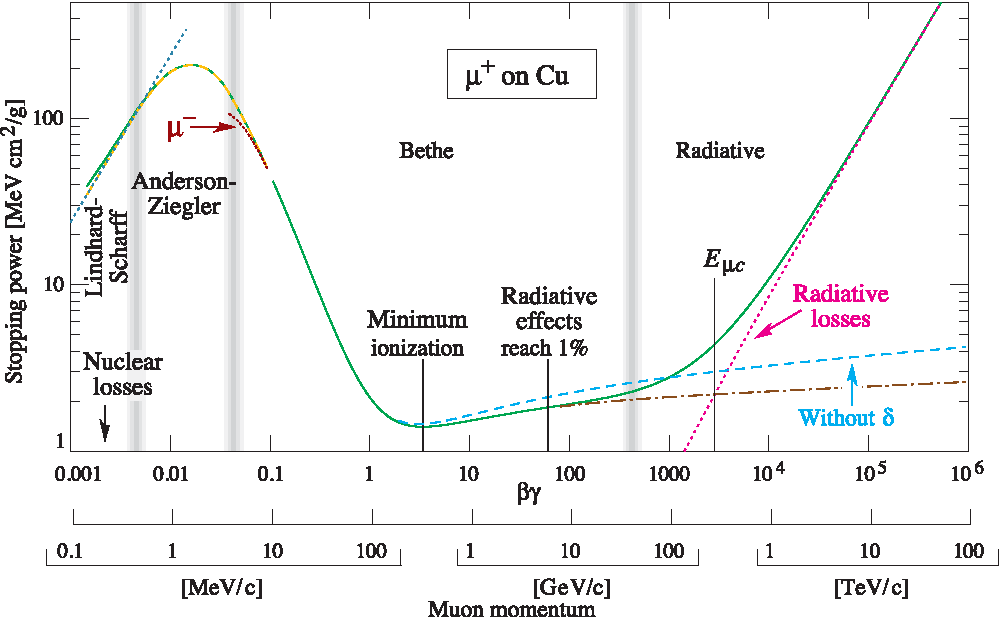
\includegraphics[width=0.95\textwidth]{ECAL/graphics/rpp_icru49_cu.pdf}
	\caption{\label{fig:BB_2} \sl Stopping power or $<-dE/dx>$  for muons in copper as a function of $\beta\gamma = p/mc$, where $m$ is the muon mass, $p$ is muon momentum and $c$ is the speed of light. }
\end{figure}
\subsection{Electromagnetic showers}
The emission of photon or bremsstrahlung process is the dominant process of the energetic electron-matter and positron-matter interaction.
The high-energy photons interact with matter via the convertion to $e^+e^-$ pair.
Thus, passage of these particles in dense materials create an intense cascade of pair creation and photon radiation processes, i.e. electromagnetic cascades or showers.
Eventually, the electron energy falls below the critical energy of the bremsstrahlung, and then they lose their energy by ionization and atomic excitation processes.
Below the $e^+e^-$ pair convertion threshold, the photons lose their energy in the material by the Compton scattering process. 

The main characteristic of the material is the radiation length $X^0$, defined as the mean distance over which a high-energy electron loses all but $1/e$ of its energy, or $7/9$ of the mean free path of a high-energy photon. 
The transverse size of the electromagnetic cascade is described by Moli\`ere radius $R_{m}$, which is defined as an average radius of a cylinder containing 90\% of an electromagnetic cascade. Moli\`ere radius is proportional to the radiation length of the material. 
The radiation length and the Moli\`ere radius values for various materials are shown in Table~\ref{table:material}.
        \begin{table}[H]
        \begin{center}
        \begin{tabular}{l c c c c}
        \hline
	Material & $X_0$ [cm] & $R_m$ [cm] &  $\lambda_{I}$ [cm] & $\lambda_{\pi^{\pm}}$ [cm]  \\
	\hline
	Dry air  & 30390 & 7330 & 74770 & 101300 \\
	Iron Fe  & 1.757 & 1.719 & 16.77 & 20.42 \\
	Lead  Pb & 0.5612 & 1.602 & 17.59 & 19.93 \\
	Tungsten W &0.35&0.93& 9.946 & 11.33 \\ 
        \hline
        \end{tabular}
        \end{center}
        \caption{\sl The material properties of interest for high-energy physics~\cite{bib:PDGprop}. }
        \label{table:material}
        \end{table}


\subsection{Hadronic showers}
All hadrons have an electric and a confined color charge. 
Thus, the charged hadrons can interact with material via ionization process, and all hadrons, neutral and charged ones, can interact with matter nuclei via the strong force.
The strong interaction with matter can be elastic and inelastic. 
The elastic hadron-matter interaction is the nucleus excitation process, via gluon exchange, which do not change the hadron or nuclei composition. 
The inelastic hadron-matter interaction often leads to a spallation of the target nuclei creating new stable or unstable hadrons. 
The emitted relatively energetic  $\pi^0$ and $\eta$ mesons decaying into two photons give a rise to an electromagnetic shower. 
The stable and long-lived hadrons, like pions, protons and neutrons, can escape the collision region. 
Thus, the energy deposit value of the hadronic showers is highly fluctuating. 

The material is characterized by the nuclear interaction length $\lambda_{I}$, which is defined as a mean material length reducing the number of passing by hadrons by the factor of $1/e$. 
Specifically, the pion interaction length $\lambda_{\pi^\pm} > \lambda_{I}$, due to longer mean free path of the $\pi^\pm$ in the same type of material. 
The   $\lambda_{\pi^\pm} $ and $ \lambda_{I}$ values for various materials are given in Table~\ref{table:material}.
\subsection{Simulations}
The most famous toolkit to simulate the passage of particles through matter is \geant\ simulation software~\cite{Allison:2006ve}. 
It is used in a variety of application domains, including high energy physics, astrophysics and space science, medical physics and radiation protection. 
The \geant\ physics processes cover variety of particle-matter interactions over a wide energy range.
The description of highy-fluctuating processes, like hadron-matter interaction, can be done by using different approximations. 
Thus, simulation of the hadron-matter interaction in \geant\ is implemented in physical models called \textit{physics lists}~\cite{bib:G4pl}.

\section{Introduction}
%General introduction

The design of particle detectors at future high-energy physics experiments and, in particular, at linear colliders is oriented towards the usage of Particle Flow algorithms (PFA) for the event reconstruction. 
These algorithms require calorimeters with high granularity to reconstruct individual particles, aiming at the improvement of the jet energy resolution \cite{Brient:2002gh}. 

The primary objective of the CALICE (Calorimeter for the Linear Collider Experiment) collaboration is the development, construction and testing of highly granular hadronic and electromagnetic  calorimeters for future particle physics experiments.

A detailed study of the calorimeter response to particle interactions is necessary to verify existing Monte Carlo simulation models and to build a reliable PFA. 
This implies the precise simulation and reconstruction of the interaction of neutral and charged hadrons and the subsequent particle cascade.

This note reports on a detailed study of hadronic interactions in the CALICE Silicon-Tungsten Electromagnetic Calorimeter (\ecal) physics prototype \cite{Anduze:2008hq}.
The \ecal\ was tested at Fermi National Accelerator Laboratory (FNAL) in 2008 using a beam of $\pi^-$-mesons in the energy range from 2 to 10\,GeV. 
%High energy jets are predominantly composed of neutral and charged pions within this energy range and therefore the performance of Monte Carlo simulations with these particles is important.
The highly granular structure of the \ecal\ permits a detailed measurement of hadronic showers in terms of integral observables \cite{Bilki:2014uep} such as cluster extensions and energy depositions. As will be shown in this note, the high granularity allows in addition for deeper studies of the interactions between the hadrons and the absorber material such as the characterisation of the interaction region and the analysis of secondaries emerging from the interaction. The tracks produced by these secondaries are reconstructed by a new simple \tfa . The resulting observables are subject to comparison of data with predictions from different {\sc Geant}4 Monte Carlo physics lists. The analysis complements studies presented in~\cite{Adloff:2013vra} and~\cite{bib:can-047} for tracking in CALICE prototypes of hadronic calorimeters.  

%and differential observables, like kinematics of secondary particles, that emerge from hadron-detector interactions.


%TODO: insert new results of study if any
%This study is done as an extension of Ref. \cite{bib:Naomi}, where Monte Carlo simulation are compared with data using global observables like lateral and longitudinal extension of the hadronic cascade immediately after the first interaction.
%and they can create energy depositions outside a main hadronic showers. 
%The reconstruction of these secondary tracks provides a new set of observables that can:
%\begin{itemize}
%\item extend Monte-Carlo comparison with experimental data by using kinematic observables of secondary particles;
%\item improve reconstruction of the energy of neutral hadrons by detecting distant energy depositions using track information inside calorimeter;
%\item improve Particle ID algorithms by introducing more detailed shower shape information for identification of hadron interaction in the \ecal.
%\end{itemize}
%||||||||||||||||||||||||ECAL|||||||||||||||||||||||%

\section{The \ecalp}
\label{sec:ecal}
The \ecalp\ has a sandwich-like structure comprising 30 layers of silicon (Si) as active material, alternated with tungsten (W) as absorber material. The active layers are made of Si wafers segmented in 1 $\times$ 1\,cm$^2$ pads. As shown in Fig. \ref{fig:ECAL-scheme}, each wafer consists of a square of 6 $\times$ 6 pads and each layer is a matrix of 3 $\times$ 3 of these wafers resulting in an active zone of 18 $\times$ 18\,cm$^2$.
\begin{figure}[H]
	\centering
	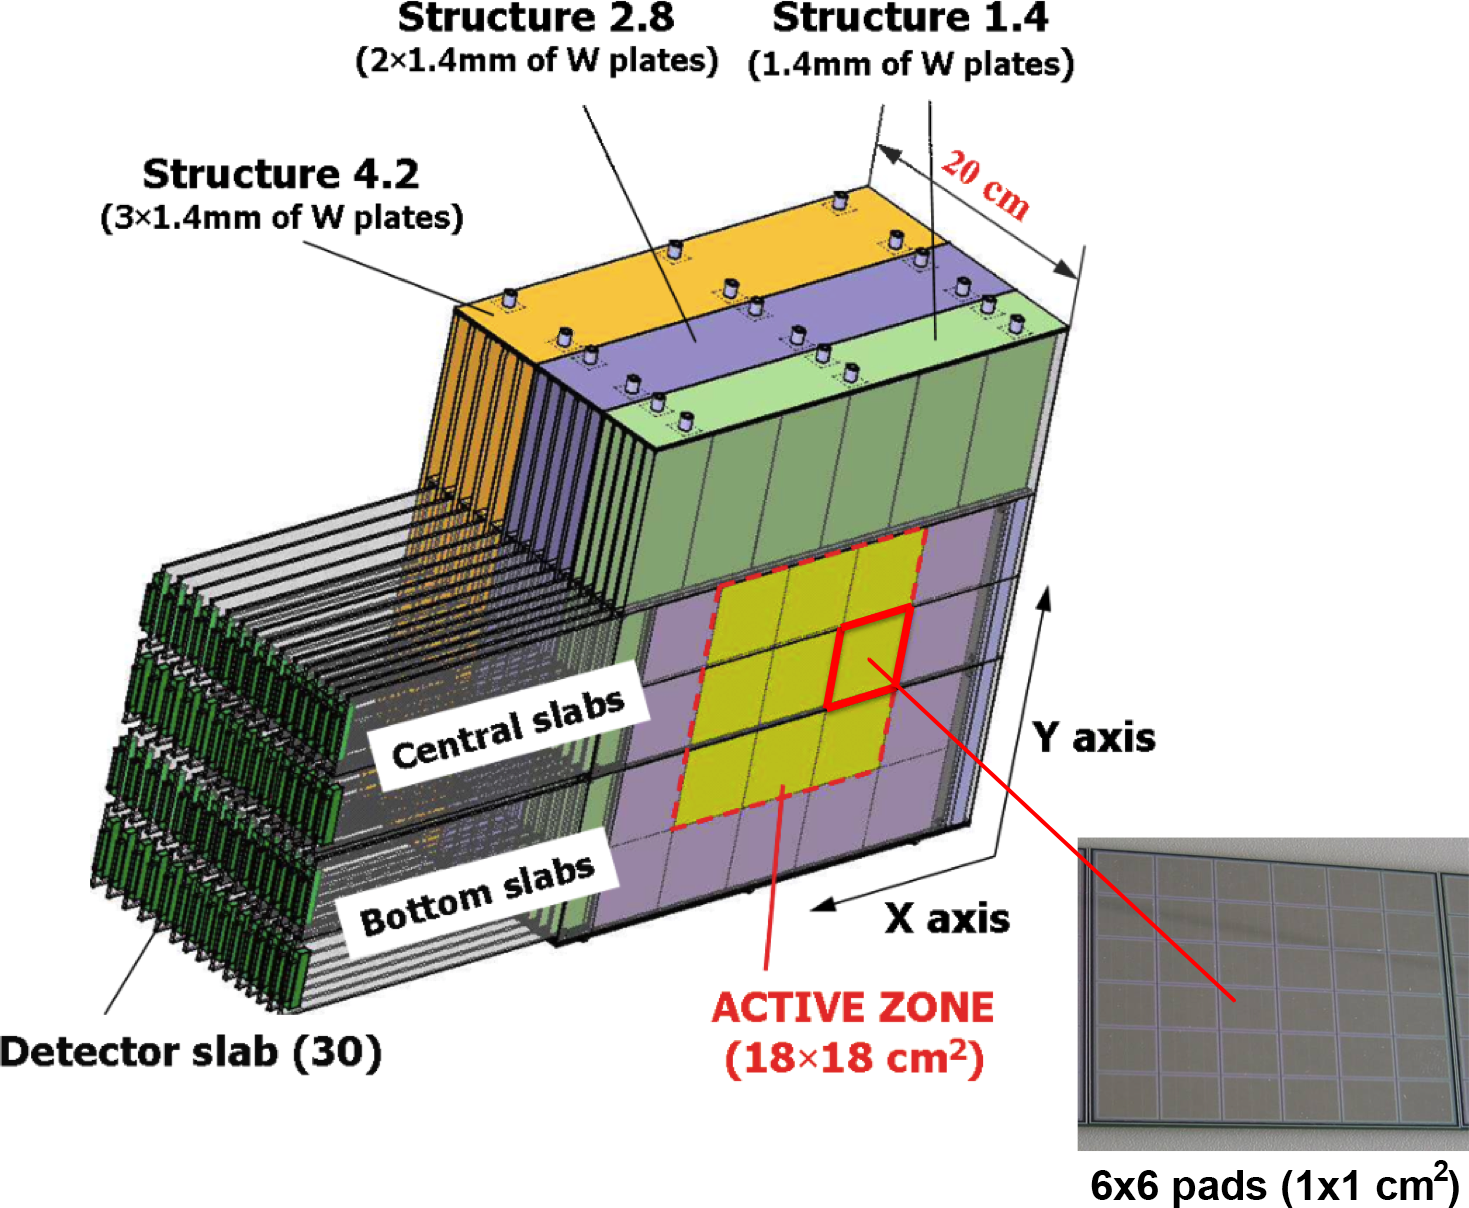
\includegraphics[width=0.5\textwidth]{ECAL/graphics/ecal-new.png}
	\caption{\label{fig:ECAL-scheme} \sl A schematic view of the \ecalp.}
\end{figure}
The \ecal\ is subdivided into 3 modules of 10 layers each. The W depth per layer is different in each module increasing from 1.4\,mm (0.4 radiation lengths or $X_0$) in the first one, to 2.8\,mm in the second and 4.2\,mm in the last one. The total thickness corresponds to 24 $X_0$ or about 1 nuclear interaction length $\lambda_I$ which ensures that more than half of the hadrons will have a primary interaction within the detector volume.
%This frame is used for the clustering and tracking algorithm, described in Sec. \ref{sec:track}.
%The direction of $z$-axis is parallel to the primary particle momentum.
A more detailed description of the prototype can be found in \cite{Anduze:2008hq}.

%|||||||||||||||||||Description of a dataset||||||||||||||||||||%

\section{Data and Monte Carlo samples}
\label{sec:data}
\subsection{Experimental setup at FNAL}\label{sec:fnal}
The test beams were carried out at the Fermilab Test Beam Facility\footnote{\label{note1}Fermilab Test Beam Facility web page: \url{http://www-ppd.fnal.gov/MTBF-w}}, FTBF, at FNAL in May and July 2008.
The \ecal\ was placed in front of two other CALICE physics prototypes: an AHCAL \cite{collaboration:2010hb} and a TailCatcher (TCMT) \cite{CALICE:2012aa}.
The beam-line comprised in addition two scintillator counters, covering an area of 10 $\times$ 10 cm$^2$, for triggering on incoming particles and two Cherenkov detectors for particle identification.
The chosen coordinate system is right-handed with the $z$-axis pointing along the beam direction and the $y$-axis being vertical.
The analysed data in this note comprise runs with primary $\pi^-$-mesons. The energies of the primary particles are 2, 4, 6, 8 and 10 GeV.

\subsection{Monte Carlo simulations}

%Due to the complicated nature of hadronic interactions a precise description of hadronic showers in simulations is difficult to achieve. 
Monte Carlo simulations were carried out within the Mokka framework~\cite{MoradeFreitas:2002kj}, which provides the geometry interface to {\sc Geant}4~\cite{Allison:2006ve}. 
There are several simulation models of hadronic interactions available within {\sc Geant}4, that are combined into so-called \textit{physics lists}.
Each model has its own theoretical basis valid mainly in a specific energy range of hadrons. In this analysis, three physics lists contained in {\sc Geant4} version 10.01 are compared with the experimental data:
\begin{itemize}
	\item \qgsp\ combines the Bertini model
	at energies below 9.9\,GeV, with the Low Energy Parametrised model at energies above 9.9\,GeV;
	\item \ftfp\ has a transition from the Bertini model to the Fritiof model around a primary particle energy of 4.5\,GeV.
	\item \qbbc also intrapolates between the Bertini model and the Fritiof model however with a larger transition region.
\end{itemize}
The physics lists are illustrated in Fig.~\ref{fig:physicslist_2}.
\begin{figure}
	\centering
	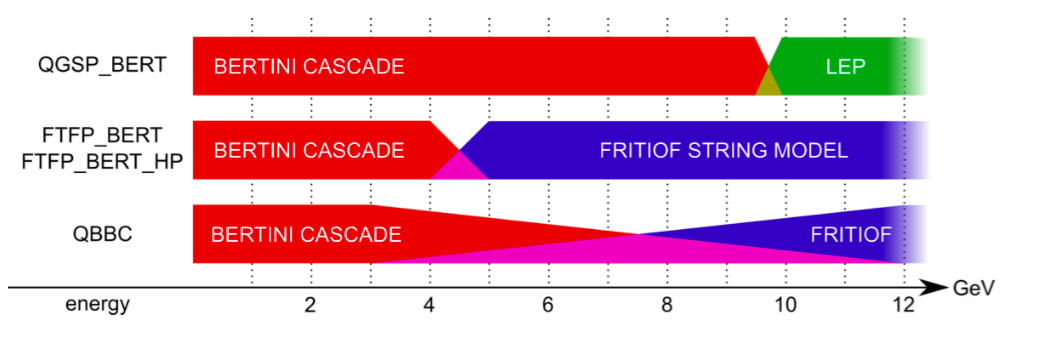
\includegraphics[width=0.95\textwidth]{ECAL/graphics/physics-lists.png}
	\caption{\label{fig:physicslist_2} \sl Illustration of the transitions between the different physics models within the used \geant\ physics lists.  }
\end{figure}
More information about these and other physics lists can be found in \cite{bib:G4pl}.

\subsection{Event selection and preprocessing}

The FNAL $\pi^-$ test beam is contaminated with $\mu^-$ and $e^-$, in particular at lower energies where the beam is dominated by $e^-$. 
At 2 GeV the beam contains about 5\% of $\pi^-$ mesons and 70\% of electrons. 
Events are triggered using the signals from the two scintillator counters upstream of the \ecal\ and $\pi^-$ are identified by using Cherenkov counters.
The response of the \ecal\ to charged particles was calibrated with  an energetic $\mu^-$ beam \cite{li:tel-00430432} and the hit energy is converted into units of most probable energy depositions by minimum ionising particles (MIP). 
%Muons penetrate the whole detector volume with a nearly identical energy loss rate which is minimal for the beam energy used. 
%These $\mu^-$ are so-called minimum ionising particles or MIP and their mean energy loss in the active medium of a pad defines the energy unit MIP.

To select $\pi^-$ showers the data and simulation samples undergo the following selection steps \cite{Bilki:2014uep}\cite{doublet:tel-00657967}: 
\begin{itemize}
	\item A series of cuts is applied to reject multi-particle events caused by beam impurities or products of decays or upstream interactions of primary particles. The influence of residual multi-particle events will be discussed in Sec.~\ref{sec:results};
	\item A threshold of 0.6 MIP is chosen to remove noisy hits in the \ecal;
	\item A hit is removed as being isolated if all the 26 pads in the surrounding cube have no signal above the noise threshold. The analysis presented in this note applies to the non-isolated hits that remain after this removal. The term hits will continue to be used.   
	\item The total number of hits in the ECAL is required to be at least 25 to remove particles with large incident angle;
	\item The barycentres of the transverse coordinates $\bar{x}_{hit}$ and $\bar{y}_{hit}$ of the hits are calculated as:
	\begin{eqnarray}
	\label{eq:barycentre}
	\bar{x}_{hit} = \frac{\displaystyle \sum_{hits} x_{hit}\,E_{hit}}{\displaystyle \sum_{hits} E_{hit}} 
	\text{ and }
	\bar{y}_{hit} = \frac{\displaystyle \sum_{hits} y_{hit}\,E_{hit}}{\displaystyle \sum_{hits} E_{hit}},
	\end{eqnarray}
	where $E_{hit}$ is the energy of a hit in MIP units, and the sums run over all hits in the calorimeter.
	The event is accepted if $-50\,{\rm mm} < \bar{x}_{hit} < 50\,{\rm mm}$ and $-50\,{\rm mm} < \bar{y}_{hit} < 50\,{\rm mm}$ to
	reduce lateral shower leakage;
	\item  In first approach the interaction layer $i$ is identified with the first of three consecutive layers for which
	\begin{equation}
	E_i > E_{cut}, E_{i+1} > E_{cut}  \text{ and } E_{i+2} > E_{cut}.
	\end{equation}
	This simple condition is inefficient at small energies and is complemented by using the following relative energy increase
	\begin{equation}
	\frac{E_i+E_{i+1}}{E_{i-1} + E_{i-2}} > F_{cut} \text{ and } 
	\frac{E_{i+1}+E_{i+2}}{E_{i-1} + E_{i-2}} > F_{cut}, 
	\end{equation}
	with $E_i$ being the total energy of layer $i$. The variables $E_{cut}$ and $F_{cut}$ are free parameters with empirical values of 8 MIP and 6, respectively. It is argued in \cite{Bilki:2014uep} and references therein that these values optimise the selection efficiency in the energy range relevant for the present study.
	The event is selected if $5 < i < 15$ to suppress electron contamination and to assure "long" secondary tracks after the interaction.
	%\item a cut on minimal number of hits in  two last layers of \ecal\ was applied to reduce number of events with elastic scattering.
\end{itemize}
%This selection scheme originally developed and used in \cite{bib:Naomi}\cite{bib:2012_Doublet}.
%Preselect the events, which have an energy deposition at the last layers of the ECal and interaction in the first half of the Ecal

%---------------------------------------------------------------
%----------------------------TFA--------------------------------
%---------------------------------------------------------------

\section{The \tfa}
\label{sec:track}

%\subsection{Algorithm description}
%The outgoing charged secondary particles in hadron interactions leave tracks in the \ecal. 
%These tracks are reconstructed by a  new simple \tfa\. 
%The resulting observables is used for comparison of different {\sc Geant}4 Monte Carlo simulations with experimental data, taken at FNAL in 2008. 
%Identification of tracks in hadronic showers is useful for precise energy calculation in PFA and for more detailed comparison of experimental data and Monte Carlo simulations. 
%The \tfa\ developed here is oriented on a Monte Carlo comparison study for \ecalp\ using new set of observables, based on properties of secondary particles from hadronic interactions. 

The main objective of the \tfa\  is the detection of forward-scattered tracks from the interaction between the primary pions and the absorber material in the absence of a magnetic field.

The designed algorithm has the following execution scheme:
\begin{itemize}
	\item After the selection cuts, see Sec. \ref{sec:data}, the interaction region is identified and singled out. The interaction region will be defined in Sec.~\ref{sec:iazone};
	\item The remaining energy depositions are used for clusterisation;
	\item The obtained clusters are classified to select track-like clusters from residual noise; %and interaction region clusters.
	\item After classification different clusters from a single outgoing secondary particle are merged into one track.
\end{itemize}
The entire algorithm is executed on a unit grid based on the \ecal\ pad identifiers according to 
%pad identifier
\begin{equation}
\vec{x} = (x,y,z)=\left
\{
\begin{array}{c}
x= 0 .. 17 \\ 
y=0 .. 17 \\
z = 0 .. 29,
\end{array}
\right.
\end{equation}
where pad counting starts in the bottom right pad, see Fig.~\ref{fig:ECAL-scheme}. Distances in this grid are measured in {\em grid units}, ${\rm g.u.}$  



%|||||||||||||||||||Interaction zone|||||||||||||||||||||||

\subsection{Removing the interaction region}
\label{sec:iazone}
A typical inelastic hadronic interaction in the \ecal\ creates a shower with an interaction region and tracks of long-lived particles emerging from it. The interaction region is created by particles with a short distance of flight in the absorber material of the \ecal, like electrons, photons and low momentum hadrons. 

In the present analysis the interaction region is defined by all hits that have at least six neighbouring pads with a signal above the noise threshold. In this sense the neighbouring pads are always also part of the interaction region, which applies in particular at the border of the interaction region. The minimal value of six pads is chosen such that muon events remain unaffected meaning that a fake interaction region is found in only 1\% of single muon events. On the other hand for a value of five neighbouring pads about 10\% of muon events would get assigned a fake interaction region. Increasing the minimal value to seven neighbouring pads with hits reduces the fraction of events with a fake interaction still a bit but does not alter the results presented in the following.

%The interaction region removal follows a principle similar to that of the isolated hit filter: a hit belongs to the interaction region if it has a number of neighbor hits above a certain threshold. The threshold value of 6 pads is chosen to leave  $\mathrm{\mu}^-$ events unaffected.
\begin{figure}
	\centering
	\begin{subfigure}{0.5\textwidth}
		\centering
		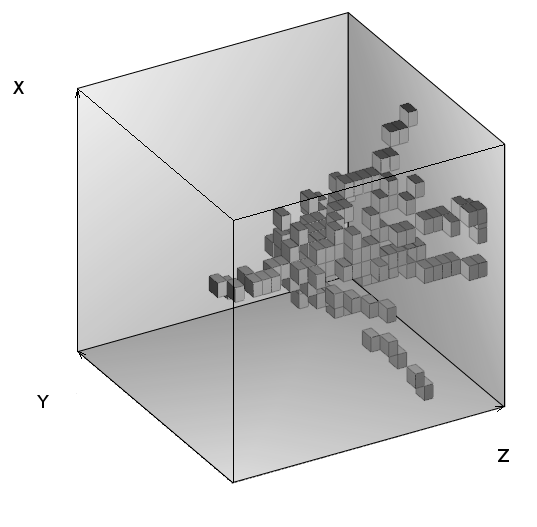
\includegraphics[width=.90\linewidth]{ECAL/graphics/before.png}
		\caption{\label{fig:before} \sl with interaction region.}
	\end{subfigure}% 
	\begin{subfigure}{0.5\textwidth}
		\centering
		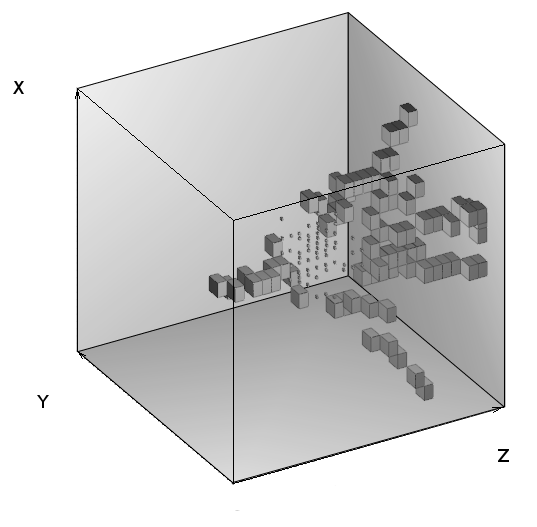
\includegraphics[width=.90\linewidth]{ECAL/graphics/after2.png}
		\caption{\label{fig:after} \sl without interaction region.}
	\end{subfigure}
	\caption{ \sl {\bf Propose to show a real event} Event display of a primary pion with an energy of 10\,GeV simulated using the \ftfp\ physics list before \textit{(a)} and after removal of the interaction region \textit{(b)}. Smaller cubes are pads that are part of the interaction region and are not processed by the \tfa . In this event the hits in the first ten layers are classified as hits left by a primary particle.}
	
	\label{fig:test}
\end{figure}

Figure \ref{fig:before} displays a simulated event after noise and isolated hits filters and Fig. \ref{fig:after} is the same event after removal of the interaction region. As can be seen in Fig. \ref{fig:after} the interaction region is the starting point for secondary tracks.

%The energy deposition in the interaction region of the $\mathrm{\pi}^-$ events in \ecal\ is analyzed in Sec. \ref{sec:results}.

%|||||||||||||||||||||||clusterisation||||||||||||||||||||||||||||

\subsection{Clusterisation}\label{sec:cluster}
During the clusterisation step the energy depositions that are not associated to the interaction region are grouped into clusters by a topological principle. %This step is needed to separate secondary tracks into corresponding groups of hits, or clusters, for further classification. 

\begin{figure}
	\centering
	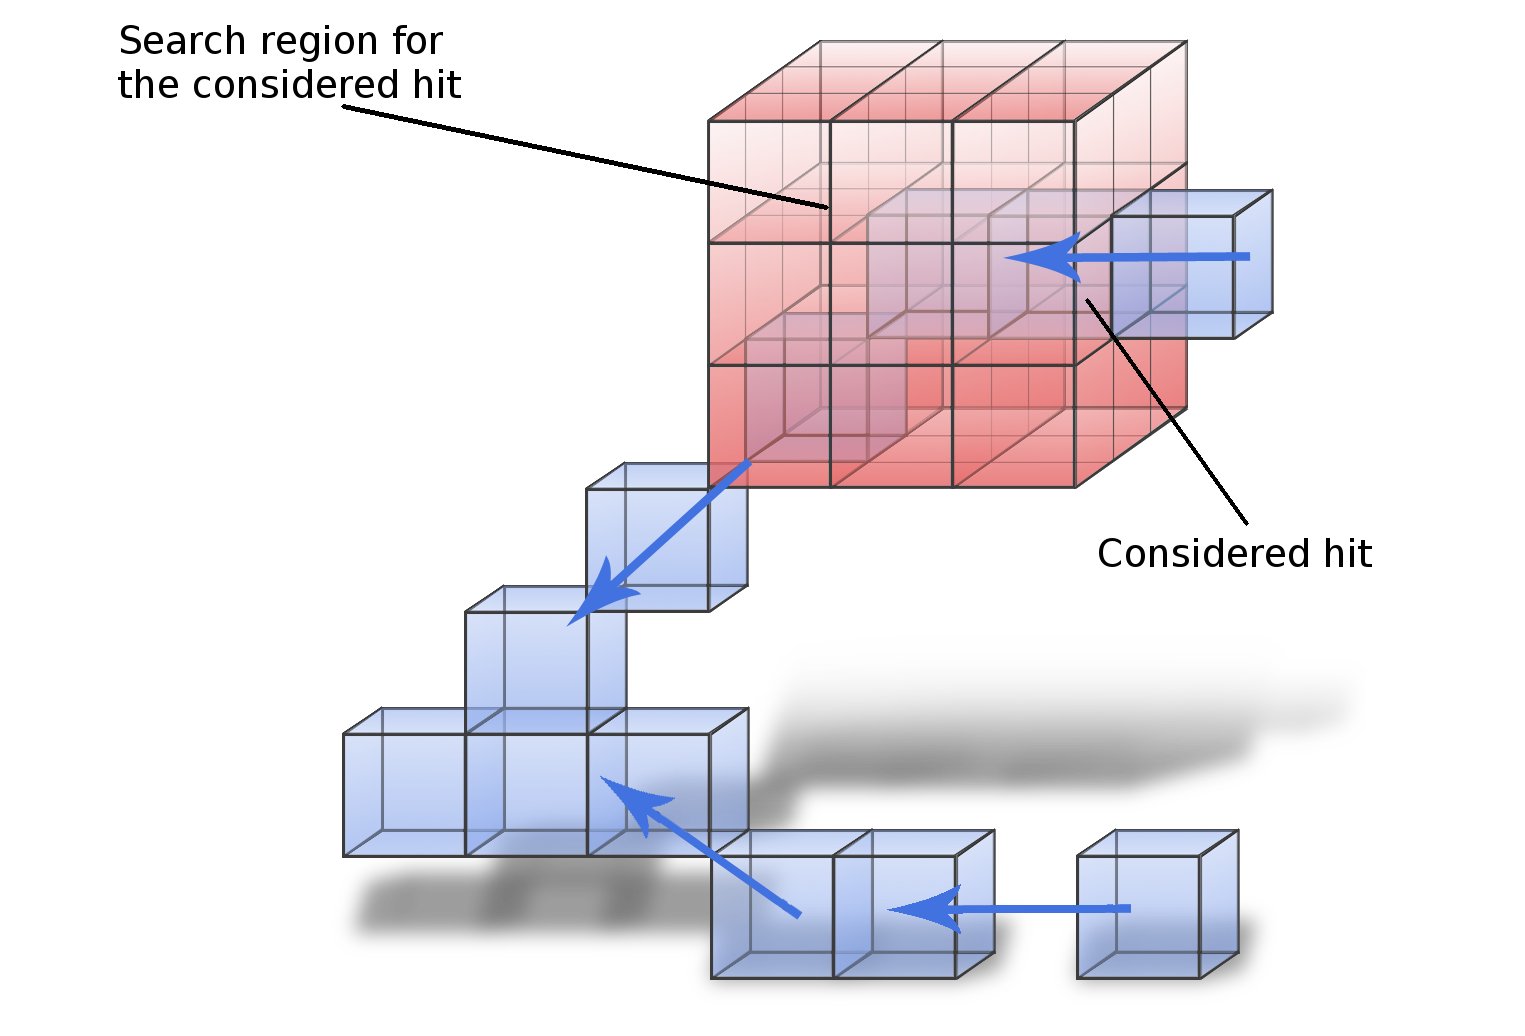
\includegraphics[width=0.5\textwidth]{ECAL/graphics/demo-v2.png}
	\caption{\label{fig:democluster} \sl {\bf Check comment by Eigen on clarity of image} Illustration of the clusterisation step. The \ecal\ hits are represented by blue cubes, and the search region for adjacent hits is indicated by red cubes. The blue arrows point in the direction of the clusterisation flow. }
\end{figure}

%A clusterisation scheme, developed for this study, is called directional recursive clusterisation. 
%The clusterisation algorithm starts recursive assembling of clusters from the last layers of the \ecal, where the secondary tracks are more distinguishable, until the interaction zone or until the first layers in case of MIP-like events. 

The algorithm is described in the following. The description is supported by Fig.\ \ref{fig:democluster}.
%his algorithm has the following steps:
\begin{enumerate}
	\item The separation of tracks improves with increasing distance from the interaction layer. Therefore, hits, isolated within one of the rear layers, seed a cluster. The search for these hits is carried out progressively starting from the last layer in the direction of decreasing $z$.
	Typically, seeding hits are found in the last layer of the detector;
	%For each iteration, the seeding hits for the clusters are taken starting from the last layers of pads to the front layer;
	\item A hit can be associated to a cluster if it was not yet joined to another cluster. This condition excludes the double counting of hits. Effects, arising from ambiguities in the assignment of hits to clusters such as the order in which clusters are created, are expected to be small, but will be addressed in future studies {\bf We haven't addressed this yet!};
	\item For the clusterisation a usual nearest neighbour clustering scheme is applied. More precisely, for each newly associated hit with coordinates $(x_n,y_n,z_n)$ the algorithm finds nearby hits with the following conditions:
	\begin{itemize}
		\item A neighbour hit should have a $z$ coordinate within $[z_n-2,z_n]$
		\item The transverse coordinates of neighbouring hits is searched within ranges $[x_n-1,x_n+1]$ and $[y_n-1,y_n+1]$
	\end{itemize}
	The search region for nearby hits is visualised  in Fig.~\ref{fig:democluster} as a "red cube" with 3 $\times$ 3 $\times$ 3 pads; 
	%with $z$ coordinate equal or less than $z$ coordinate of considered hit
	\item  For each newly associated hit the Steps 2 and 3 are repeated until the process reaches the first layer of the calorimeter or until no more neighbour hits are found.
\end{enumerate}
The choice of this clusterisation method is motivated by a maximum correspondence between the number of clusters and the number of detected tracks.

%|||||||||||||||||||||||Classification||||||||||||||||||||||||||

\subsection{Classification and merging}
\label{sec:class}
Long-lived charged secondary particles from hadronic interactions are expected to leave straight MIP-like tracks in the detector.
The goal of the classification of the clusters obtained in the previous step is thus to select track-like clusters. %and reject clusters left by electromagnetic interaction or detector noise.
%A track-like cluster is defined as a cluster with hits, spatially arranged in the way, that a trajectory of a single charged particle can go through the most of its pads with energy depositions.

The classification algorithm executes the following steps:
\begin{enumerate}
	\item Reject all clusters with 2 hits ($N_{hits}$) as residual noise clusters;
	\item Calculate the length $l$ of the considered cluster as the maximal distance between any pair of hits that are in the cluster;
	\item A cluster is rejected if it has a length of less than $l_{cut} = 2\,{\rm g. u.}$, which corresponds to the minimal length of a track-like cluster with 3 hits; 
	\item Compute  the following observable:
	\begin{equation}
	\label{eq:observable}
	\xi = \frac{l}{N_{hits}-1} + \varepsilon N_{hits},
	\end{equation}
	as a measure for the eccentricity of the cluster. 
	The first term of Eq.~\ref{eq:observable} in motivated by the linear dependence of $N_{hits}-1$ on the cluster length $l$, illustrated in Fig.~\ref{fig:lnhits}.
	The second term introduces a free parameter $\varepsilon$ as an ad hoc correction to increase the efficiency for selecting clusters that do not conform to the nominal pencil-like topology, as explained below.
	The value of the parameter was chosen to be $0.03$ after visual inspection of a few tens of events in the event display;
	%In Eq. \ref{eq:observable} $\varepsilon$ is a free parameter to correct for non-ideal pencil like clusters. 
	%The parameter $\varepsilon$ takes values much smaller than 1. 
	\item If $\xi \geq 1$ a cluster is considered as track-like. Otherwise, the cluster can be classified as e.g. two inseparable tracks.
\end{enumerate}
Due to a number of effects like multiple scattering, residual detector-noise, $\delta$-rays or the residual arbitrariness in the assignment of hits to clusters, the reconstructed tracks are in general not exactly pencil-like.  
The correction term $\varepsilon N_{hits}$ in the definition of $\xi$ serves to keep a cluster as track-like even if it has large $N_{hits}$ and its form is not strictly pencil-shaped, i.e. $l / (N_{hits}-1) < 1$.

A deeper discussion of the effects of the  \ep\ is presented in Sec. \ref{sec:systematics}. 

\begin{figure}
	\centering
	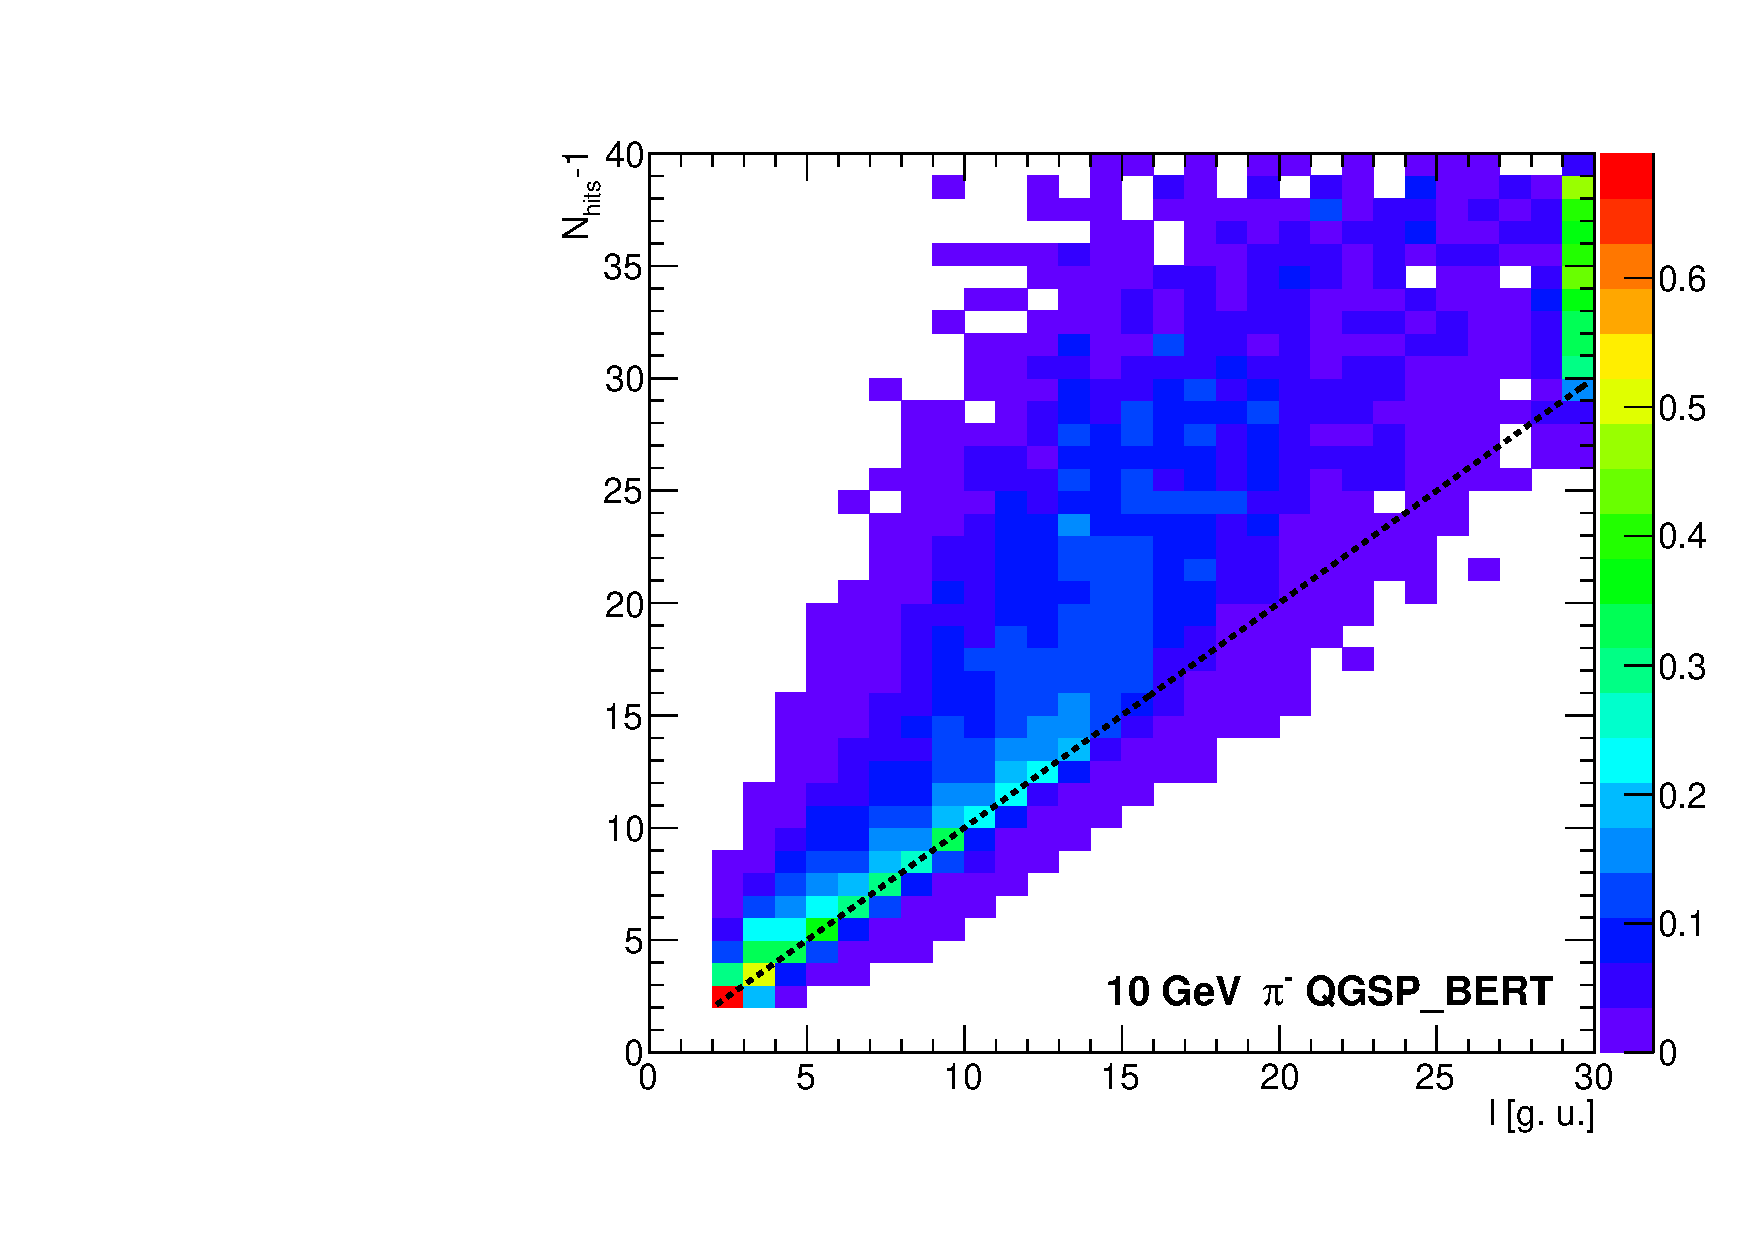
\includegraphics[width=0.5\textwidth]{ECAL/plots/l-nhits.pdf}
	\caption{\label{fig:lnhits} \sl Correlation between $N_{hits} - 1$ and cluster length $l$ in ${\sl g.u.}$ at the example of simulated pions with an energy of 10\,GeV using the \qgsp\ physics list. To guide the eye a line for $N_{hits} - 1=l$ is included in the figure.}
\end{figure}


\begin{figure}
	\centering
	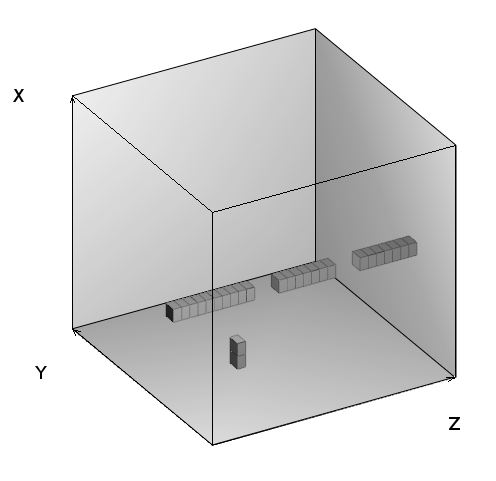
\includegraphics[width=0.5\textwidth]{ECAL/graphics/segmented-track-example.png}
	\caption{\label{fig:demomerge} \sl An example of a segmented track in the \ecal\ from a single 6\,GeV $\mu^-$ in \ftfp\ Monte Carlo simulation.}
\end{figure}
The next step of the classification is to detect a cluster from the primary particle. 
If this cluster exists and meets the conditions for a track-like cluster, it affects the track counting and merging algorithm.
A cluster is classified as being produced by the primary particle if it starts in the first module of the \ecal\ and if it encloses a small angle with respect to the $z$-axis. 
An example of a cluster by a primary particle is visible in Fig. \ref{fig:after}. Clusters assigned to primary particles are discarded in the following analysis. 

Different track-like clusters that correspond to track segments from a single particle, see Fig. \ref{fig:demomerge}, have to be merged into a single track. 
The merging procedure combines track-like clusters with any type of clusters using a simple cone algorithm.
%Because of limitations of clusterisation method, 
%A segmented track from a secondary particle can be divided into two different clusters as it is shown in Fig. \ref{fig:demomerge}.
%It is thus necessary to merge different track segments from a single particle into one track-like cluster. 
%The merging procedure combines track-like clusters with any type of clusters using a simple cone algorithm. 
%TODO: extend merging?
Tested on a sample of single, isolated muons with an energy of 6\,GeV simulated with the \ftfp\ physics list, the \tfa\ finds correctly only one track with 99.7\% efficiency. The sample contains about 3\% events with segmented tracks. 


%------------------------------------------------------------
%----------------------SYSTEMATICS---------------------------
%------------------------------------------------------------

%\subsection{Study of systematics}
\subsection{Discussion of the \ep }
\label{sec:systematics}


The \tfa\ depends on a number of parameters. The biggest sensitivity of the \tfa\ is expected to be introduced by the empirically defined \ep, see Eq.~\ref{eq:observable}. 
Therefore its influence on the results and a further motivation of the choice of the working point in terms of the \ep\, is given in the following. 

After the cut on the minimum cluster length $l_{cut}$, see Sec. \ref{sec:class}, all clusters with 3 hits are track-like, independently of the $\varepsilon$ value.
Therefore, these clusters are not considered in this discussion. 

Figure \ref{fig:epsilonsys} shows the dependence of $\left<N_{tracks}\right>$ on $\varepsilon$ for different beam energies\footnote{\label{note3}The mean number of tracks as function of $\varepsilon$ in data and simulation is given in Appendix~\ref{app:a} for future reference.}.
Each curve has its minimum value at $\varepsilon = 0$ that is the mean number of ideal pencil-like tracks per event and saturates at large $\varepsilon$, when each cluster is taken as track-like.  
%As can be seen from Fig. \ref{sec:systematics} mean number of tracks strongly depend on chosen \ep\ value that needs to be constrained. 
\begin{figure}
	\centering
	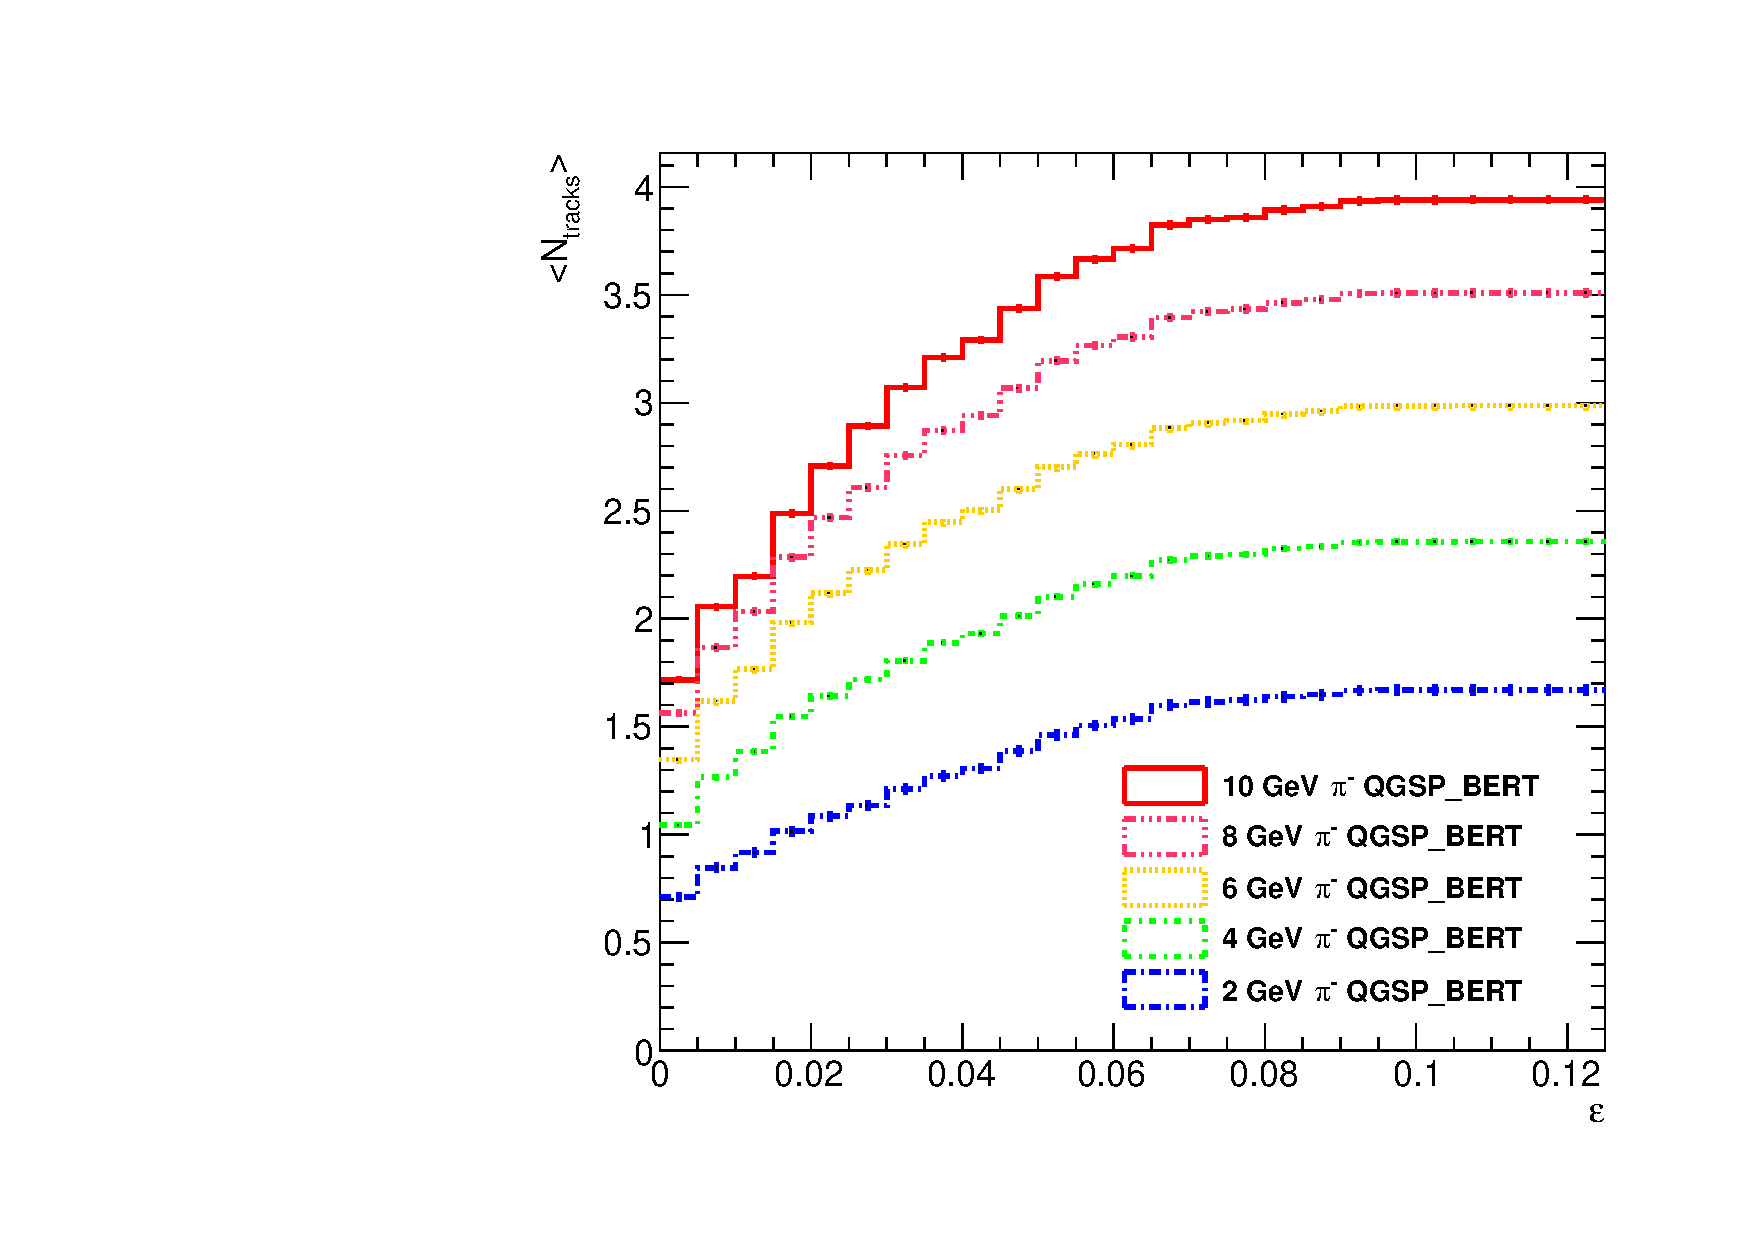
\includegraphics[width=0.5\textwidth]{ECAL/plots/comparison.pdf}
	\caption{\label{fig:epsilonsys} \sl Mean number of tracks found by the \tfa\ as a function of $\varepsilon$ for 2, 4, 6, 8 and 10\,GeV beam energy for the \qgsp\ physics list simulation. Events without a detected interaction region are discarded.}
\end{figure}

For all clusters with a number of hits larger than 3, the simulated muon and electron samples are used to define a motivated choice for the value of  $\varepsilon$ to be applied for the track finding. 

A Monte Carlo sample of $\mu^-$ is used to determine a lower bound on the \ep. The events for this study are selected if the number of hits is larger than the number of layers in the \ecalp. After this cut the muon tracks do not have a straight pencil-like shape, but rather a line with a number of adjacent hits generated by residual detector noise or $\delta$-rays. An example of such a track is given in Fig. \ref{fig:muonsys}.
\begin{figure}
	\centering
	\begin{subfigure}{0.5\textwidth}
		\centering
		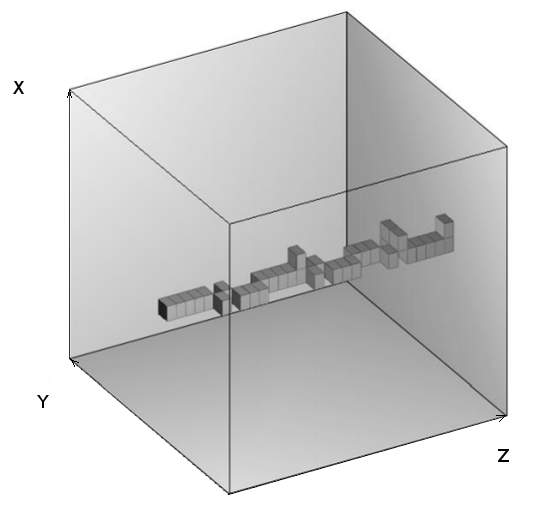
\includegraphics[width=.90\linewidth]{ECAL/graphics/muon-sys.png}
		\caption{\label{fig:muonsys}}
	\end{subfigure}% 
	\begin{subfigure}{0.5\textwidth}
		\centering
		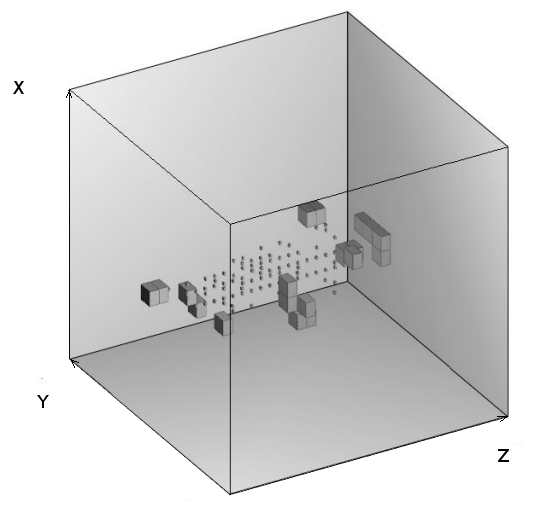
\includegraphics[width=.90\linewidth]{ECAL/graphics/e-sys.png}
		\caption{\label{fig:esys}}
	\end{subfigure}
	\caption{ \sl Event displays of simulated events showing a muon with an energy of 10 GeV after selection by the number of hits in \ecal\ \textit{(a)} and a 6\,GeV electron after removal of the interaction region \textit{(b)}.}
\end{figure}
The resulting sample represents secondary tracks from hadronic interactions with noise or other additional hits from the debris of the interaction region. 

%The electron Monte Carlo sample after the interaction region filter is used to establish an upper bound on the \ep\ value. 
A Monte Carlo sample based on electrons is used to estimate an upper bound on $\varepsilon$. Electrons are not expected to generate tracks but rather only an interaction region accompanied  by low energetic satellite clusters, see Fig~\ref{fig:esys}. Events in this sample contain only non track-like clusters. 
\begin{figure}[H]
	\centering
	\begin{subfigure}{0.5\textwidth}
		\centering
		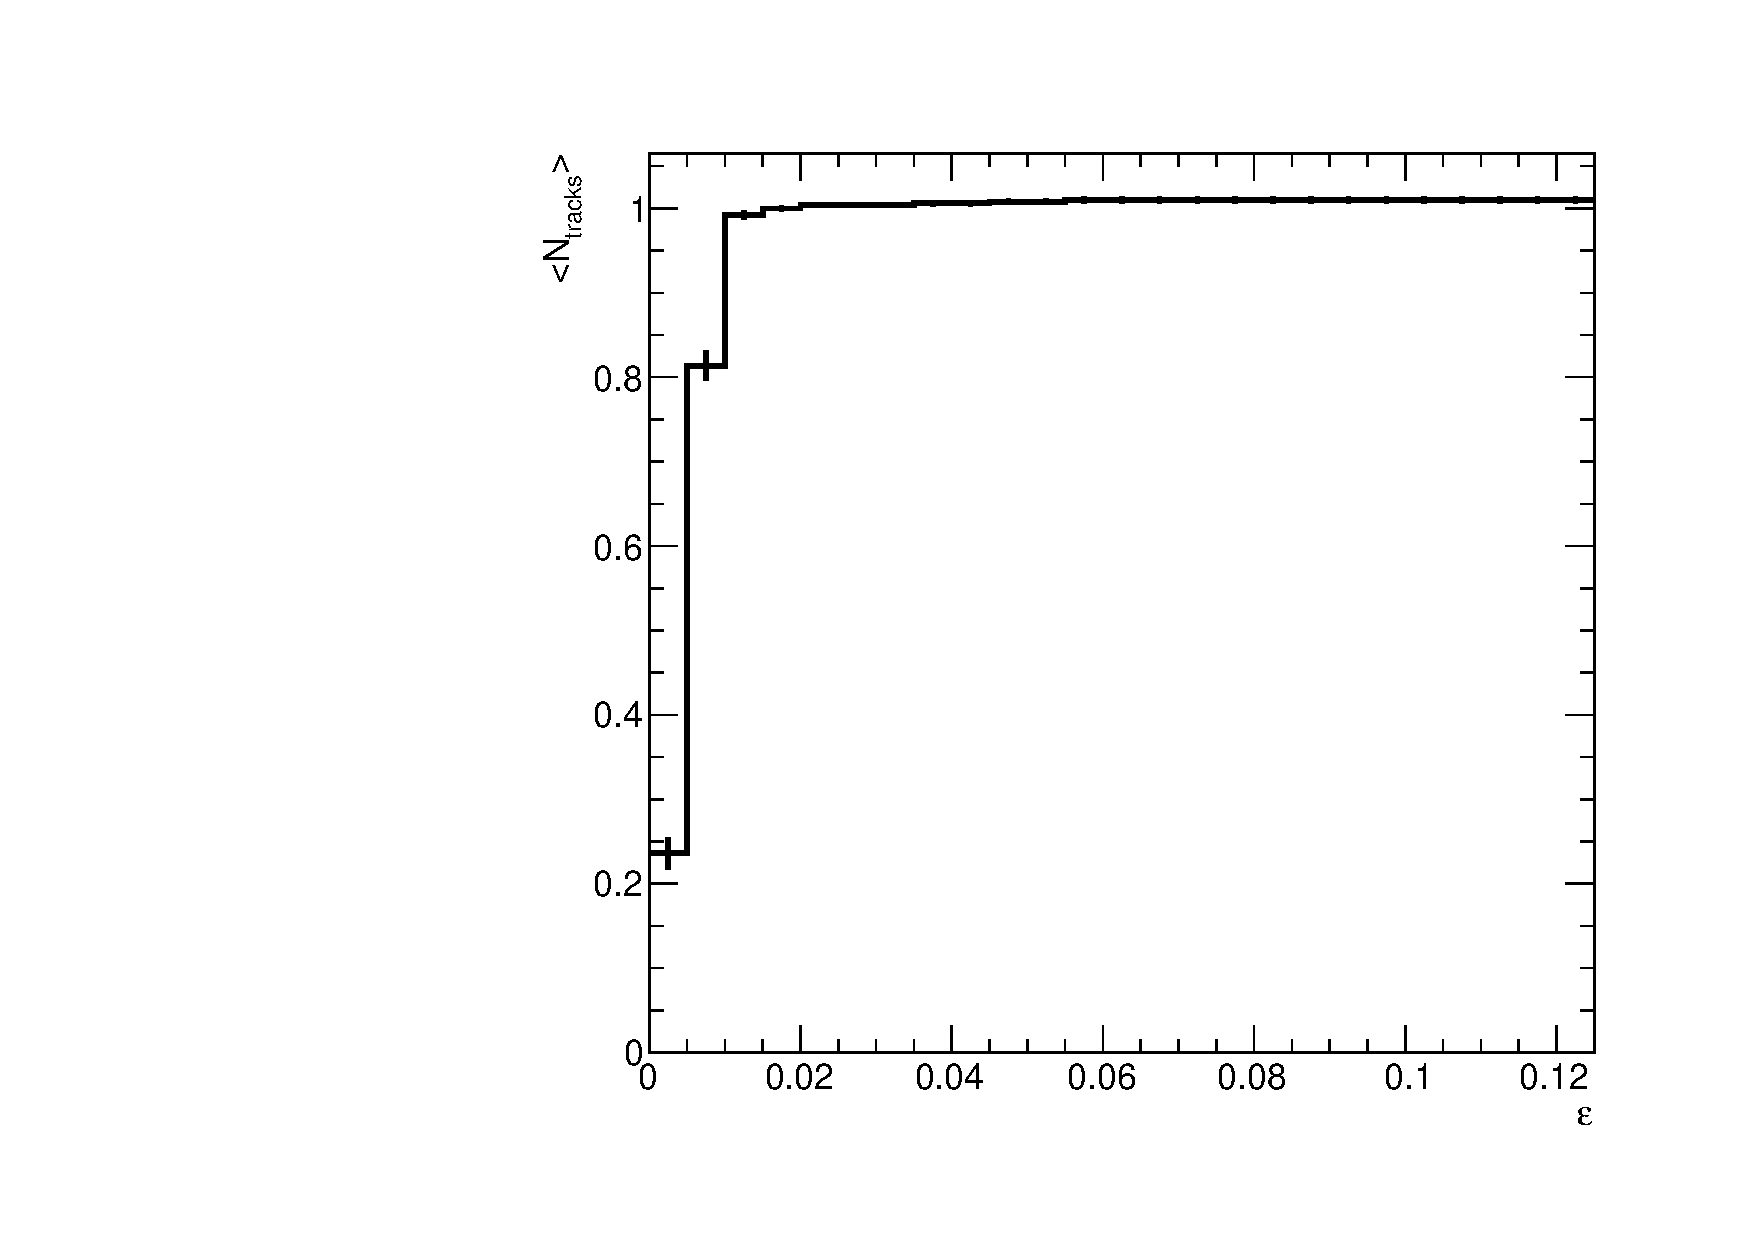
\includegraphics[width=.90\linewidth]{ECAL/plots/muon-sys.pdf}
		\caption{\label{fig:muonhistsys} \sl muon sample}
	\end{subfigure}% 
	\begin{subfigure}{0.5\textwidth}
		\centering
		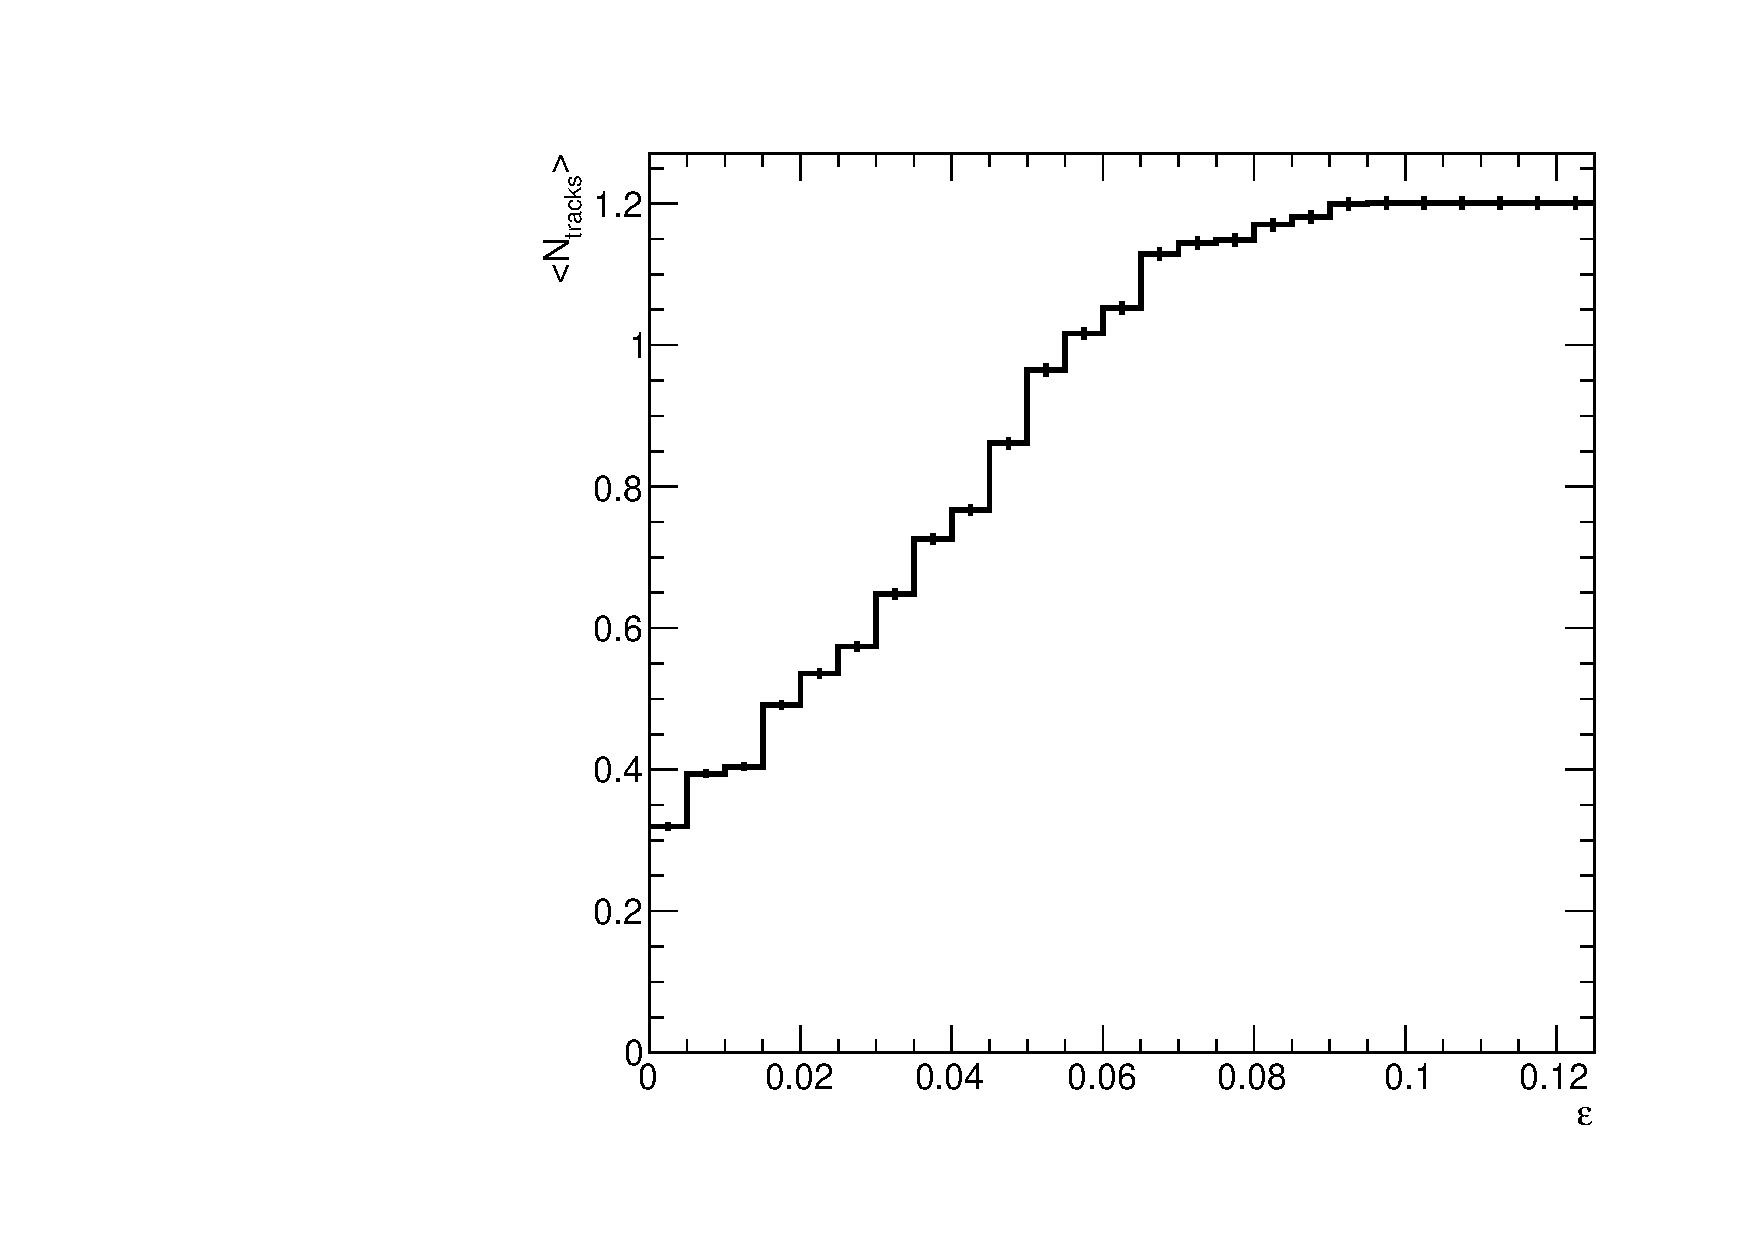
\includegraphics[width=.90\linewidth]{ECAL/plots/electron-sys.pdf}
		\caption{\label{fig:ehistsys} \sl electron sample}
	\end{subfigure}
	\caption{\label{fig:muehistsys} \sl The distribution of $\left<N_{tracks}\right>$ in simulated events as a function of $\varepsilon$ for  \textit{(a)} 10\,GeV $\mathrm{\mu}^-$ after selection by the number of hits in \ecal\ and \textit{(b)} 6\,GeV electrons after removal of the interaction region .}
\end{figure}

Figure \ref{fig:muehistsys} shows the dependence of $\left<N_{track}\right>$ on $\varepsilon$ for the muon (Fig. \ref{fig:muonhistsys}) and electron (Fig. \ref{fig:ehistsys}) samples. 
%The lower bound $\varepsilon_{low}$ on \ep\ value is set to give $N_{tracks} = 1$ on average in muon sample, and upper bound $\varepsilon_{up}$ is defined as $N_{tracks} = 1$ on average in electron sample.
The lower bound $\varepsilon_{low}$ of the \ep\ is identified with the value of $\varepsilon$ for which $\left<N_{tracks}\right> \simeq 1$ in the muon sample. Correspondingly, the upper bound $\varepsilon_{up}$ is identified with that value of $\varepsilon$ for which $\left<N_{tracks}\right> = 1$ in the electron sample.
The approximate values are:
\begin{equation}
\varepsilon_{low} \simeq 0.015\ \texttt{and}\ \varepsilon_{up} \simeq 0.05.
\end{equation}
The empirically chosen value for $\varepsilon$ of $\varepsilon = 0.03$ lies within these bounds. 

As the algorithm is a new development it will be convenient to give the reader a feeling on the sensitivity of the results with respect to the actual choice of the \ep\,
For this the estimator 
\begin{equation}
S_{{\cal O}} = \frac {\left<{\cal O}(\varepsilon_{1}) - {\cal O}(\varepsilon_{2})\right>}  {\left<{\cal O}(\varepsilon_{nom})\right>}
\label{eq:sens}
\end{equation}
is introduced and will be evaluated in Sec.~\ref{sec:results} where applicable.

Further dependencies of the \tfa\ on the value of the cone angle of the merging algorithm, initial MIP exclusion and residual noise are expected to be small but will be addressed for the final paper.
%Other systematic effects coming from value of the cone angle of the  merging algorithm and initial MIP exclusion are expected to be small. %(TODO)

%------------------------------------------------------------------
%---------------------------RESULTS--------------------------------
%------------------------------------------------------------------

\section{Results}
%Systematic uncertainties related to the calorimeter calibration, event selection and preprocessing are discussed in Ref. \cite{bib:Naomi}.
\label{sec:results}
%\subsection{Comparing Monte Carlo models with data}
%Various Monte Carlo models are compared with the test beam data in terms of the interaction region parameters, and secondary tracks observables. The following figures show these comparisons for simulations based on the two studied Monte Carlo physics lists.
In the following observables on the interaction region and on secondary particles as obtained in beam test data are compared with simulations based on the three {\sc Geant4} physics lists introduced above. According to~\cite{Bilki:2014uep} the data are contaminated after the pre-selection with 8.8\% double-$\pi$ events at 2\,GeV and as low as 1.5\% at 10\,GeV. The Monte Carlo samples have thus been produced with an admixture of double-$\pi$ events for the comparison with the data. When averaged results are shown, correction factors will be extracted by comparing the results for contaminated samples with those from pure samples.  The correction factors will be given by the means calculated from the individual correction factors extracted from the two physics lists. The uncertainty on the correction factors will constitute the systematic error and is given by the difference between the mean corrections factor and the individual correction factors. The correction factors are between 0.93 and 1 and the uncertainties are of the order of a few \%. Another source of systematic uncertainty suggested in~\cite{Adloff:2013vra} that may be caused by the uncertainty on the MIP energy scale has been studied and was found to be negligible for the results presented in the following.
%Systematic uncertainties related to the calibration, event selection and preprocessing are discussed in Ref. \cite{bib:Naomi}. 
\subsection{Energy fraction of the interaction region}
%---------------interaction zone--------------------
An intuitive estimator to characterise the interaction of the $\pi^-$  with the absorber material is the fraction $f_{IR}$ of energy deposited in the interaction region $E_{IR}$ over the total energy deposited in the calorimeter $E_{tot.}$. Hence, $f_{IR}$  is defined as
\begin{equation}
f_{IR} = \frac{E_{IR}}{E_{tot.}}
\end{equation}

%In this study the interaction region created by $\pi^-$ interacting with the absorber material is characterised by the fraction $f_{IR}$ of total energy deposited in the calorimeter.% and its lateral radius $r_{IR}$ averaged over hits.

Figure \ref{fig:irexample} shows comparisons of $f_{IR}$ distributions between data and the three {\sc Geant4} physics lists.
The first bin of these histograms corresponds to the fraction of events for which no interaction region is found by the algorithm.
%As can be seen from Fig. \ref{fig:irexample} the fraction of events in this bin for the chosen physics list is approximately(?) compatible with data. 
The rest of the distribution can be briefly described by a skewed normal distribution. The mean value of $f_{IR}$ is shifted towards larger values in data compared with the Monte Carlo simulation. Qualitatively, this observation may suggest for example a different repartition between visible and invisible energy in data and Monte Carlo.

In Fig. \ref{fig:irgraph} the mean value of $f_{IR}$ is shown as a function of the beam energy  for beam energies of 2, 4, 6, 8 and 10\,GeV. Events without a detected interaction region according to Sec.~\ref{sec:iazone} are discarded. An increase of $f_{IR}$ with increasing beam energy from 43\% at 2\,GeV to around 64\% around is observed. Qualitatively this is expected as the electromagnetic component of the hadronic shower becomes increasingly dominant with increasing energy of the primary particle.
In case of the \qgsp\ and \qbbc\  physics list the mean value is up to 20\% smaller than observed in the data.  The \ftfp\ physics list changes its behaviour above 4\,GeV, i.e. at the sharp transition between the Bertini cascade and the Fritiof model bringing the prediction closer to the data.  
The observed discrepancy between data and the predictions by the {\sc Geant4} physics lists is consistent with an underestimation of the total energy deposition by the Monte Carlo models as reported in~\cite{Bilki:2014uep}.


\begin{figure}
	\centering
	\begin{subfigure}{0.5\textwidth}
		\centering
		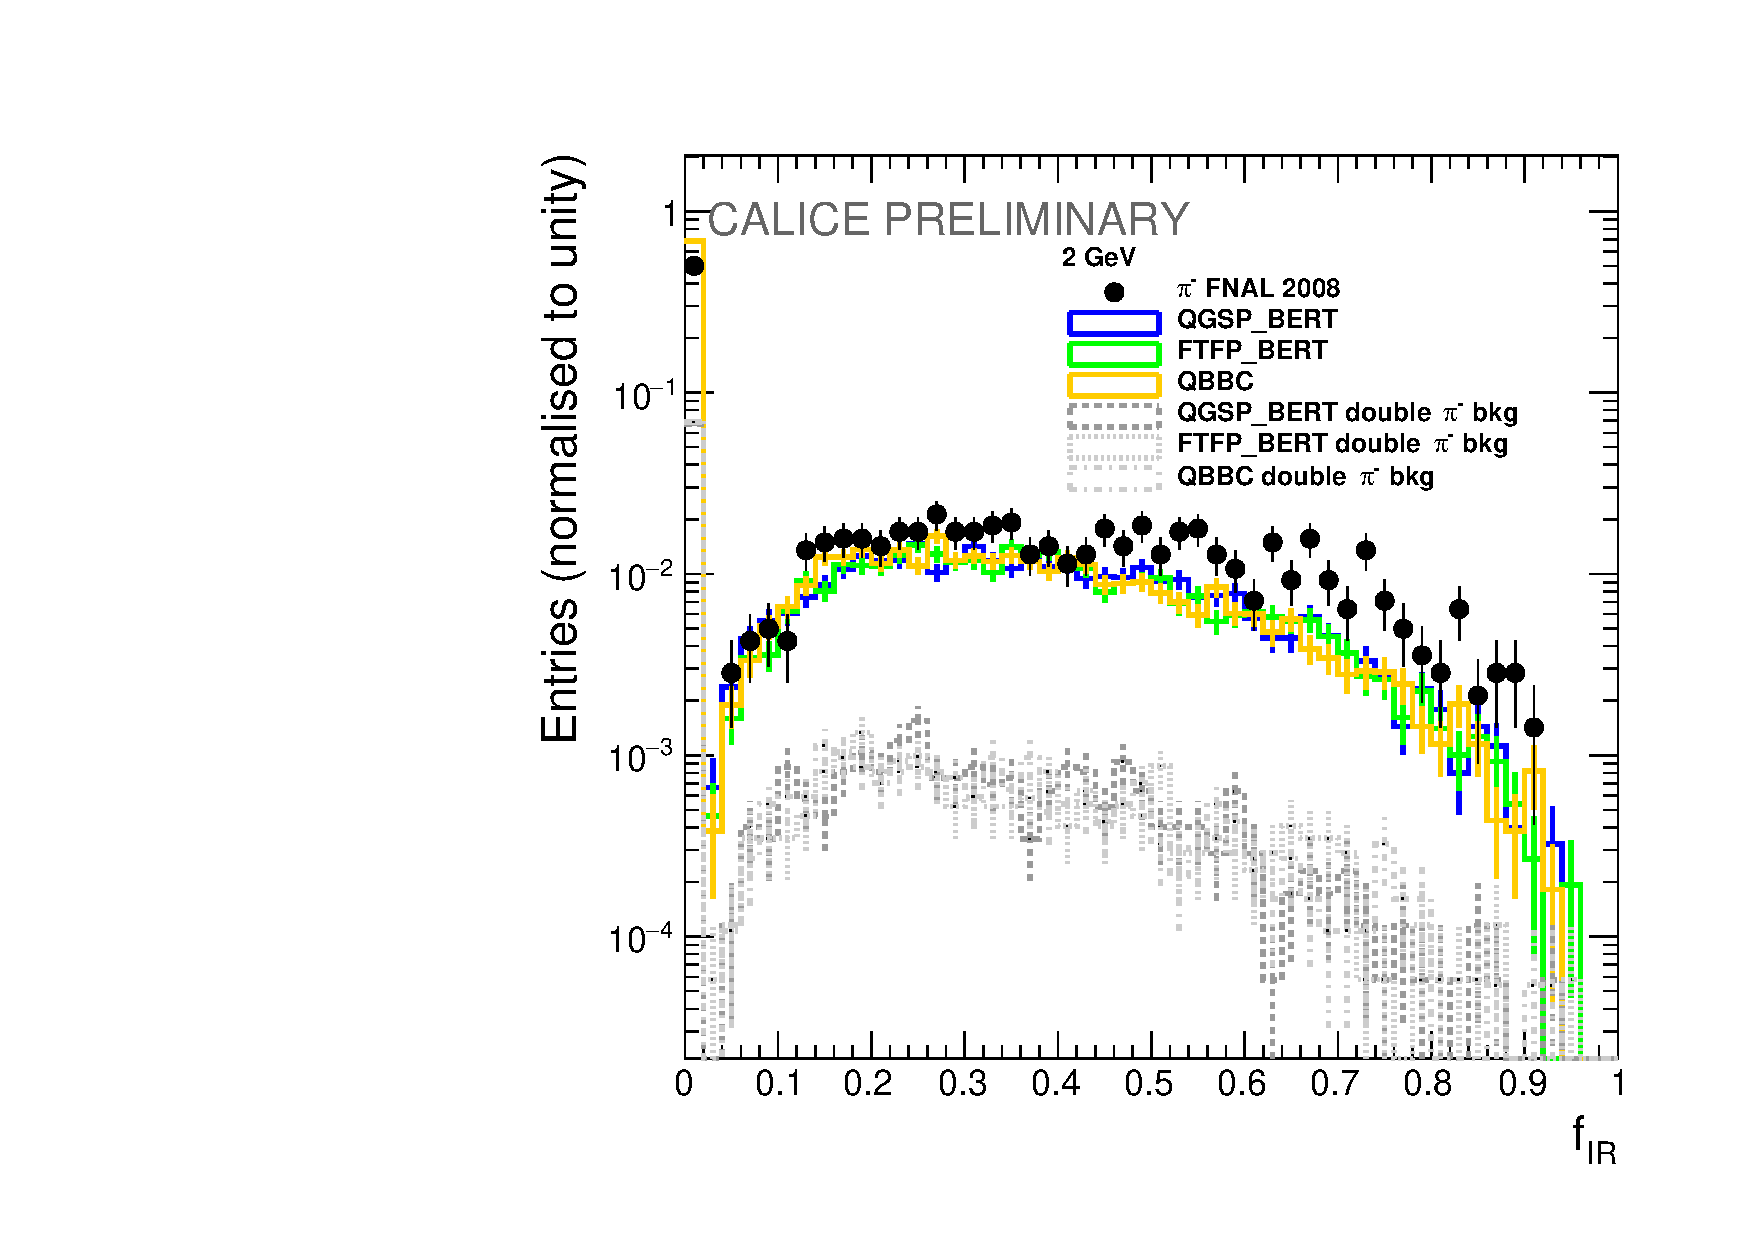
\includegraphics[width=.90\linewidth]{ECAL/plots/e-ir-2.pdf}
		\caption{\label{fig:efr2} }
	\end{subfigure}% 
	\begin{subfigure}{0.5\textwidth}
		\centering
		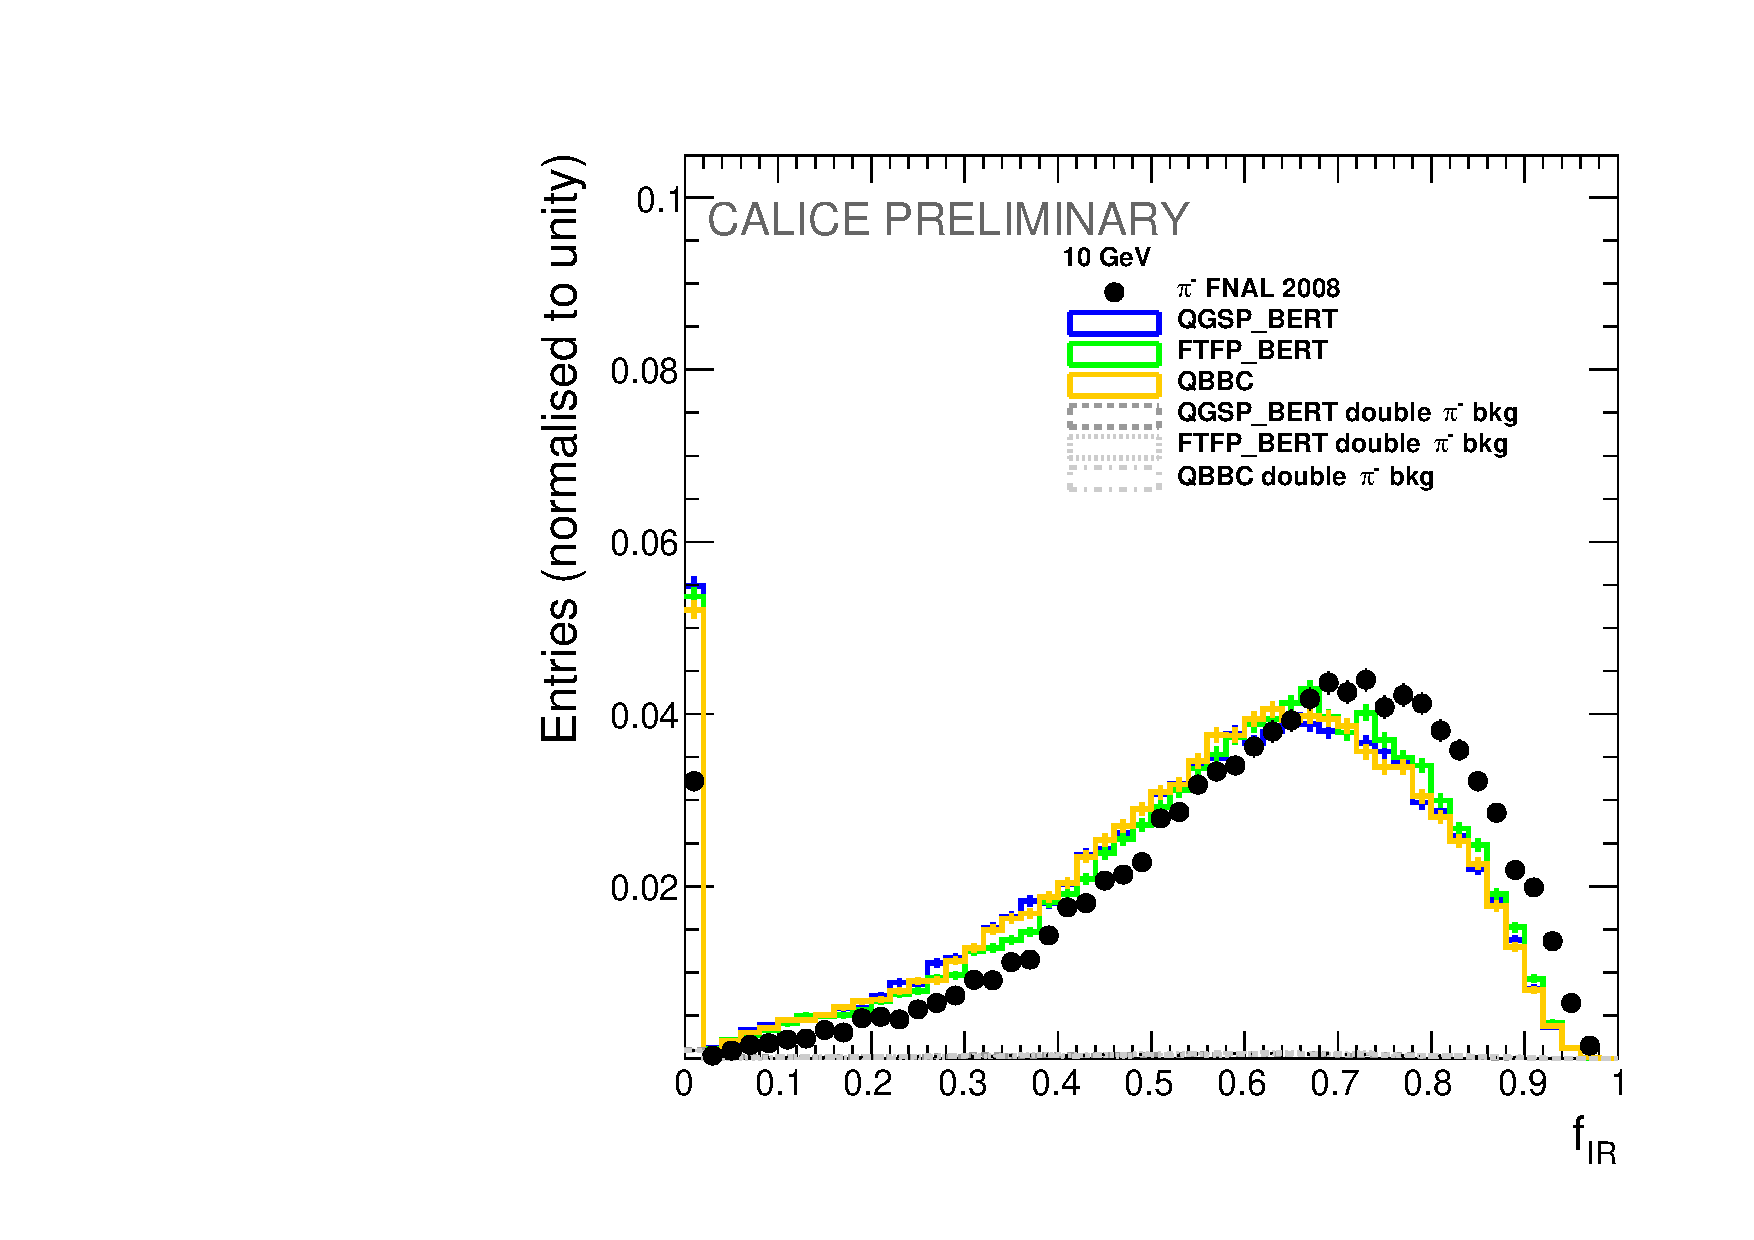
\includegraphics[width=.90\linewidth]{ECAL/plots/e-ir-10.pdf}
		\caption{\label{fig:efr10} }
	\end{subfigure}
	\caption{\label{fig:irexample} \sl {\bf Fig.~\ref{fig:efr2}: Remind me how the linear plot looks like} Comparison of $f_{IR}$ between data and Monte Carlo simulations for two {\sc Geant}4 physics lists for energies of 2 (a) and 10 (b) GeV of the primary particle, respectively. The first bin contains events without a detected interaction region. All histograms are normalised to unity. Error bars represent statistical uncertainties only.}
\end{figure}

\begin{figure}
	\centering
	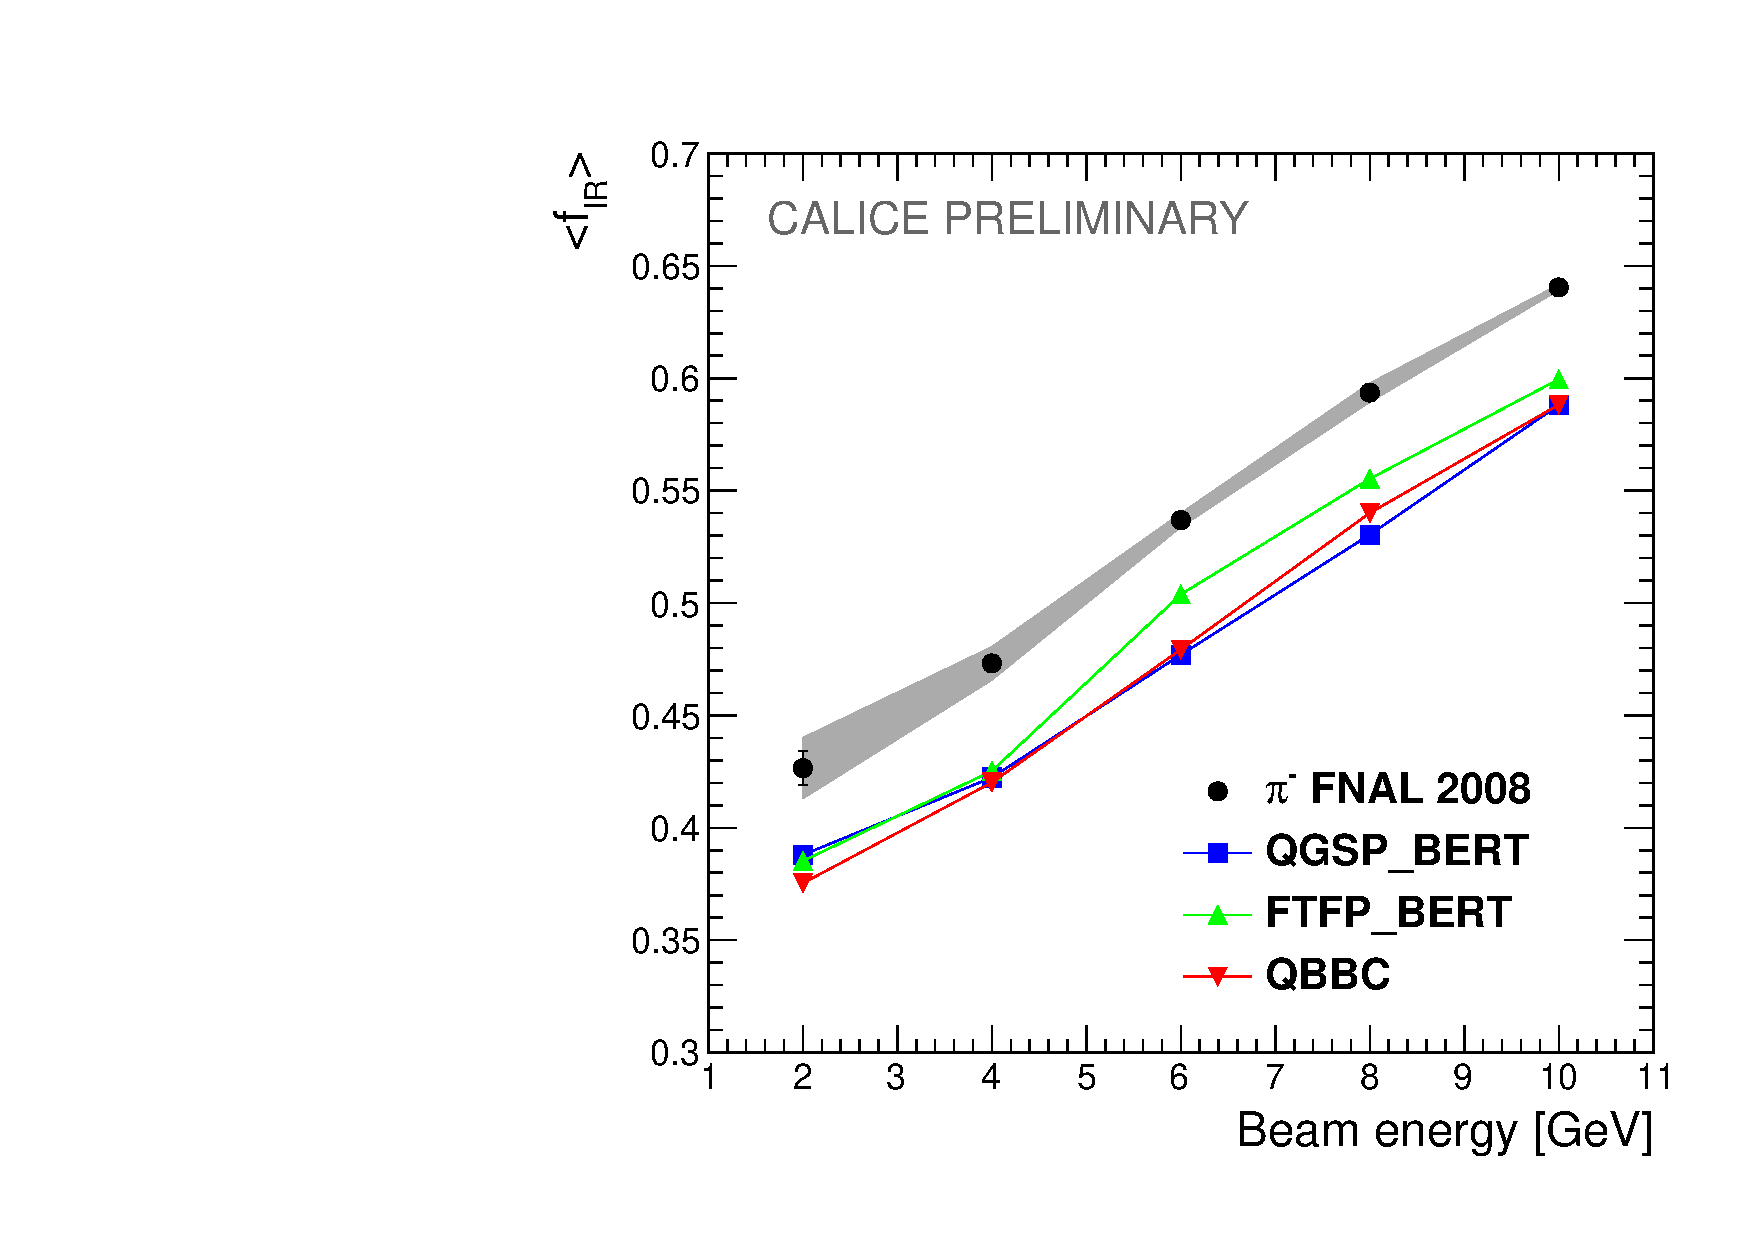
\includegraphics[width=0.5\textwidth]{ECAL/plots/e-ir-graph.pdf}
	\caption{\label{fig:irgraph} \sl  Mean fraction of energy deposition in the interaction region in \ecal\ for data and  Monte Carlo simulations for two {\sc Geant}4 physics lists as a function of the beam energy (2\,GeV to 10\,GeV). Events without a detected interaction region according to Sec.~\ref{sec:iazone} are discarded. The error bars represent statistical uncertainties and the error band the systematic error from the correction for double $\pi$ events.}
\end{figure}
\subsection{Lateral radius of interaction region}
%|||||||||||||||Radius of interaction zone|||||||||||||||||||
%Along with $f_{IR}$, 
The lateral radius $r_{IR}$  of the detected interaction region averaged over hits with respect to the lateral barycentre is a measure of the spatial extension of the interaction region. 
It is defined as:
\begin{equation}
r_{IR} = \frac{\displaystyle \sum_{hit \in IR} \sqrt{(\bar{x}_{IR} - x_{hit})^2 + (\bar{y}_{IR} - y_{hit})^2}} {\displaystyle N_{hits}^{IR}},
\label{eq:rir}
\end{equation}
where the sum runs over the hits in the interaction region, here labeled by $IR$, and $N_{hits}^{IR}$ is the number of hits in the interaction region. In Eq.~\ref{eq:rir} $\bar{x}_{IR}$ and $\bar{y}_{IR}$ are the transversal coordinates of the barycentre of the interaction region that in analogy with Eq.~\ref{eq:barycentre} are defined as: 
\begin{eqnarray}
\label{eq:barycentre2}
\bar{x}_{IR} = \frac{\displaystyle \sum_{hit \in IR} x_{hit}\,E_{hit}}{\displaystyle \sum_{hit \in IR} E_{hit}} 
\text{ and }
\bar{y}_{IR} = \frac{\displaystyle \sum_{hit \in IR} y_{hit}\,E_{hit}}{\displaystyle \sum_{hit \in IR} E_{hit}},
\end{eqnarray}

Distributions of $r_{IR}$ for data and the predictions by the three tested {\sc Geant4} physics lists are displayed in Fig. \ref{fig:rirexample}
for energies of the primary particle of 2\,GeV and 10\,GeV. In both cases the measured interaction region is wider than the predictions by the {\sc Geant}4 physics lists.  
Figure \ref{fig:irrgraph} displays the dependence of the mean $r_{IR}$, $\left<r_{IR}\right>$, on the beam energy for the data and the three {\sc Geant4} physics lists. Here again, events without a detected interaction region according to Sec.~\ref{sec:iazone} are discarded. The lateral size of the interaction region increases with increasing energy of the primary particle. For all tested energies the interaction region measured in data is constantly around 10\% wider than is the case of the {\sc Geant}4 physics lists that lead to identical results. 
%An interpretation of this observation may be that the simulation is lacking energy depositions by secondaries with a comparatively long mean free path length. 

\begin{figure}
	\centering
	\begin{subfigure}{0.5\textwidth}
		\centering
		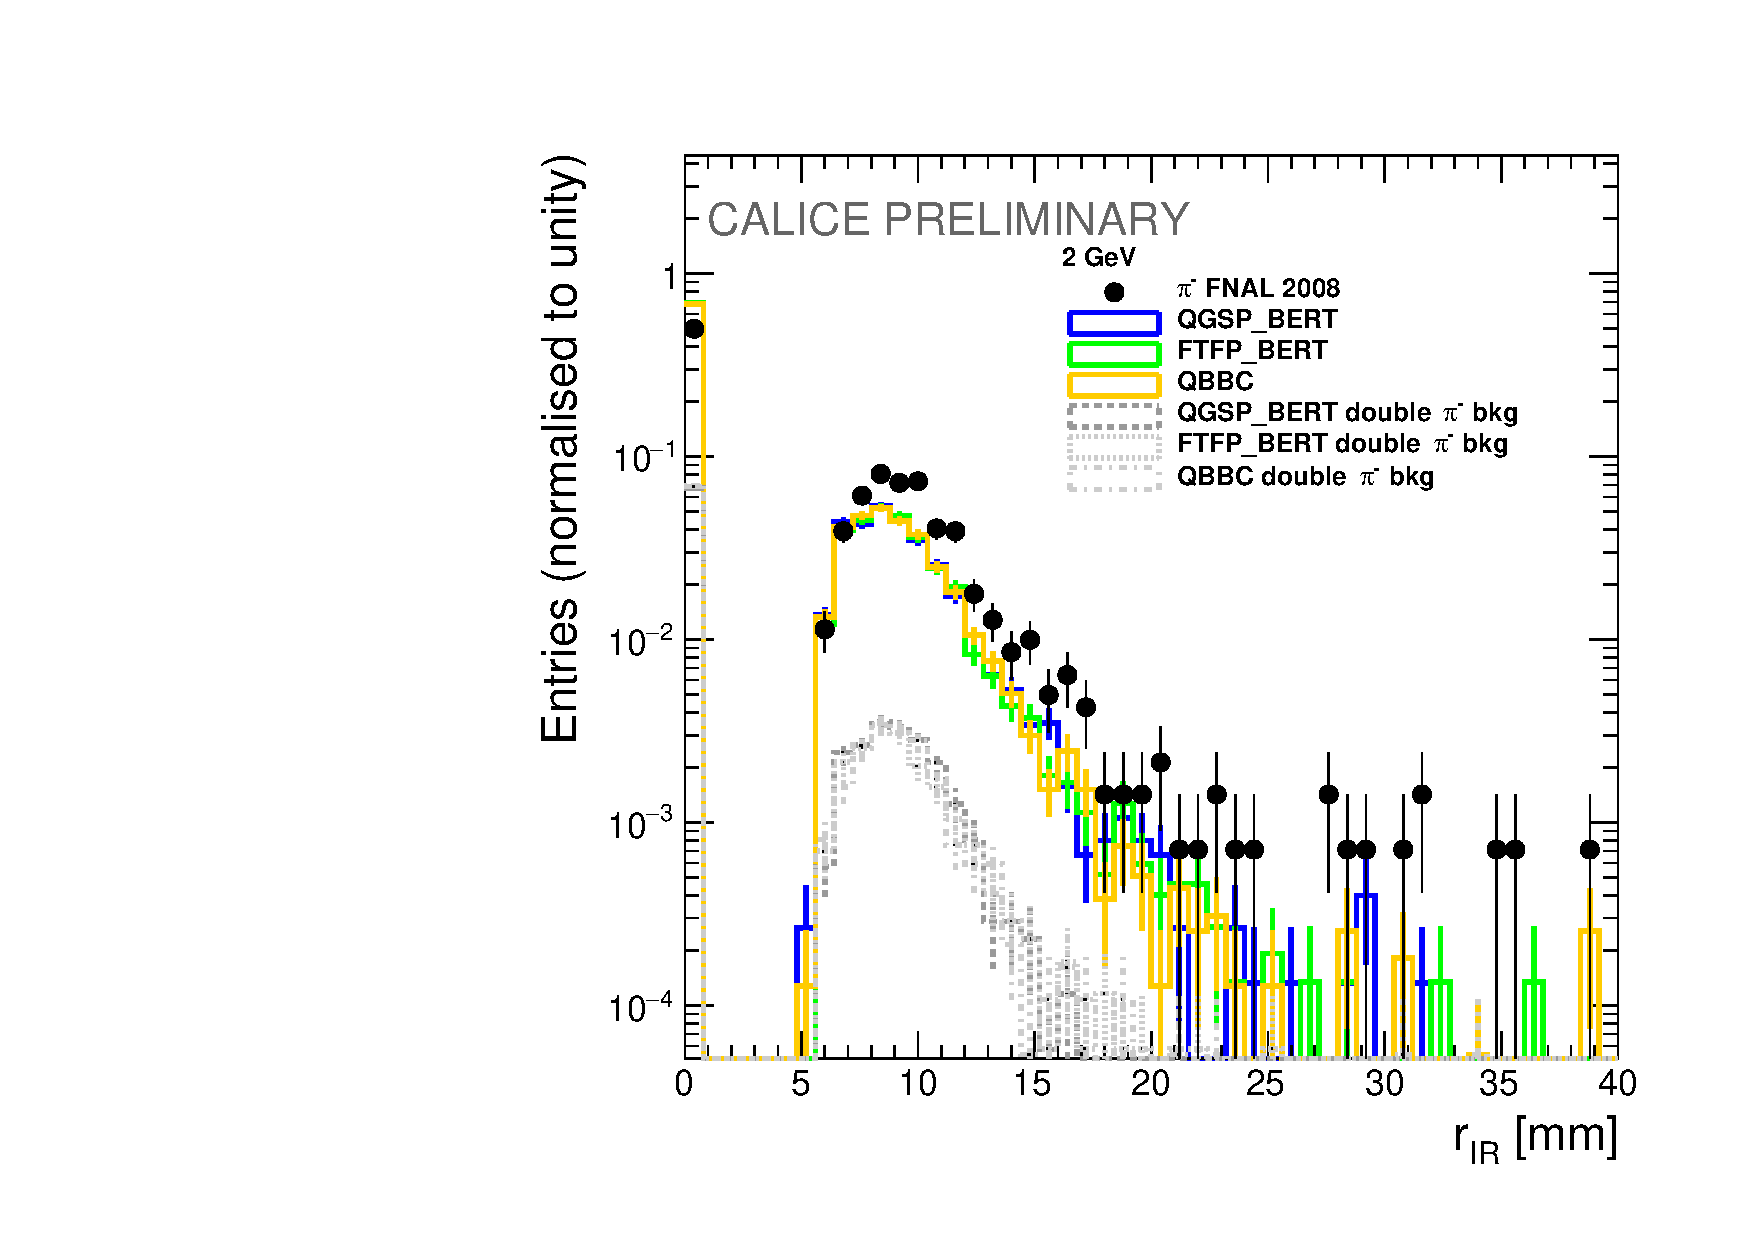
\includegraphics[width=.90\linewidth]{ECAL/plots/r-ir-2.pdf}
		\caption{\label{fig:rir2} }
	\end{subfigure}% 
	\begin{subfigure}{0.5\textwidth}
		\centering
		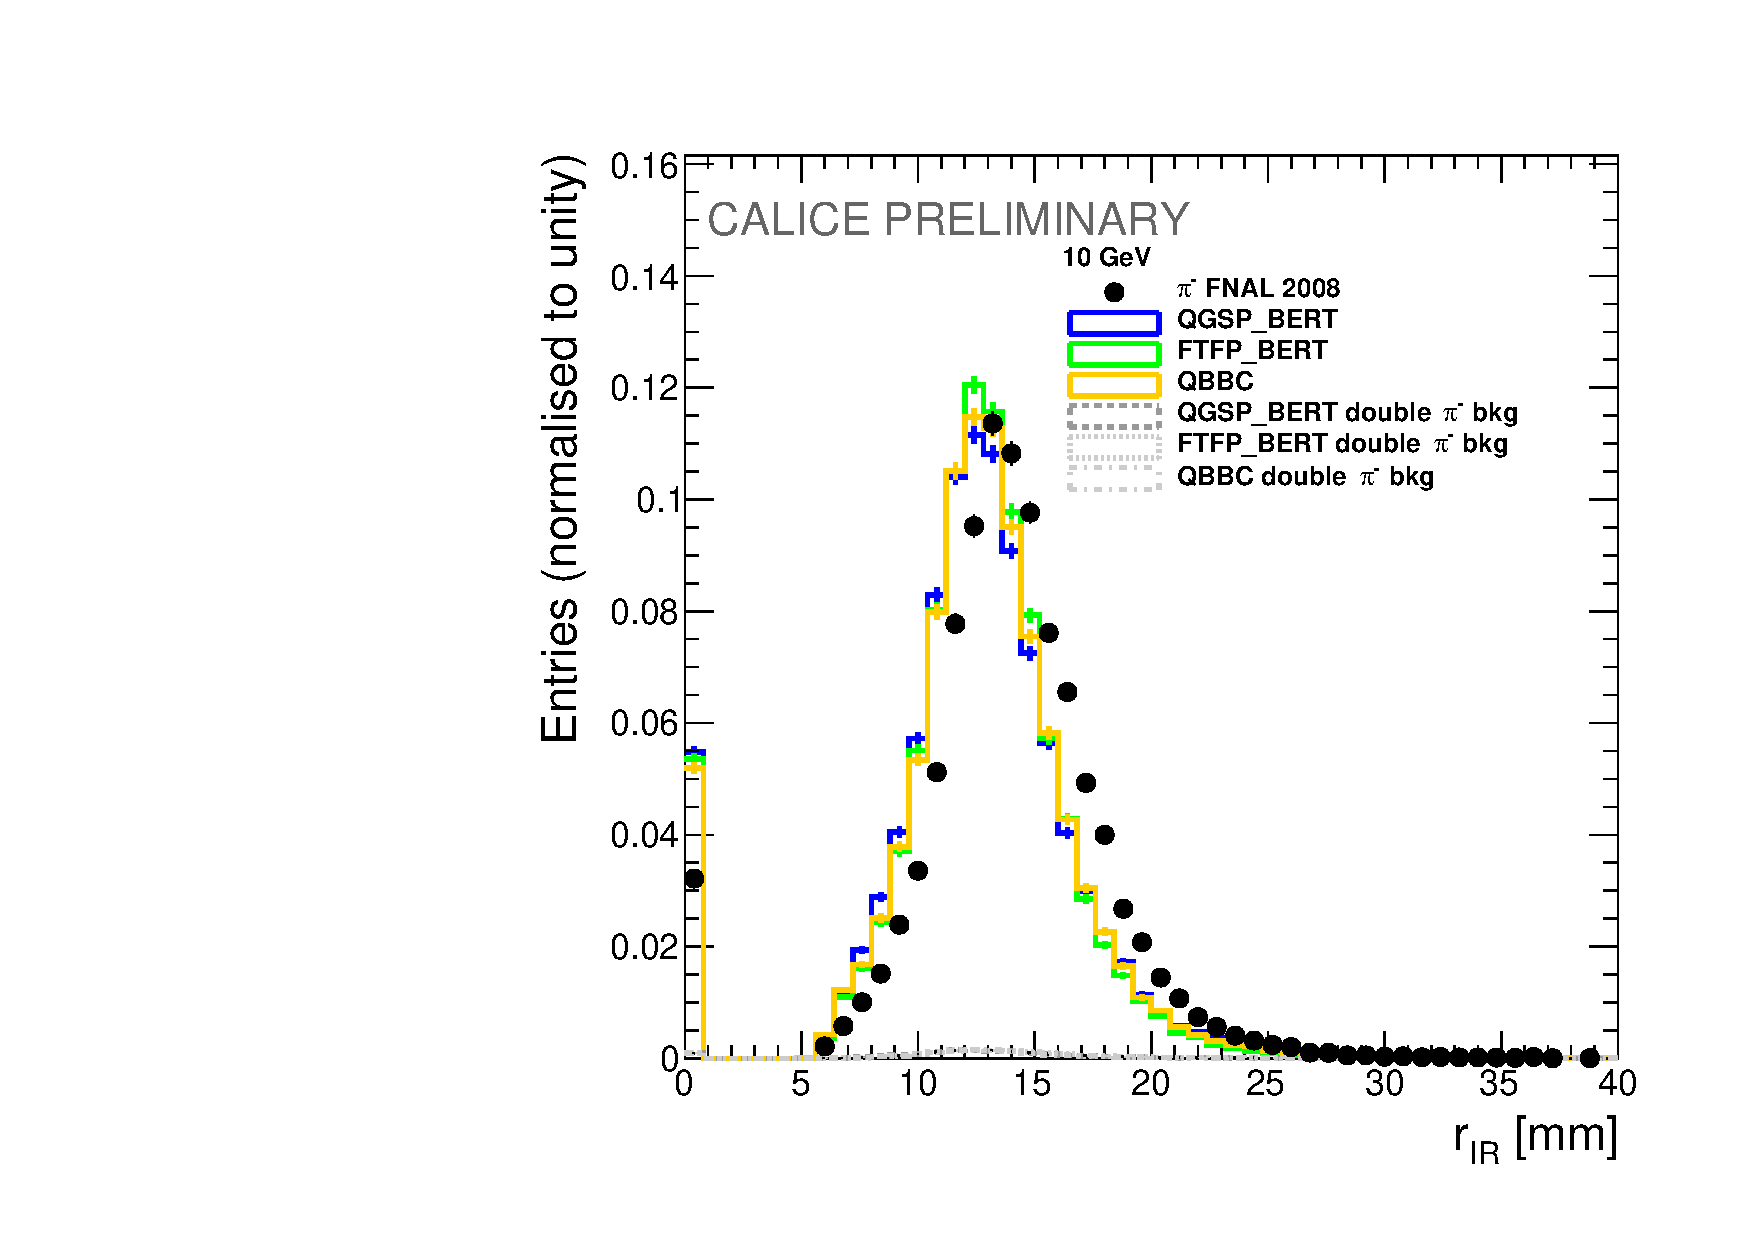
\includegraphics[width=.90\linewidth]{ECAL/plots/r-ir-10.pdf}
		\caption{\label{fig:rir10} }
	\end{subfigure}
	\caption{\label{fig:rirexample} \sl {\bf Same remark as for Fig.~\ref{fig:efr2} } Comparison of $r_{IR}$ distributions for data and Monte Carlo simulations for two {\sc Geant}4 physics lists for energies of the primary particle of 2 (a) and 10 (b) GeV, respectively. All histograms are normalised to unity. Error bars represent statistical uncertainties only.}
\end{figure}

\begin{figure}
	\centering
	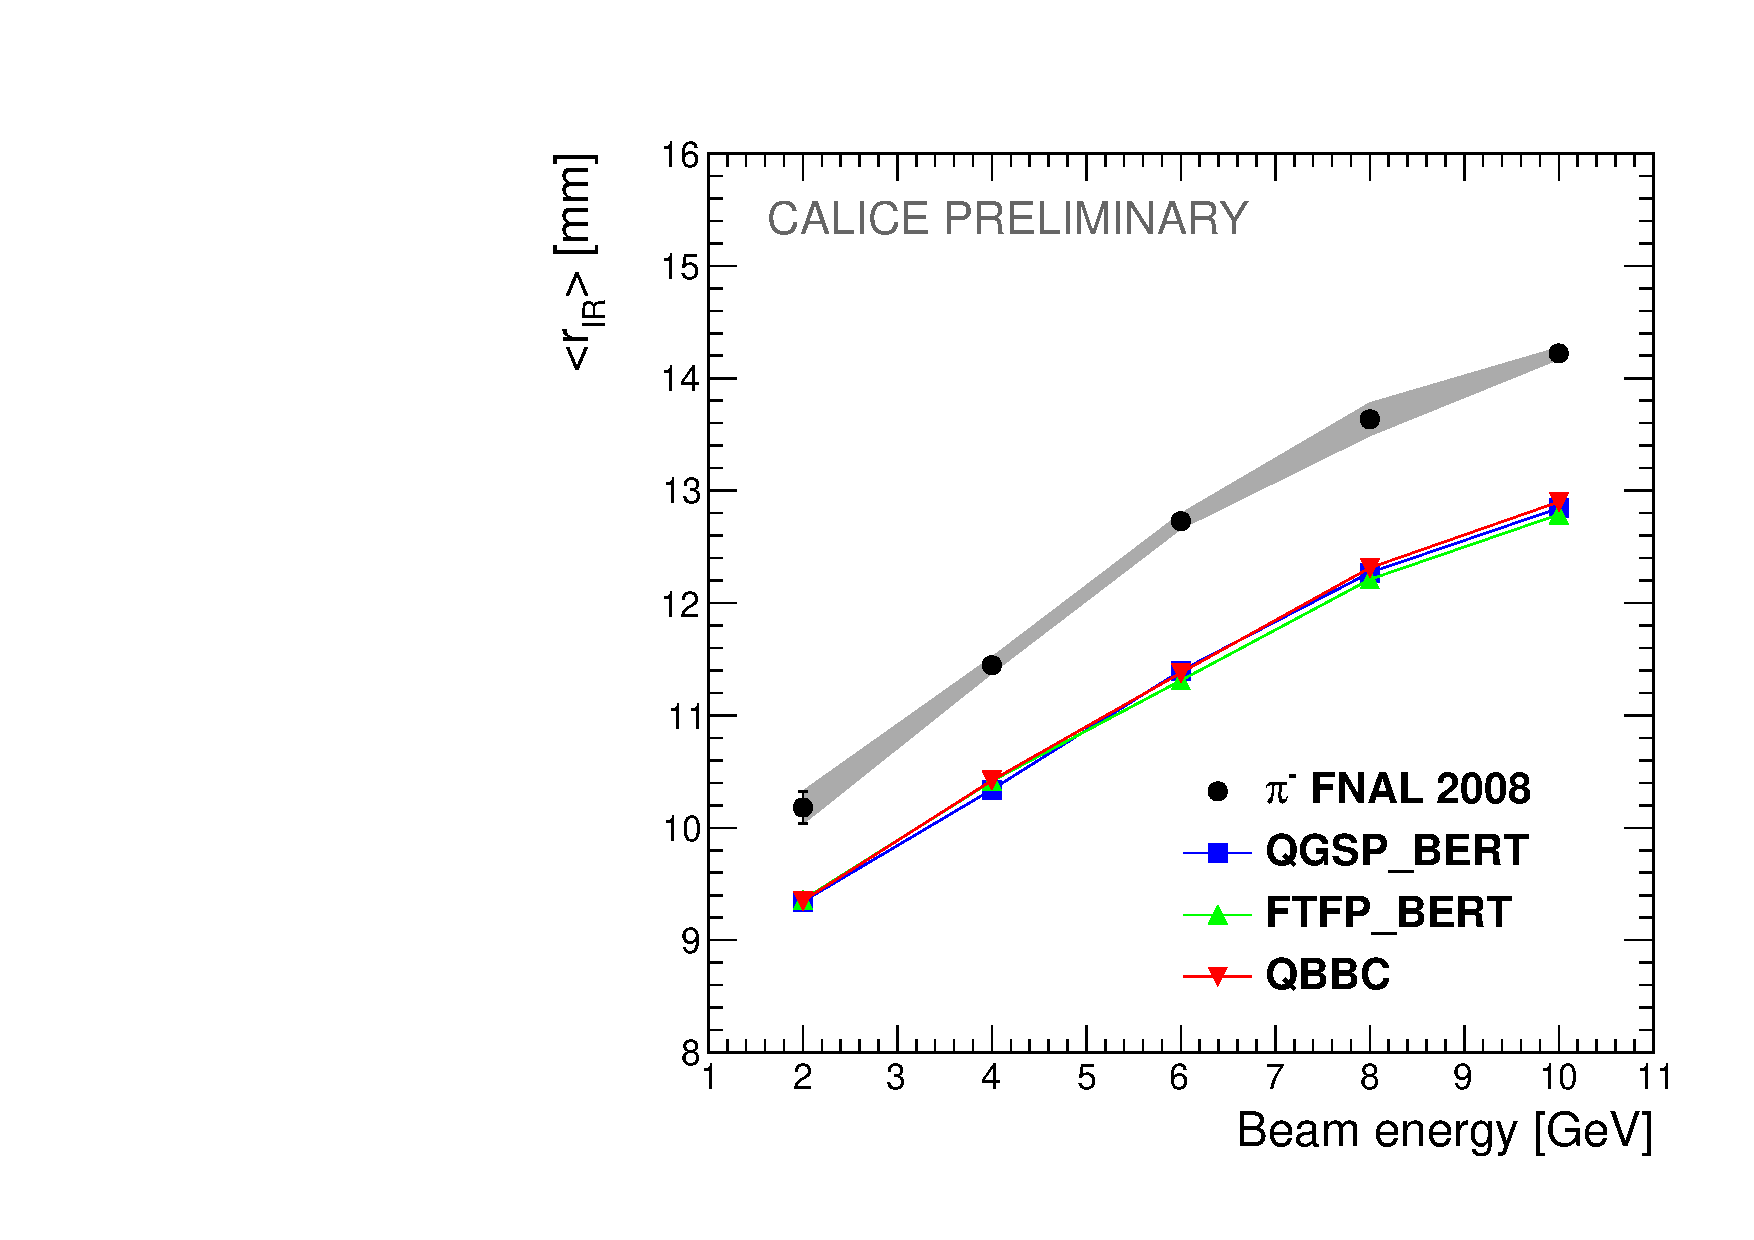
\includegraphics[width=0.5\textwidth]{ECAL/plots/r-ir-graph.pdf}
	\caption{\label{fig:irrgraph} \sl Mean $r_{IR}$ for data and Monte Carlo simulations for two {\sc Geant}4 physics lists as a function of the beam energy. Events without a detected interaction region according to Sec.~\ref{sec:iazone} are discarded. Error bars represent statistical uncertainties only and the error band the systematic error from the correction for double $\pi$ events.}
\end{figure}

%|||||||||||||||||||Number of clusters||||||||||||||||||||||
\subsection{Number of clusters}
As the final tracks are composed from segments that are given by clusters according to Sec.~\ref{sec:cluster}, it is instructive to study the total number of clusters ($N_{clusters}$) detected by the \tfa\ in the event. This observable is stable against details of the \tfa\,
since it does not depend neither on the \ep\ value nor on other free parameters of the classification algorithm. Here and in all of the following events without a detected interaction region according to Sec.~\ref{sec:iazone} are discarded.
The $N_{clusters}$ distribution is given in Fig. \ref{fig:clusterexample} for data and Monte Carlo simulation for the three {\sc Geant4} physics lists for energies of 2 and 10\,GeV of the incoming $\pi^-$-meson, respectively. The measured distributions are slightly shifted towards higher values with respect to those obtained for the three {\sc Geant4} physics lists.
%While the data and MC agree in many bins within errors, the distributions are nevertheless slightly shifted w.r.t. each other.  

Figure \ref{fig:clustergraph} shows the dependence of $\left<N_{clusters}\right>$  on different beam energies for data, \ftfp\ and \qgsp\ Monte Carlo simulations. At all energies the data are systematically above the Monte Carlo predictions with deviations of up to 7\%. The agreement tends to improves with increasing energy of the primary particle and is best at 10\,GeV. 
%At 2 and 10\,GeV there is a good agreement between data and both simulation samples, but for intermediate beam energies the \tfa\ tends to find more clusters in data than in Monte Carlo.
\begin{figure}
	\centering
	\begin{subfigure}{0.5\textwidth}
		\centering
		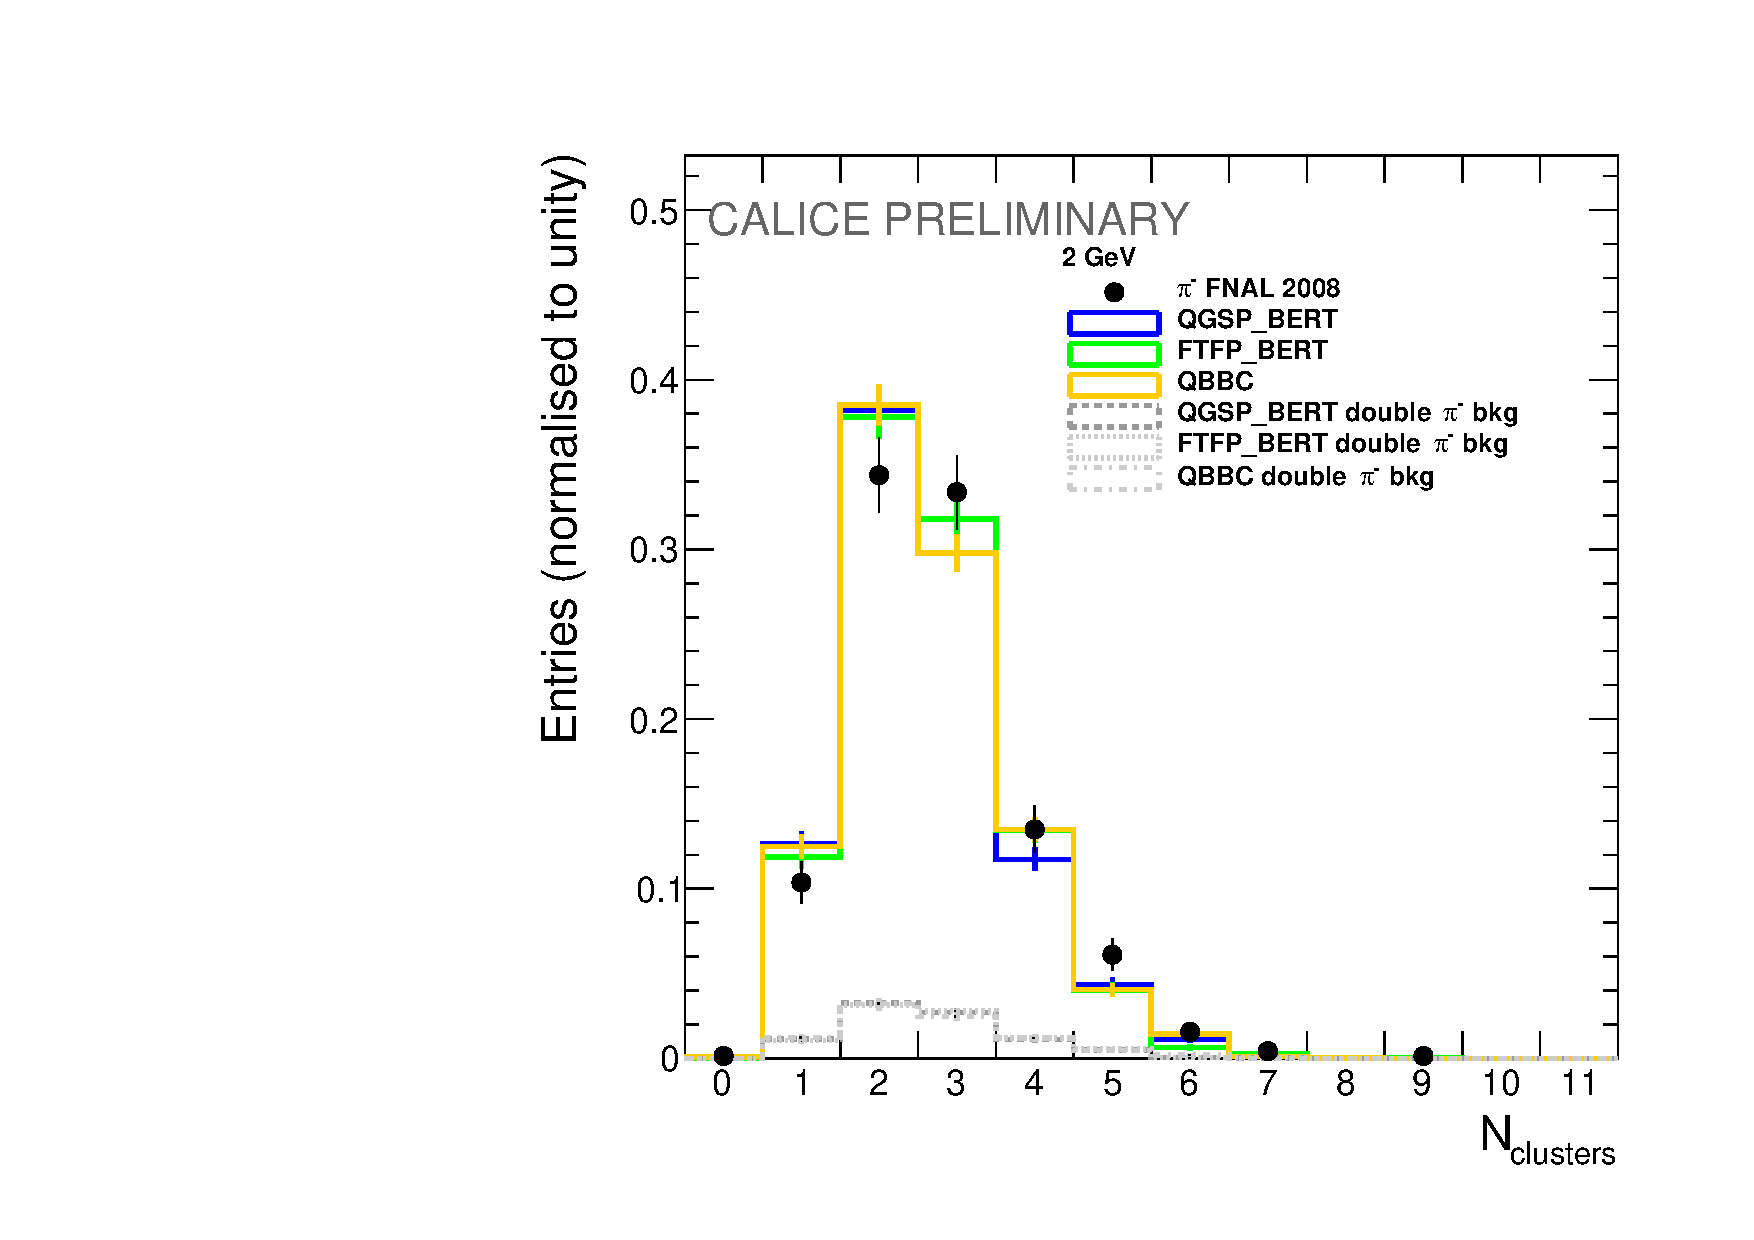
\includegraphics[width=.90\linewidth]{ECAL/plots/cluster-2.pdf}
		\caption{\label{fig:cl2} }
	\end{subfigure}% 
	\begin{subfigure}{0.5\textwidth}
		\centering
		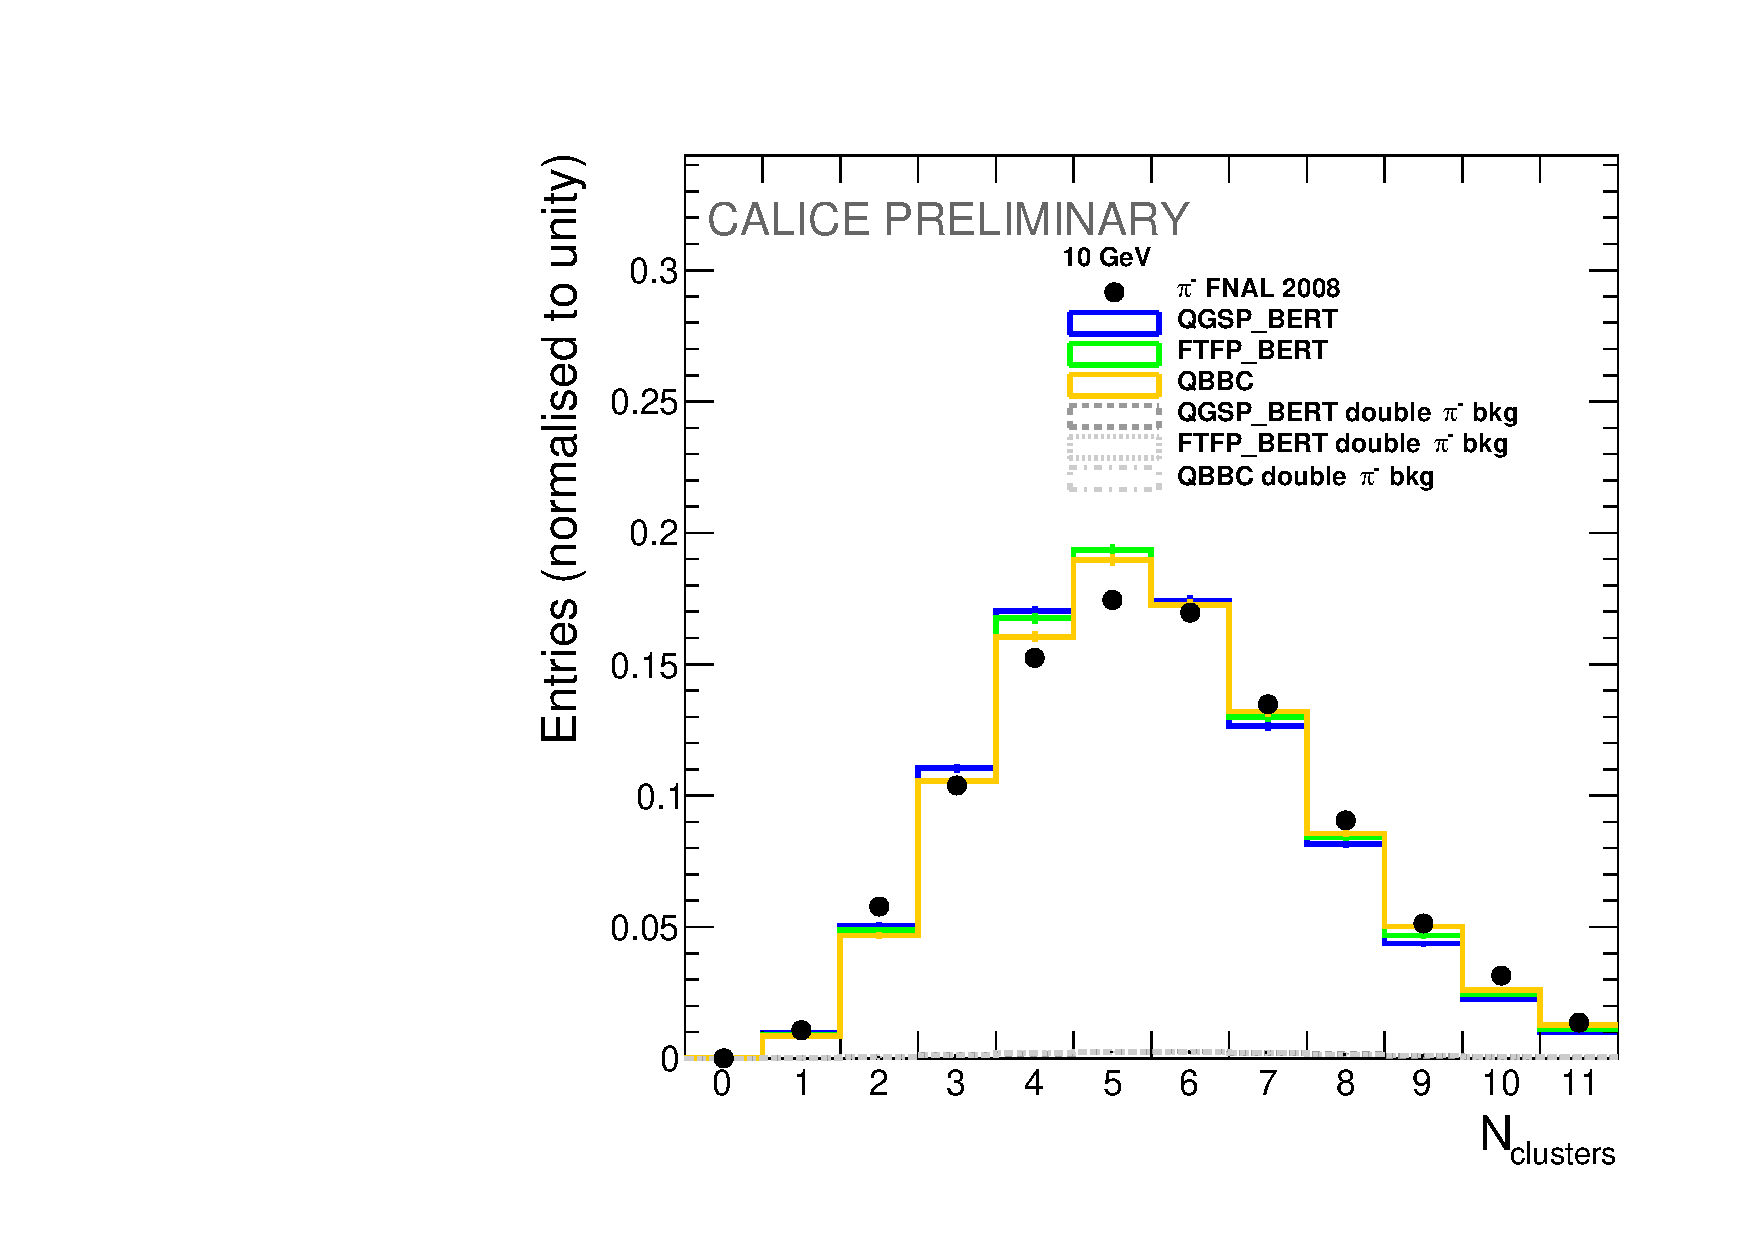
\includegraphics[width=.90\linewidth]{ECAL/plots/cluster-10.pdf}
		\caption{\label{fig:cl10} }
	\end{subfigure}
	\caption{\label{fig:clusterexample} \sl Comparison of the number of clusters found between data and Monte Carlo simulations for two {\sc Geant}4 physics lists for energies of the primary particle of 2 (a) and 10 (b) GeV, respectively. Events without a detected interaction region according to Sec.~\ref{sec:iazone} are discarded. Error bars represent statistical uncertainties only.}
\end{figure}

\begin{figure}
	\centering
	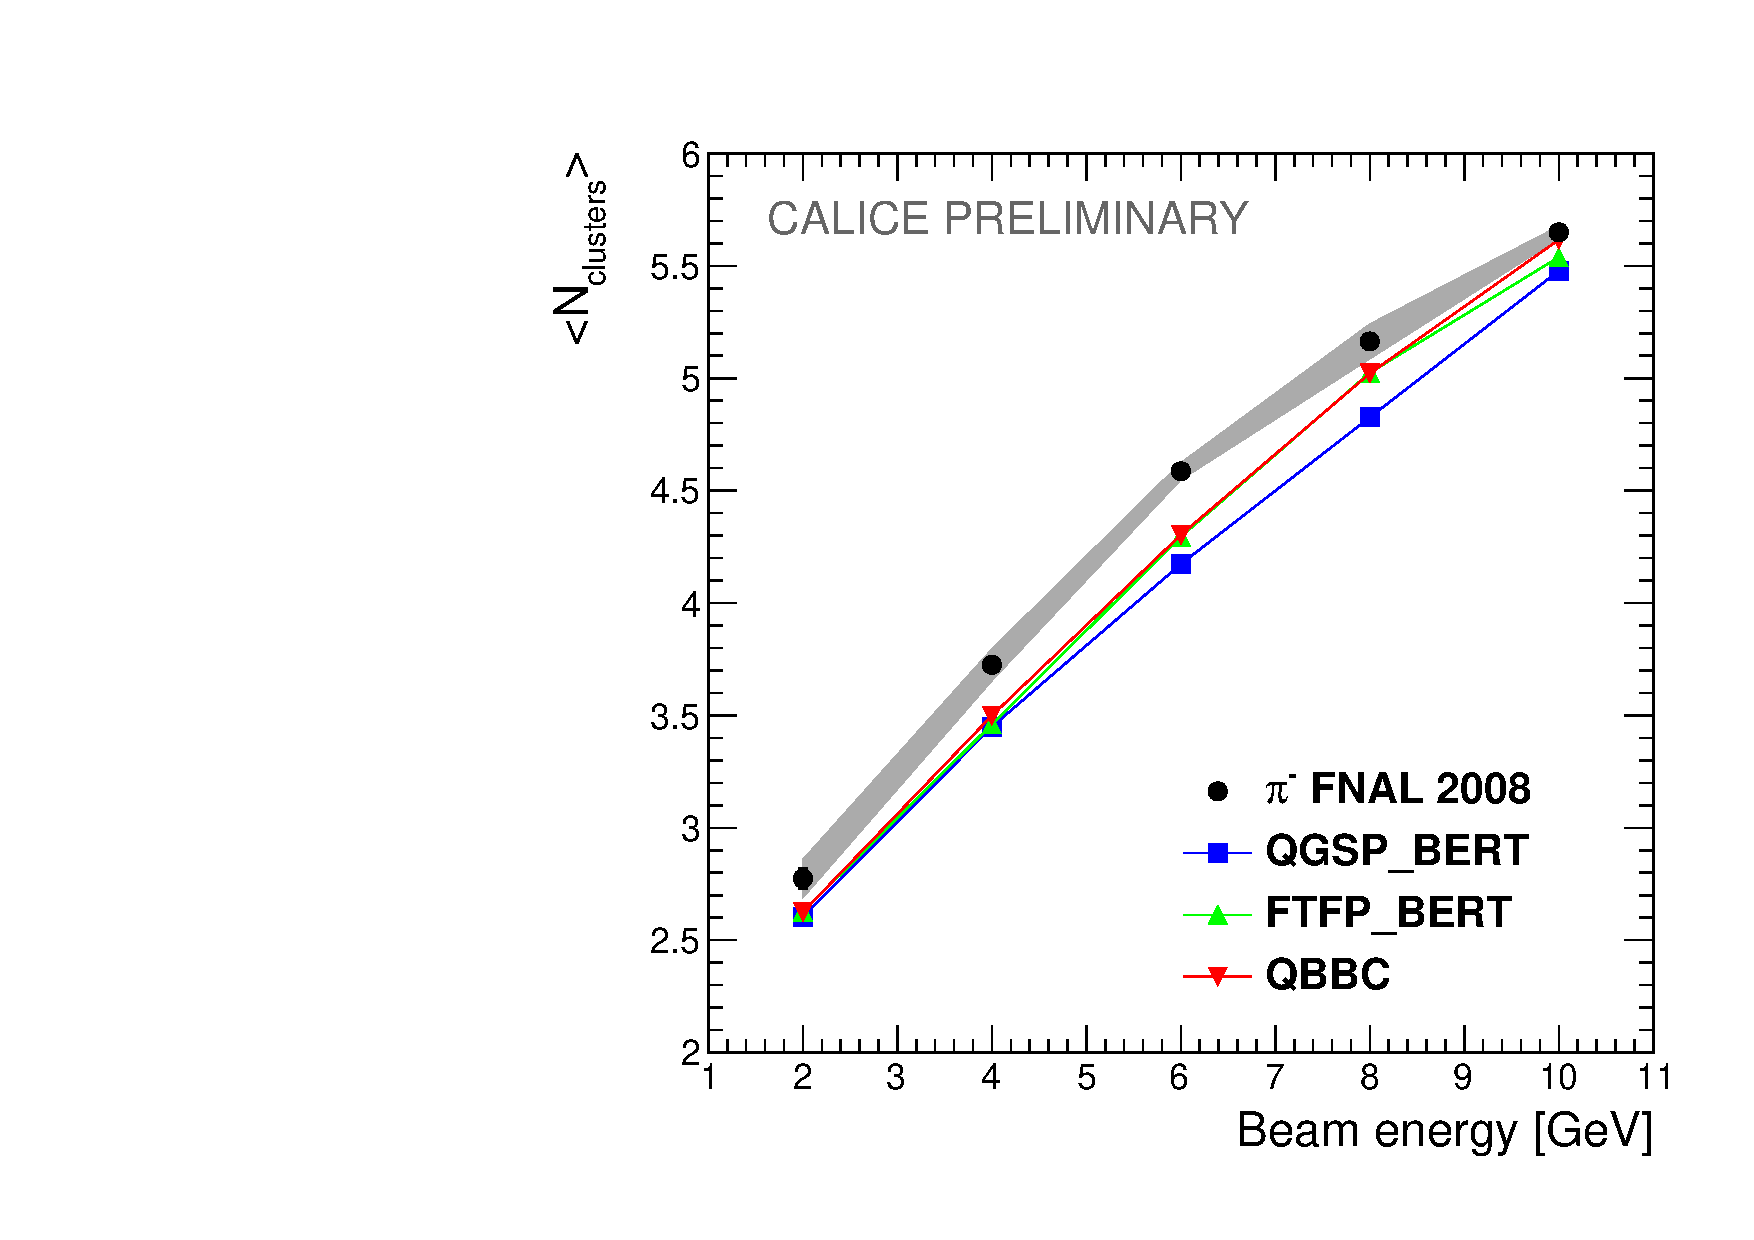
\includegraphics[width=0.5\textwidth]{ECAL/plots/cluster-graph.pdf}
	\caption{\label{fig:clustergraph} \sl Mean number of clusters in the \ecal\ for data and  Monte Carlo simulations for two {\sc Geant}4 physics lists as a function of beam energy (2\,GeV to 10\,GeV). Events without a detected interaction region according to Sec.~\ref{sec:iazone} are discarded. Error bars on the graph represent statistical uncertainties and the error band the systematic error from the correction for double $\pi$ events.}
\end{figure}

%||||||||||||||||||||Number of tracks||||||||||||||||||||||||
\subsection{Number of tracks}
A central result of the \tfa\ is the number of secondary tracks ($N_{tracks}$) and observables based on their properties.
The $N_{tracks}$ distributions are given in Fig. \ref{fig:trackexample} for data and Monte Carlo simulations based on the three tested {\sc Geant4} physics lists for energies of 2 and 10\,GeV of the incoming $\pi^-$-mesons. A remarkably good agreement between data and both physics lists can be reported, given the fact that this observable is analysed for the first time in the \ecal. 

Figure \ref{fig:tracksgraph} shows the dependence of $\left<N_{tracks}\right>$ on the beam energy for data and the three {\sc Geant4} physics lists. 
Both physics lists, presented in Fig.  \ref{fig:tracksgraph} underestimate the number of secondary tracks by 7\% on average below 10\,GeV and are in agreement with the data at 10\,GeV. 
%Both simulation samples are in agreement with data within systematic uncertainties here given by the variation of the \ep\ according to $\varepsilon = 0.03 \pm 0.01$.

%As a measure for the sensitivity of the reconstructed number of tracks on the actual value of the \ep, the estimator 
%\begin{equation}
%\Delta {\cal O} = < {\cal O}(\varepsilon_{up}) - {\cal O}(\varepsilon_{low}> /{\cal O}(\varepsilon_{nom} = 0.03)>
%\end{equation}
%is introduced
The sensitivity to the \ep\ defined by Eq.~\ref{eq:sens} for ${\cal O}=N_{tracks}$, $\varepsilon_{1},=0.04$, $\varepsilon_{2},=0.02$ and $\varepsilon_{nom.}=0.03$   
%$\Delta N_{tracks} = <N_{tracks}(\varepsilon = 0.04) - N_{tracks}(\varepsilon = 0.02)> /<N_{tracks}(\varepsilon = 0.03)> $ is used. 
is shown in Fig. \ref{fig:dtracksgraph}. Within the chosen range the number of reconstructed tracks varies by about 10\% for both, data and the three {\sc Geant4} physics lists. 
\begin{figure}
	\centering
	\begin{subfigure}{0.5\textwidth}
		\centering
		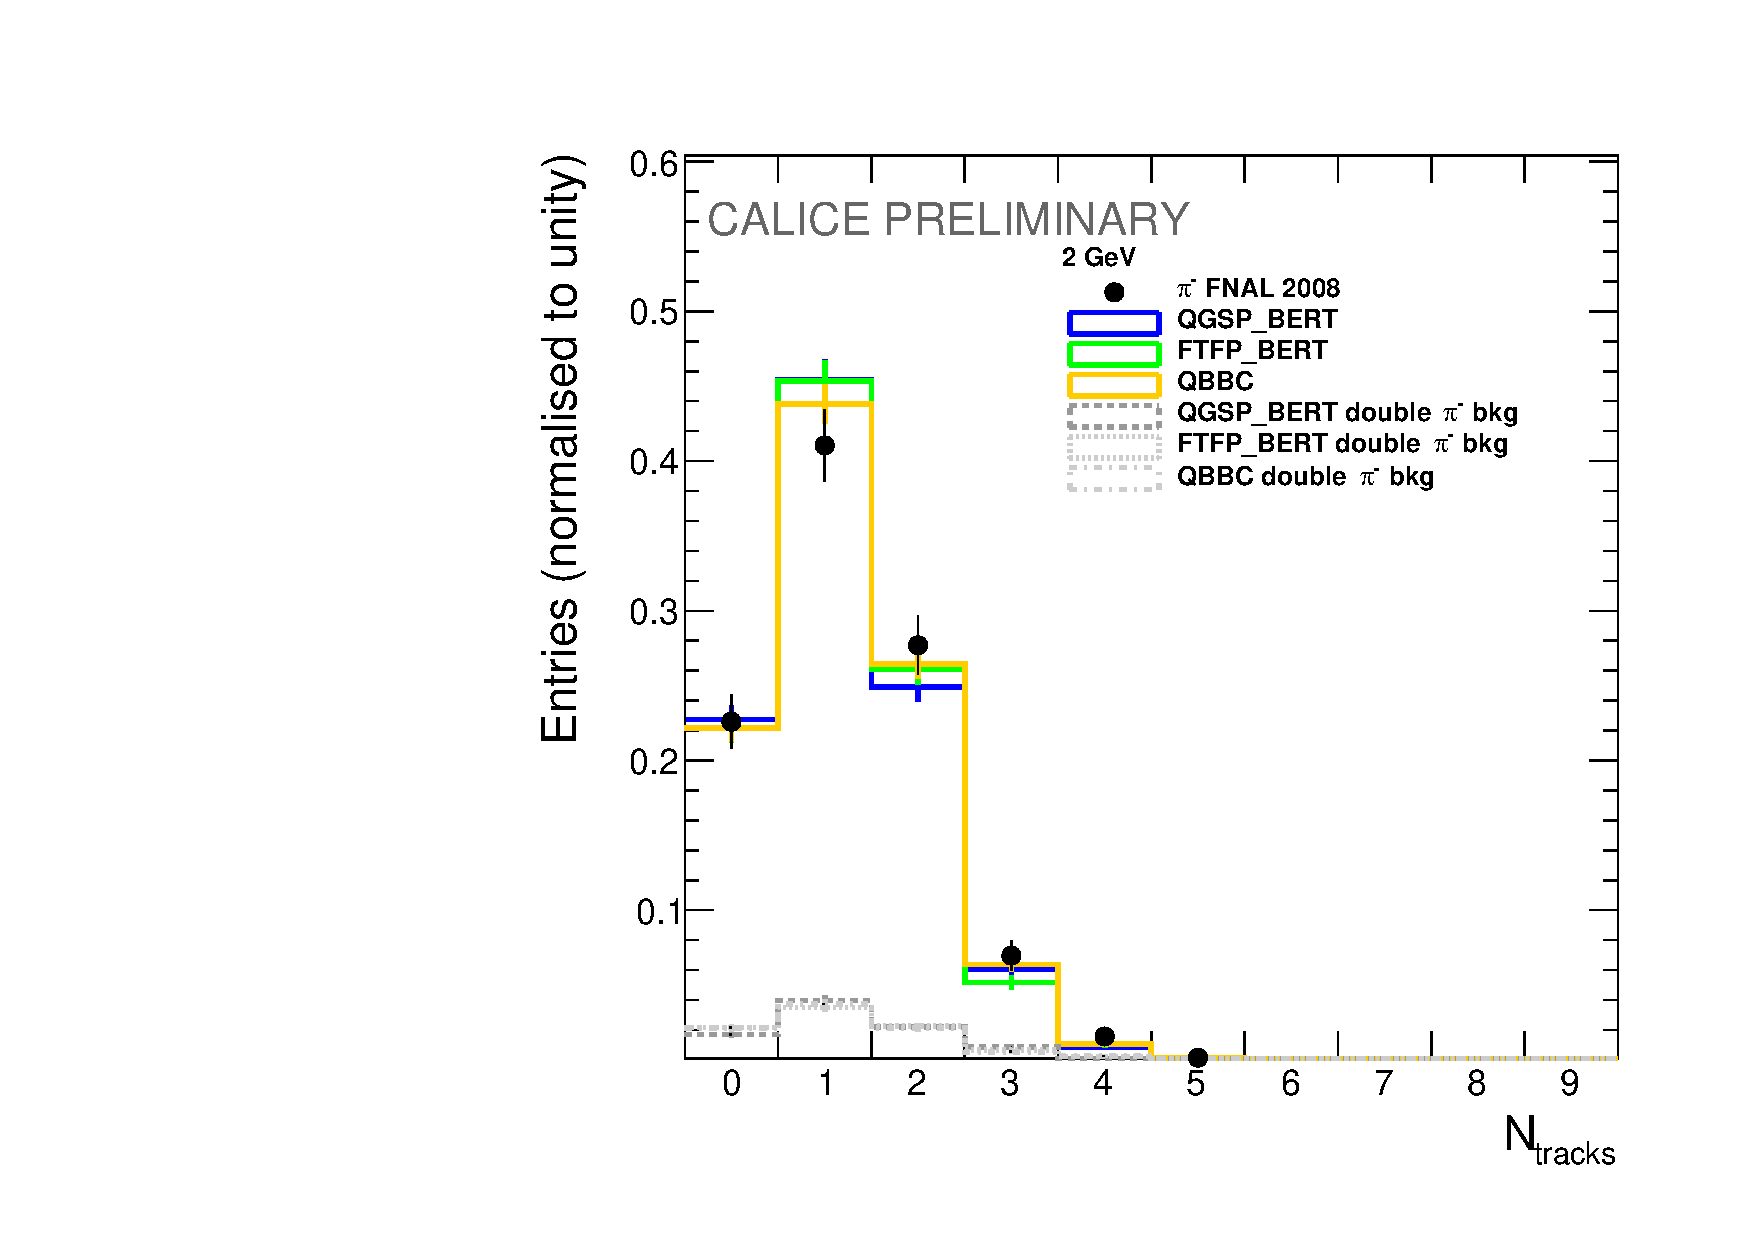
\includegraphics[width=.90\linewidth]{ECAL/plots/ntracks-2.pdf}
		\caption{\label{fig:tr2} }
	\end{subfigure}% 
	\begin{subfigure}{0.5\textwidth}
		\centering
		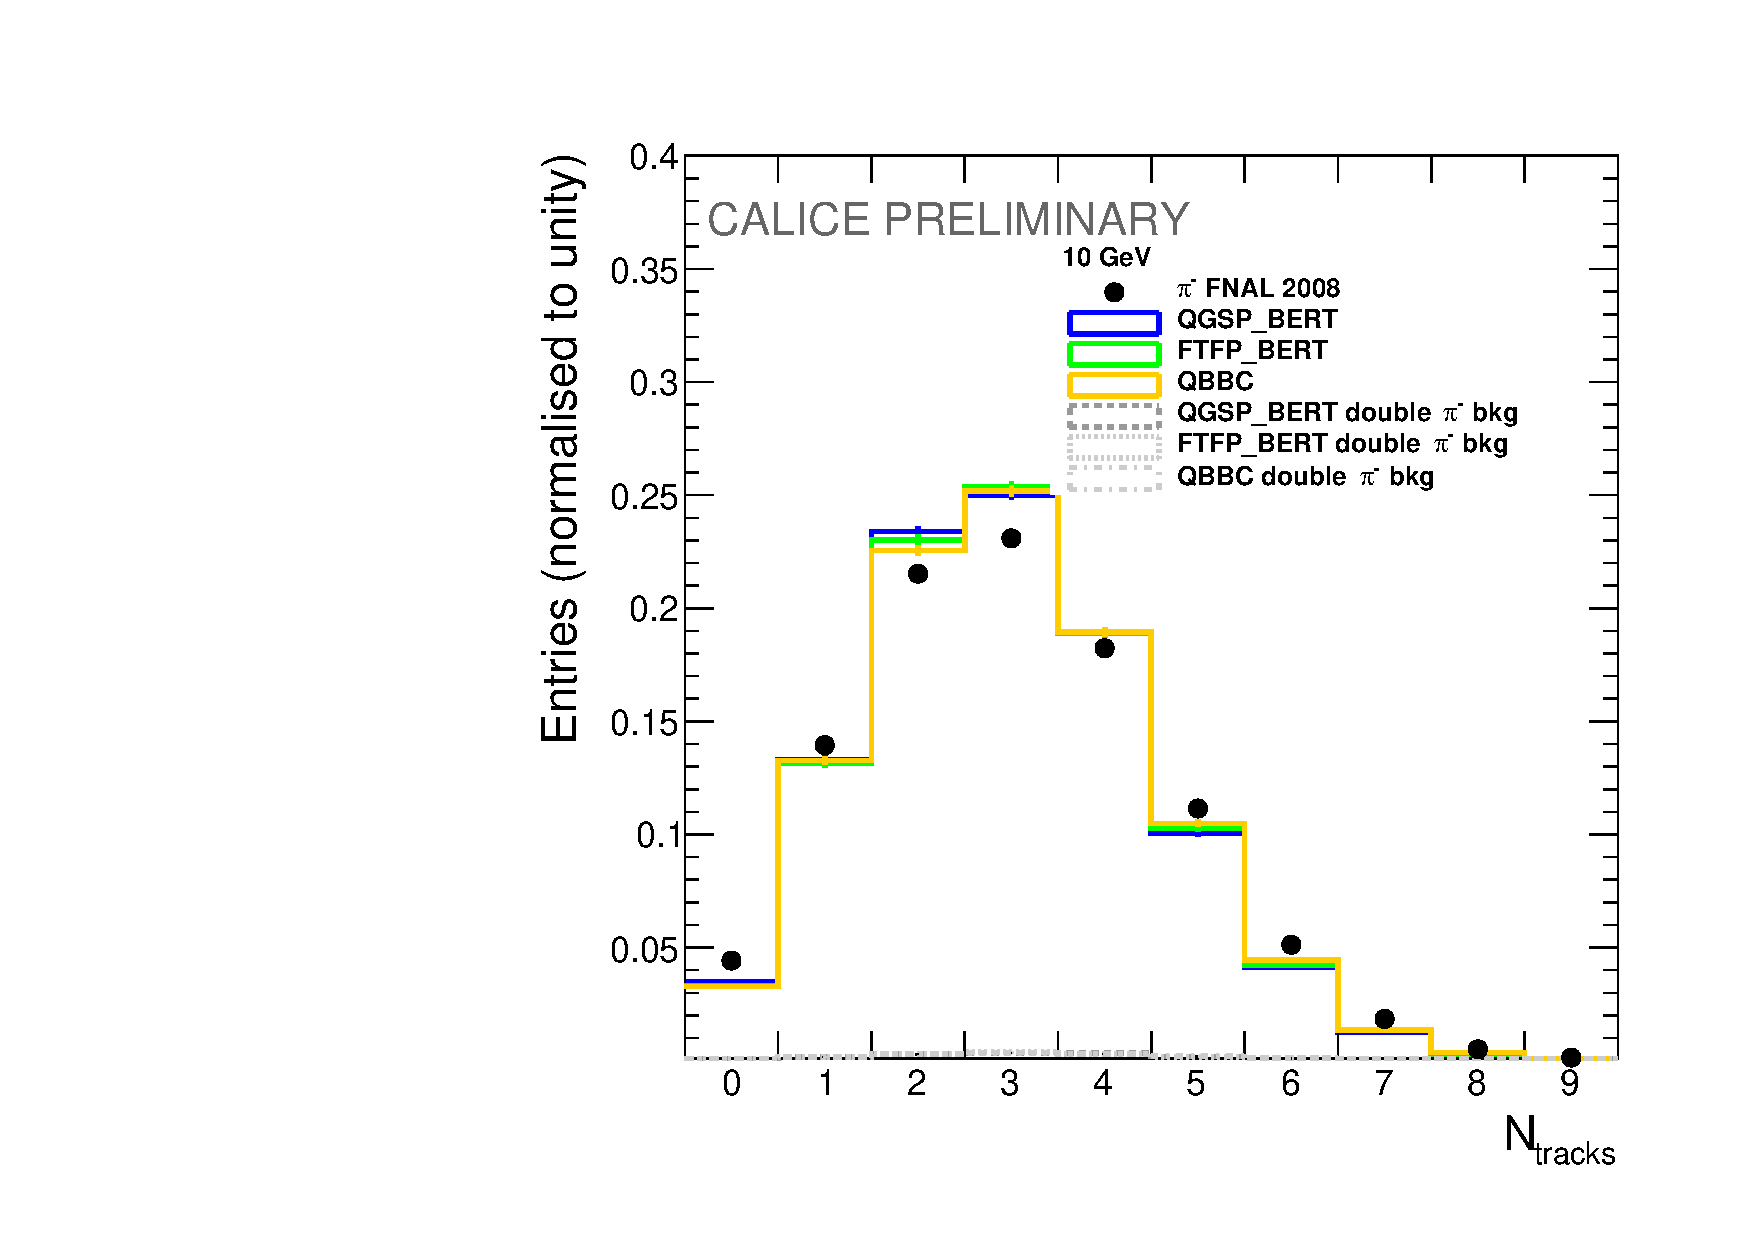
\includegraphics[width=.90\linewidth]{ECAL/plots/ntracks-10.pdf}
		\caption{\label{fig:tr10} }
	\end{subfigure}
	\caption{\label{fig:trackexample} \sl Comparison of the number of secondary tracks between data Monte Carlo simulations for two {\sc Geant}4 physics lists  for energies of the primary particle of 2 (a) and 10 (b) GeV. Events without a detected interaction region according to Sec.~\ref{sec:iazone} are discarded. Error bars represent statistical errors only.}
\end{figure}

\begin{figure}
	\centering
	\begin{subfigure}{0.5\textwidth}
		\centering
		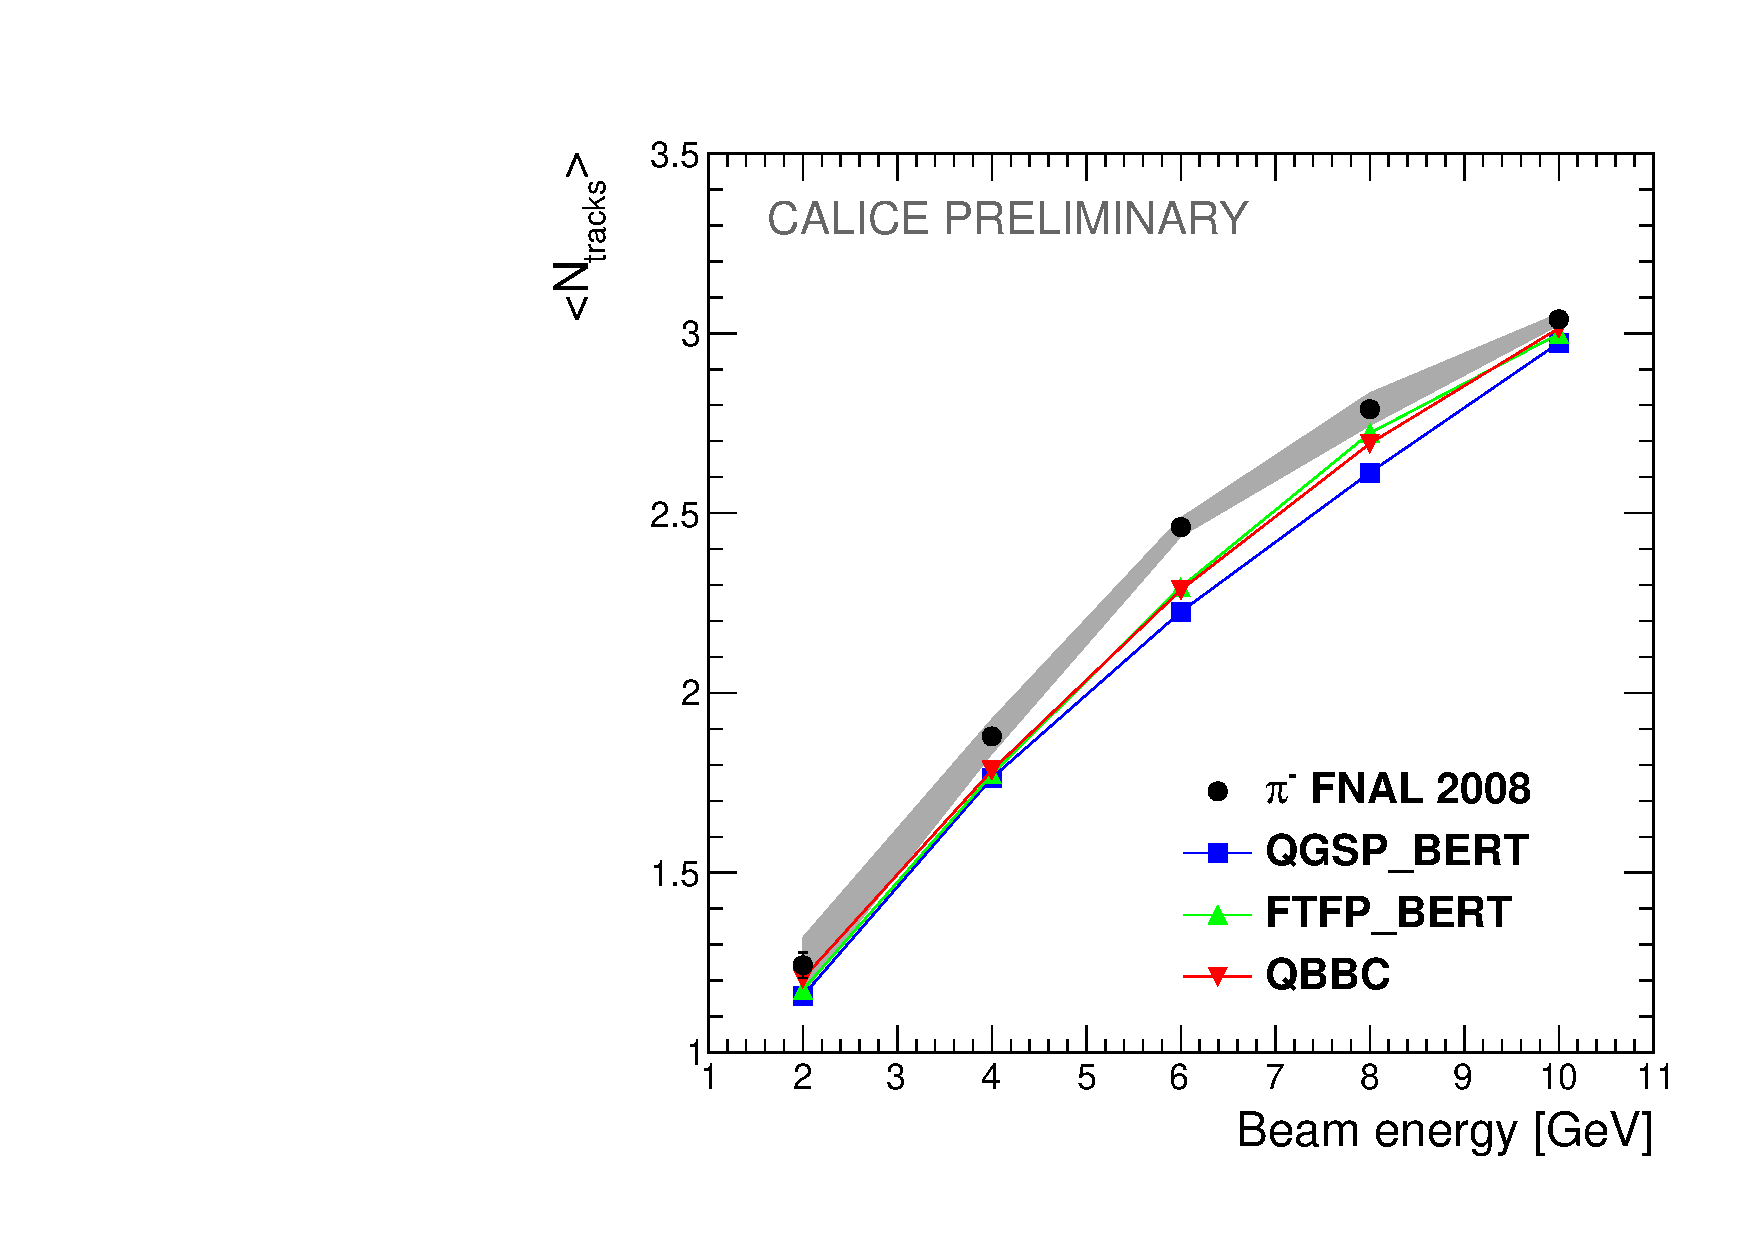
\includegraphics[width=.90\linewidth]{ECAL/plots/ntracks-graph.pdf}
		\caption{\label{fig:tracksgraph} }
	\end{subfigure}% 
	\begin{subfigure}{0.5\textwidth}
		\centering
		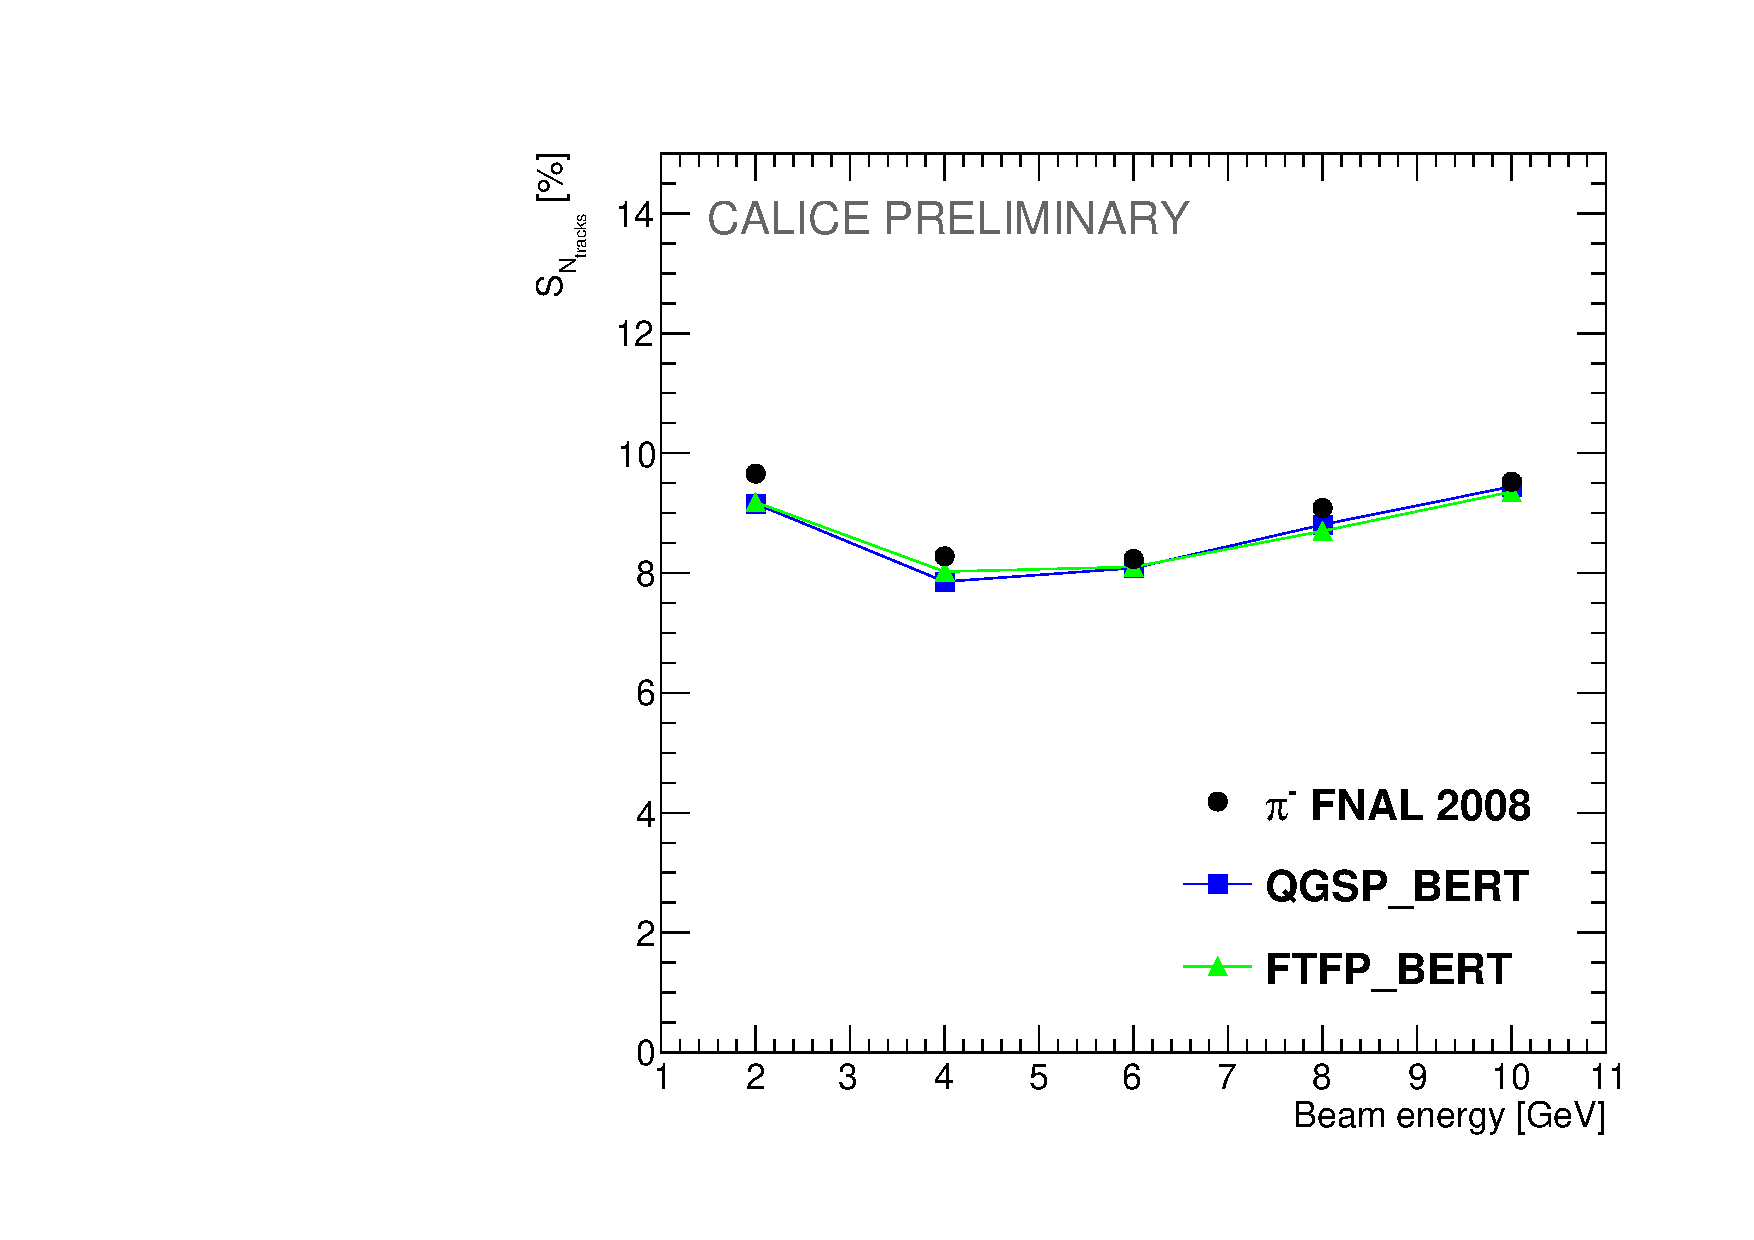
\includegraphics[width=.90\linewidth]{ECAL/plots/delta-ntracks-graph.pdf}
		\caption{\label{fig:dtracksgraph}}
	\end{subfigure}
	\caption{\label{fig:fulltrackgraph} \sl Mean number of secondary tracks $\left<N_{tracks}\right>$ for $\varepsilon = 0.03$ (a) and the corresponding sensitivity according to Eq.~\ref{eq:sens} of $\left<N_{tracks}\right>$ on the \ep\,(b) for data and Monte Carlo simulations for two {\sc Geant}4 physics lists as a function of the beam energy (from 2 to 10\,GeV). The sensitivity, see Eq.~\ref{eq:sens}, is estimated by the mean difference in $N_{tracks}$ for $\varepsilon_1 = 0.04$ and $\varepsilon_2 = 0.02$ normalised to the result for $\varepsilon_{nom} = 0.03$. Events without a detected interaction region according to Sec.~\ref{sec:iazone} are discarded. Error bars represent statistical errors and the error band the systematic error from the correction for double $\pi$ events.}
\end{figure}

%|||||||||||||||||||||Hit distribution||||||||||||||||||||||


\subsection{Number of hits per track}
The number of hits per track $N_{hits}^t$ is an essential feature to characterise the reconstructed tracks. 
The histograms of $N_{hits}^t$ for 2 and 10\,GeV beam energy are shown in Fig. \ref{fig:trackhitsexample}.
The distributions obtained for data and Monte Carlo agree in many bins within statistical errors and are therefore in good overall agreement with each other. 

Figure \ref{fig:trackshitsgraph} shows the dependence of $\left<N_{hits}^t\right>$ on the beam energy for data, \ftfp\ and \qgsp\ Monte Carlo simulations. The Monte Carlo models agree with the data within 5\%.  For energies greater than 4\,GeV both models are however systematically above  the data.
%The parametric uncertainty for the number of hits per track is defined as $\Delta N_{hits}^t = <N_{hits}^t(\varepsilon = 0.04) - N_{hits}^t(\varepsilon = 0.02)> /  <N_{hits}^t(\varepsilon = 0.03)>$. 
The sensitivity to the \ep\  as defined by Eq.~\ref{eq:sens} for ${\cal O}=N_{hits}$, $\varepsilon_{1},=0.04$, $\varepsilon_{2},=0.02$ and $\varepsilon_{nom.}=0.03$ is shown in Fig. \ref{fig:dtrackshitsgraph}. For the chosen parameter range the sensitivity increases with increasing beam energy from 1\% to about 5\% for both, data and the three {\sc Geant4} physics lists. 
%Figure \ref{fig:dtrackshitsgraph} demonstrates a similar behavior of parametric uncertainty on $N_{hits}^t$ for data and Monte Carlo. 

\begin{figure}
	\centering
	\begin{subfigure}{0.5\textwidth}
		\centering
		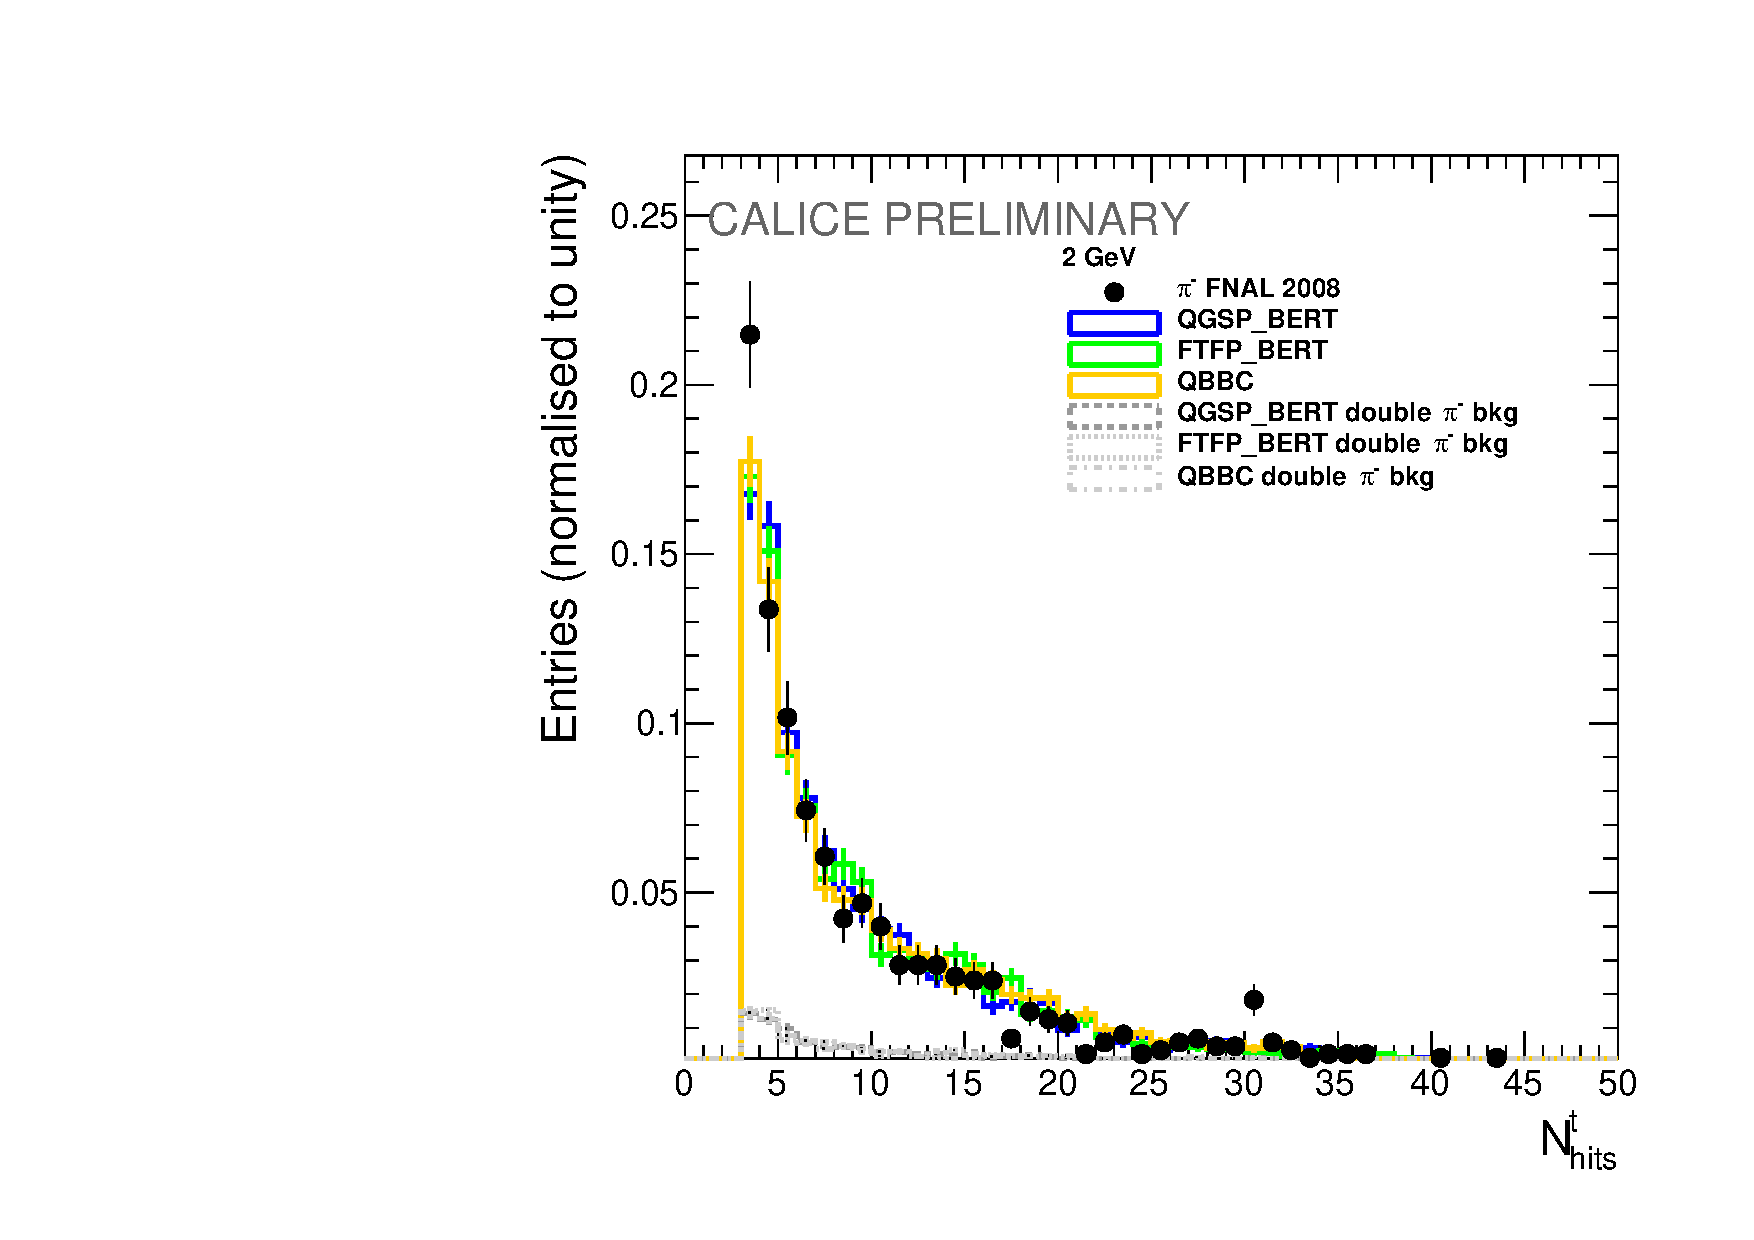
\includegraphics[width=.90\linewidth]{ECAL/plots/number-2.pdf}
		\caption{\label{fig:trh2} }
	\end{subfigure}% 
	\begin{subfigure}{0.5\textwidth}
		\centering
		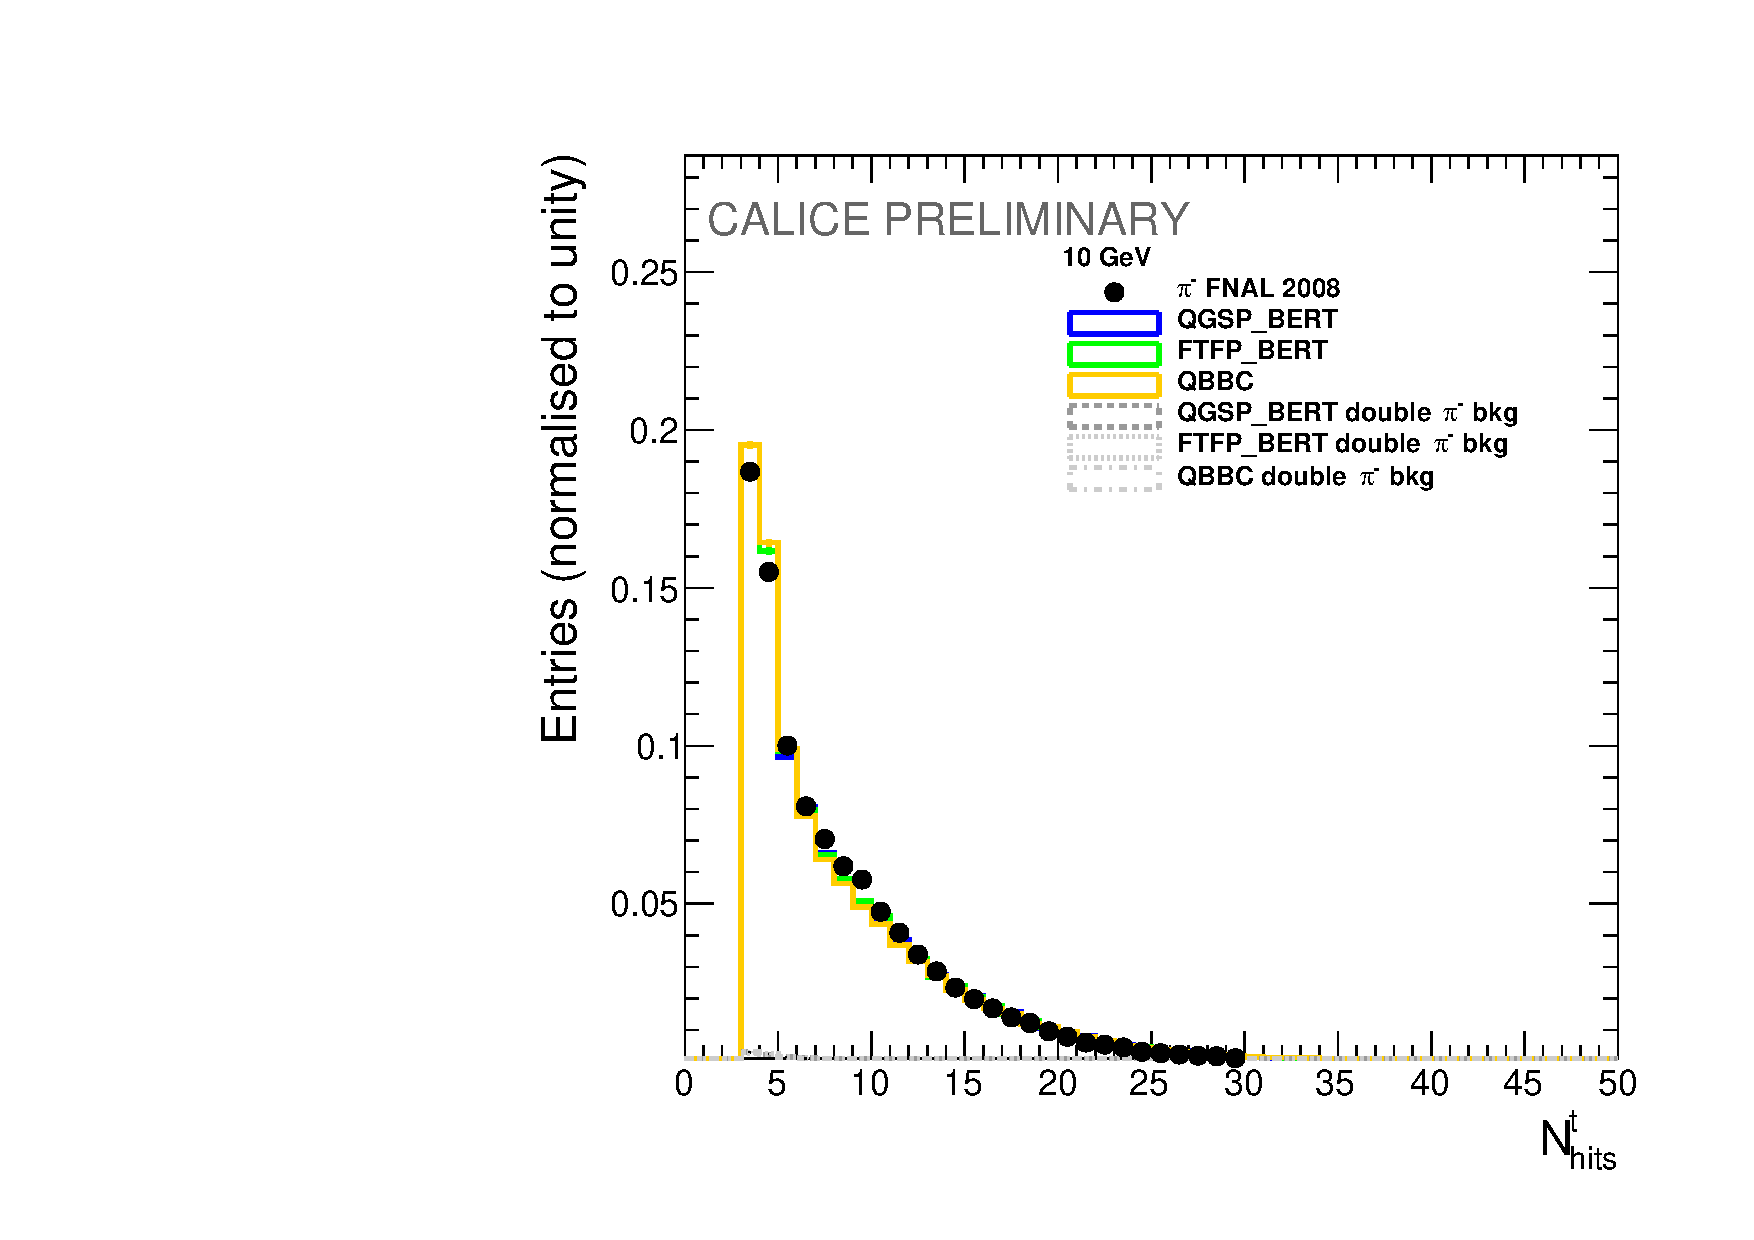
\includegraphics[width=.90\linewidth]{ECAL/plots/number-10.pdf}
		\caption{\label{fig:trh10} }
	\end{subfigure}
	\caption{\label{fig:trackhitsexample} \sl A comparison of the number of hits per reconstructed track between data and Monte Carlo simulations for two {\sc Geant}4 physics lists  or energies of the primary particle of 2 (a) and 10 (b) GeV, respectively. Events without a detected interaction region according to Sec.~\ref{sec:iazone} are discarded. The distributions are normalised to unity. Error bars represent statistical uncertainties only.}
\end{figure}

\begin{figure}
	\centering
	\begin{subfigure}{0.5\textwidth}
		\centering
		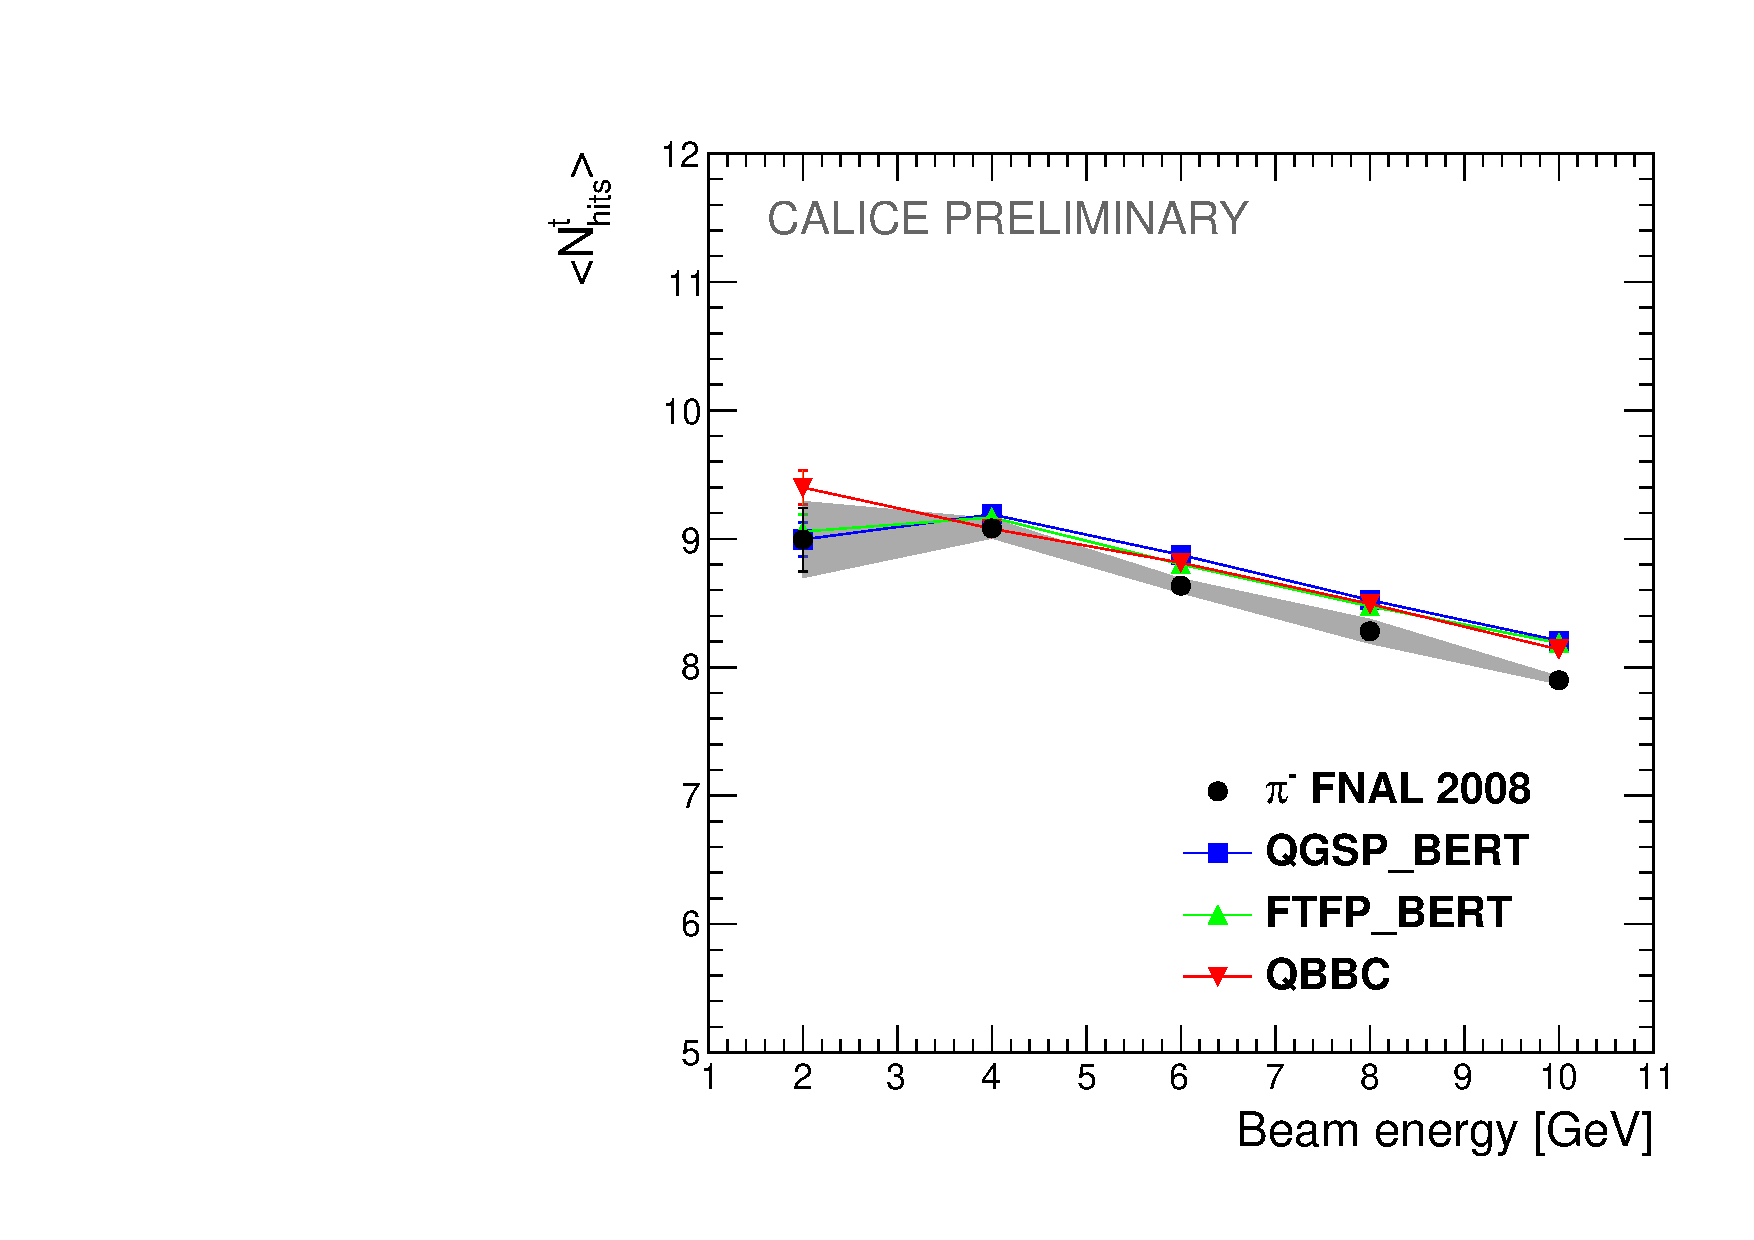
\includegraphics[width=.90\linewidth]{ECAL/plots/number-graph.pdf}
		\caption{\label{fig:trackshitsgraph}}
	\end{subfigure}% 
	\begin{subfigure}{0.5\textwidth}
		\centering
		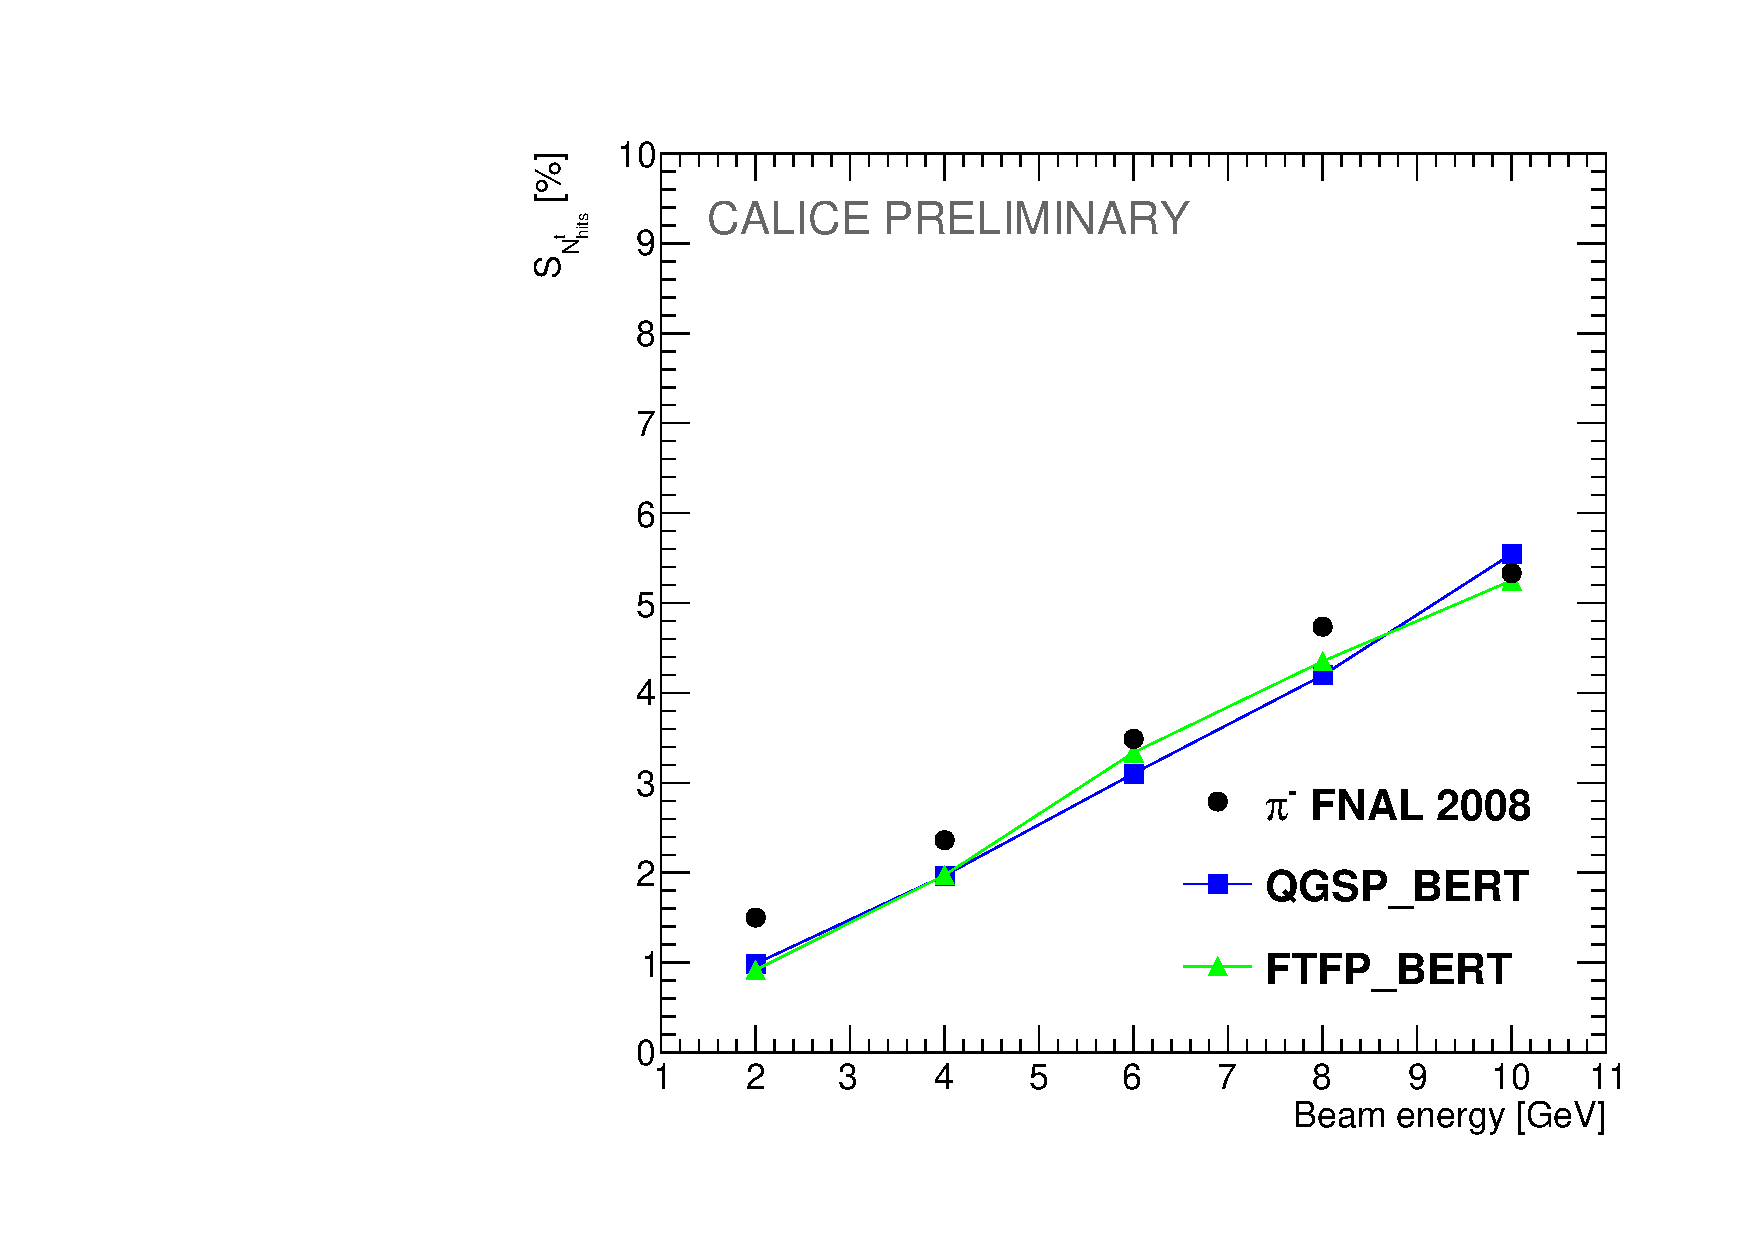
\includegraphics[width=.90\linewidth]{ECAL/plots/delta-number-graph.pdf}
		\caption{\label{fig:dtrackshitsgraph}}
	\end{subfigure}
	\caption{\label{fig:fulltrackhitsgraph} \sl Mean number of hits per reconstructed track  $\left<N_{hits}^t\right>$ for $\varepsilon = 0.03$  (a) and the corresponding sensitivity according to Eq.~\ref{eq:sens} of  $\left<N_{hits}^t\right>$ on the \ep\, (b) for data and Monte Carlo simulations for two {\sc Geant}4 physics lists as a function of beam energy (from 2 to 10\,GeV). Events without a detected interaction region according to Sec.~\ref{sec:iazone} are discarded. The sensitivity, see Eq.~\ref{eq:sens}, is estimated by the mean difference in $N_{hits}^t$ for $\varepsilon_1 = 0.04$ and $\varepsilon_2 = 0.02$ normalised to the result for $\varepsilon_{nom} = 0.03$. Error bars represent statistical errors and the error band the systematic error from the correction for double $\pi$ events.}
\end{figure}


%|||||||||||||||||||Angular distribution||||||||||||||||||||
\subsection{Angular distributions}
Due to the high granularity of the \ecal\, further tracking observables as the polar ($\theta$) and azimuthal ($\phi$) angles of secondary tracks become available.
Without a magnetic field, the secondary particles from hadronic interaction undergo only multiple elastic scattering in the detector material. Therefore, the direction of the initial momentum coincides approximately with the direction of the track that is visible in the \ecal.
Both angles are measured with respect to the $z$-axis in the right-handed coordinate frame defined in Sec.~\ref{sec:fnal}. The track direction is calculated from the position of the first and last hit of the track along the $z$-axis. 

Figures \ref{fig:thetaexample} and \ref{fig:phiexample} display histograms of the $\theta$ and $\phi$ angles, respectively, for 2 and 10\,GeV data and simulations based on the \ftfp\ an \qgsp\ physics lists. 

When corrected for the staggering of the detector layers in $x$-direction~\cite{Anduze:2008hq}, the pad coordinates of the \ecal\ define a grid with a step width of about 1\,cm in lateral direction. 
%The \tfa\ produces tracks with start and end points that are fixed to discrete calorimeter hit coordinates. 
This leads to a discretisation of the measured track direction and, therefore, to the $\phi$ and $\theta$ distributions in Figs. \ref{fig:thetaexample} and \ref{fig:phiexample}. In particular, $\phi$, angles that are a multiple of $\phi/4$ are privileged.
For 2 and 10\,GeV beam energy the {\sc Geant4} physics lists produce tracks with a similar angular distribution and reproduce the measured distributions adequately, which gives evidence that the \ecal\ geometry is correctly implemented into the Monte Carlo simulation.

The mean $\theta$ angle, $\left<\theta\right>$, that can be interpreted as a measure of the collimation of the secondary particles, as a function of the beam energy is shown in Fig. \ref{fig:thetagraph}. 
It can be seen that $\left<\theta\right>$ has only a weak dependence on the beam energy but shows the tendency to decrease as expected due to the increase of the boost transferred to the secondary particles.  The data are reproduced within a few \% by the Monte Carlo simulations. However, in case of the \qgsp\ physics list the collimation features a step between energies of the primary particle of 8\,GeV and 10\,GeV, i.e. at the transition between Bertini and LEP cascades. It seems also that the curve for \ftfp\ physics flattens out above 4\,GeV beam energy, corresponding to the transition between Bertini and Fritiof models.
%cross section of hadronic interaction
%Secondary tracks, produced by the two Monte Carlo physics lists have on average 10\%  smaller polar angles than those in in data for all beam energies. This plot reveals some internal properties of the given physics lists: 
%\begin{itemize}
%\item The \qgsp\ physics list produces tracks with smaller $<\theta>$ for 10\,GeV initial $\pi^-$ than for 8\,GeV, which corresponds to the transition between Bertini and LEP cascades.
%\item The \ftfp\ physics list changes tendency above 4\,GeV beam energy, corresponding to the transition between Bertini and Fritiof models.
%\item The values of $<\theta>$ are exactly the same for 2 and 4\,GeV initial particle energies for both physics lists, where the same model is used.
%\end{itemize}

The sensitivity to the \ep\  as defined by Eq.~\ref{eq:sens} for ${\cal O}=\theta$, $\varepsilon_{1},=0.04$, $\varepsilon_{2},=0.02$ and $\varepsilon_{nom.}=0.03$ is shown in Fig. \ref{fig:dthetagraph}. In both cases the sensitivity is between 1.5\% and 3\%.

%As a measure for the parametric uncertainty, introduced by the $\varepsilon$ parameter, the estimator $\Delta \theta = <\theta(\varepsilon = 0.04) - \theta(\varepsilon = 0.02)> /<\theta(\varepsilon = 0.03)> $ is used.
%This parametric uncertainty, shown in Fig. \ref{fig:dthetagraph} is comparable for data and Monte Carlo. 

%As supplementary information Fig. \ref{fig:thetaepsilonsys} shows a study of the dependence of $<\theta>$ on $\varepsilon$ for the different beam energies. The dependence is moderate except for 2\,GeV. In all
%cases the results for $\varepsilon = 0.03$ are approximately in the center of a broad minimum corroborating the stability of the results shown in Figs. \ref{fig:thetaexample} and \ref{fig:phiexample}. 

\begin{figure}
	\centering
	\begin{subfigure}{0.5\textwidth}
		\centering
		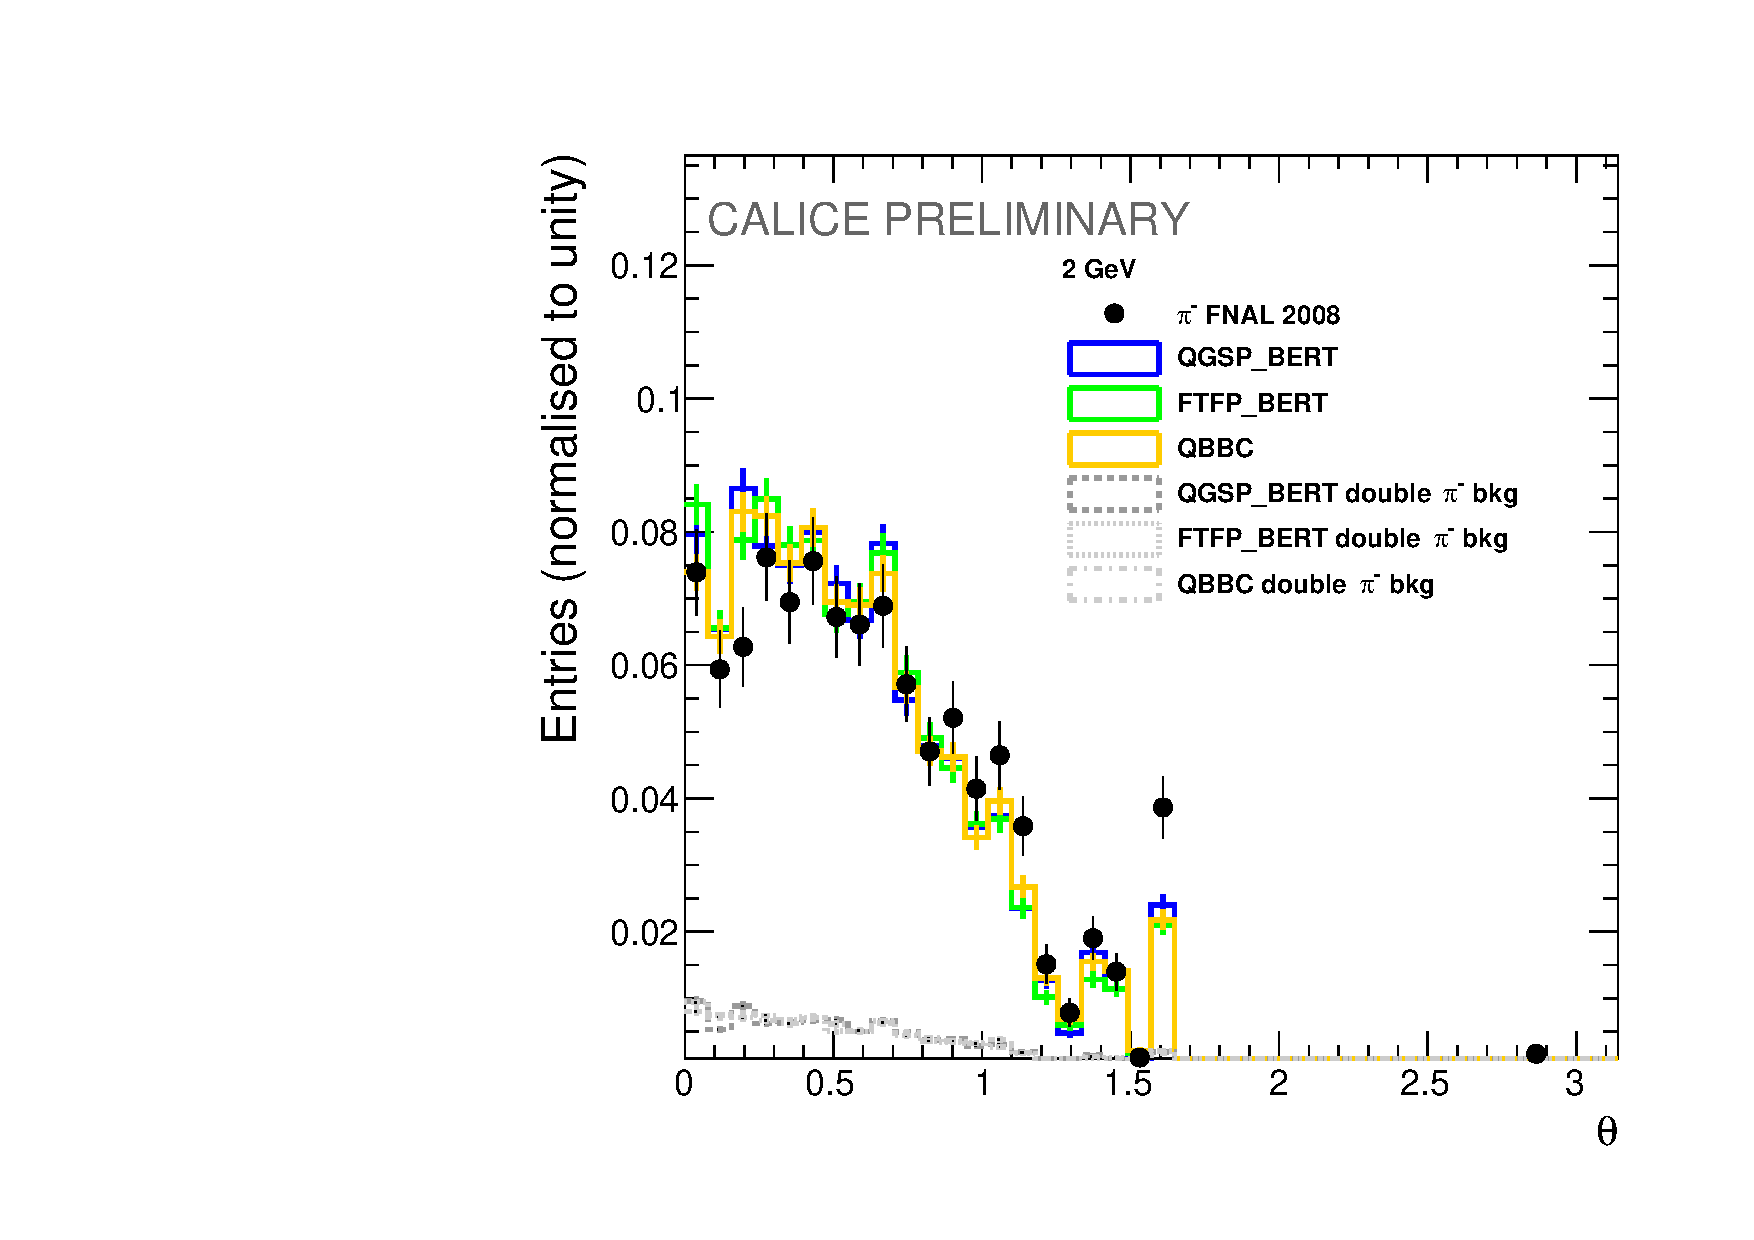
\includegraphics[width=.90\linewidth]{ECAL/plots/theta-2.pdf}
		\caption{\label{fig:theta2} }
	\end{subfigure}% 
	\begin{subfigure}{0.5\textwidth}
		\centering
		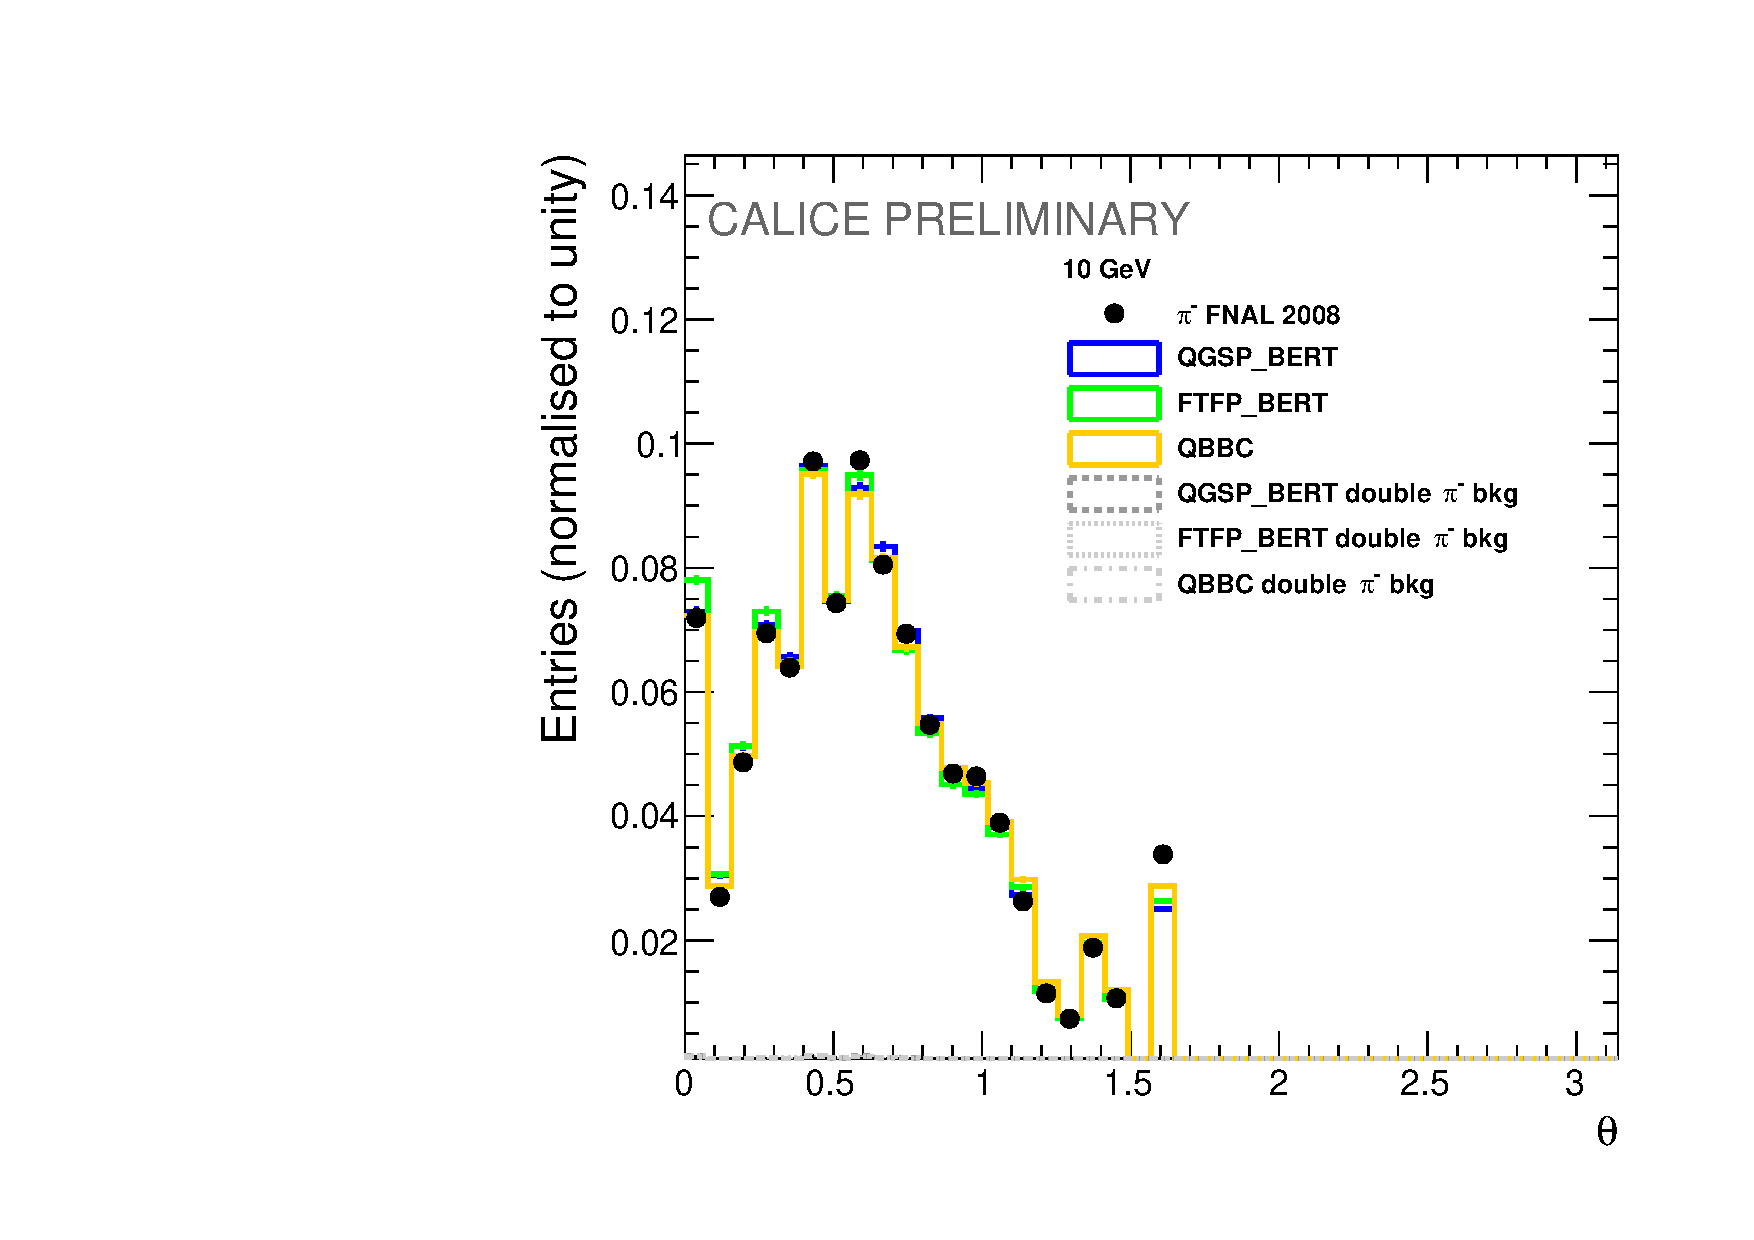
\includegraphics[width=.90\linewidth]{ECAL/plots/theta-10.pdf}
		\caption{\label{fig:theta10} }
	\end{subfigure}
	\caption{\label{fig:thetaexample} \sl Comparison of the polar angle $\theta$ of secondary tracks found between data and Monte Carlo simulations for two {\sc Geant}4 physics lists for energies of the primary particle of 2 (a) and 10 (b) GeV, respectively. Events without a detected interaction region according to Sec.~\ref{sec:iazone} are discarded. Error bars represent statistical uncertainties only.}
\end{figure}

\begin{figure}
	\centering
	\begin{subfigure}{0.5\textwidth}
		\centering
		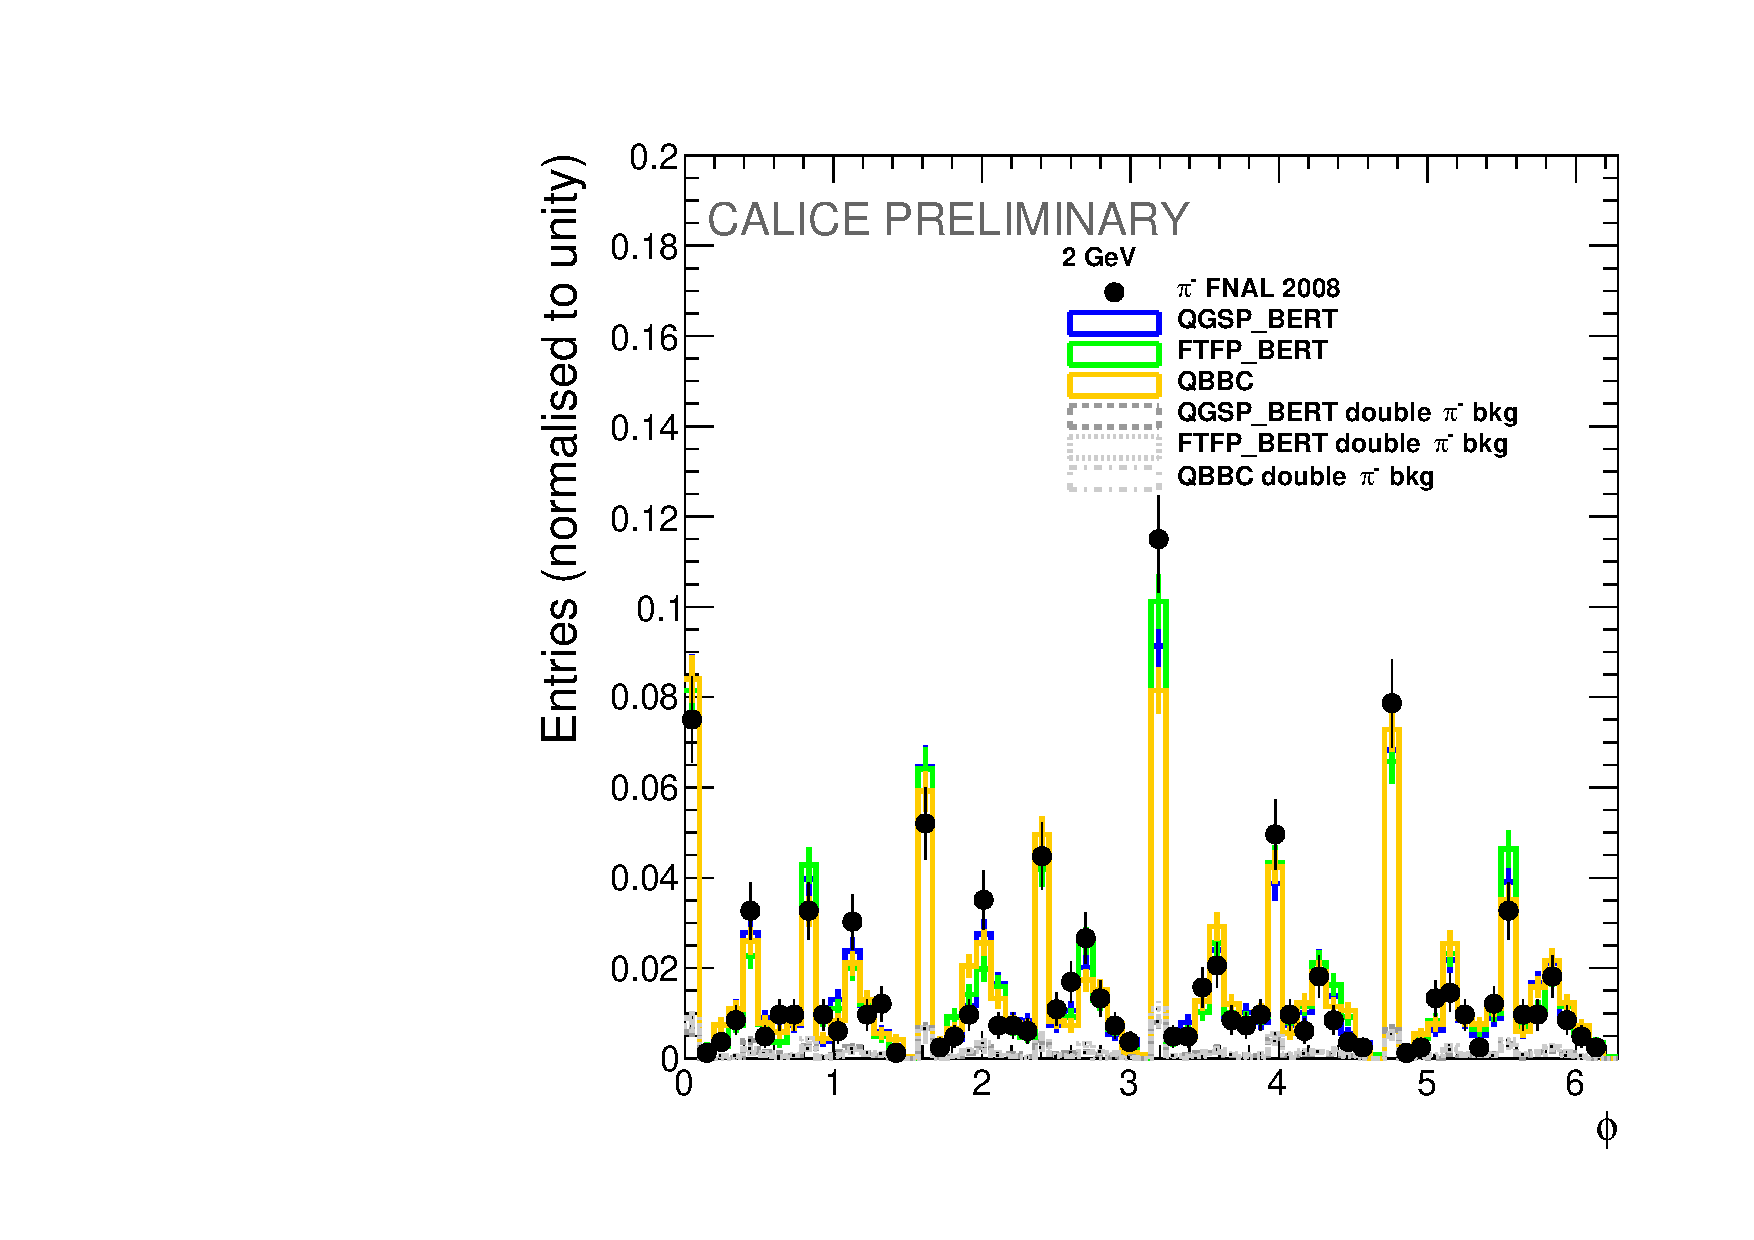
\includegraphics[width=.90\linewidth]{ECAL/plots/phi-2.pdf}
		\caption{\label{fig:phi2} }
	\end{subfigure}% 
	\begin{subfigure}{0.5\textwidth}
		\centering
		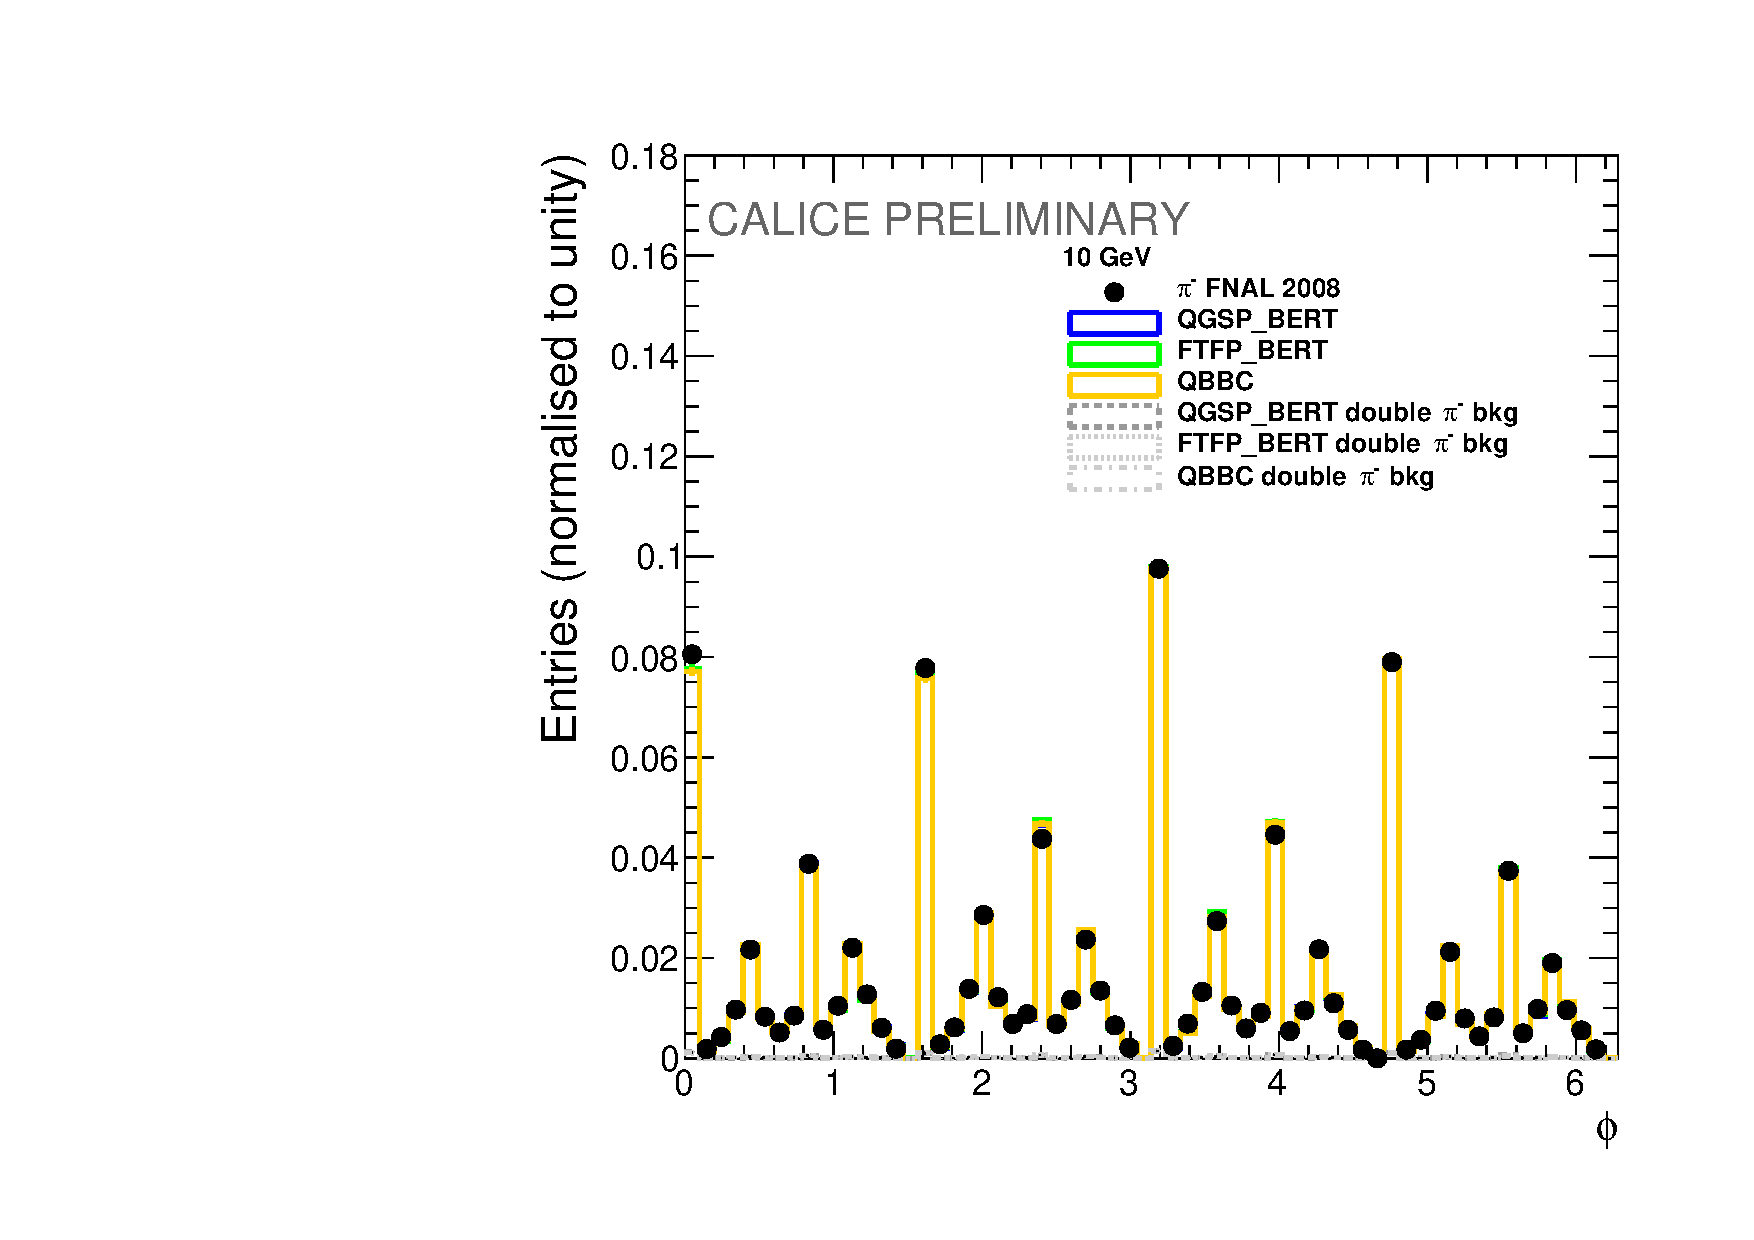
\includegraphics[width=.90\linewidth]{ECAL/plots/phi-10.pdf}
		\caption{\label{fig:phi10} }
	\end{subfigure}
	\caption{\label{fig:phiexample} \sl Comparison of the azimuthal angle $\phi$ of secondary tracks between data and Monte Carlo simulations for two {\sc Geant}4 physics lists for 2 (a) and 10 (b) GeV beam energies. Events without a detected interaction region according to Sec.~\ref{sec:iazone} are discarded. Error bars represent statistical uncertainties only.}
\end{figure}

\begin{figure}
	\centering
	\begin{subfigure}{0.5\textwidth}
		\centering
		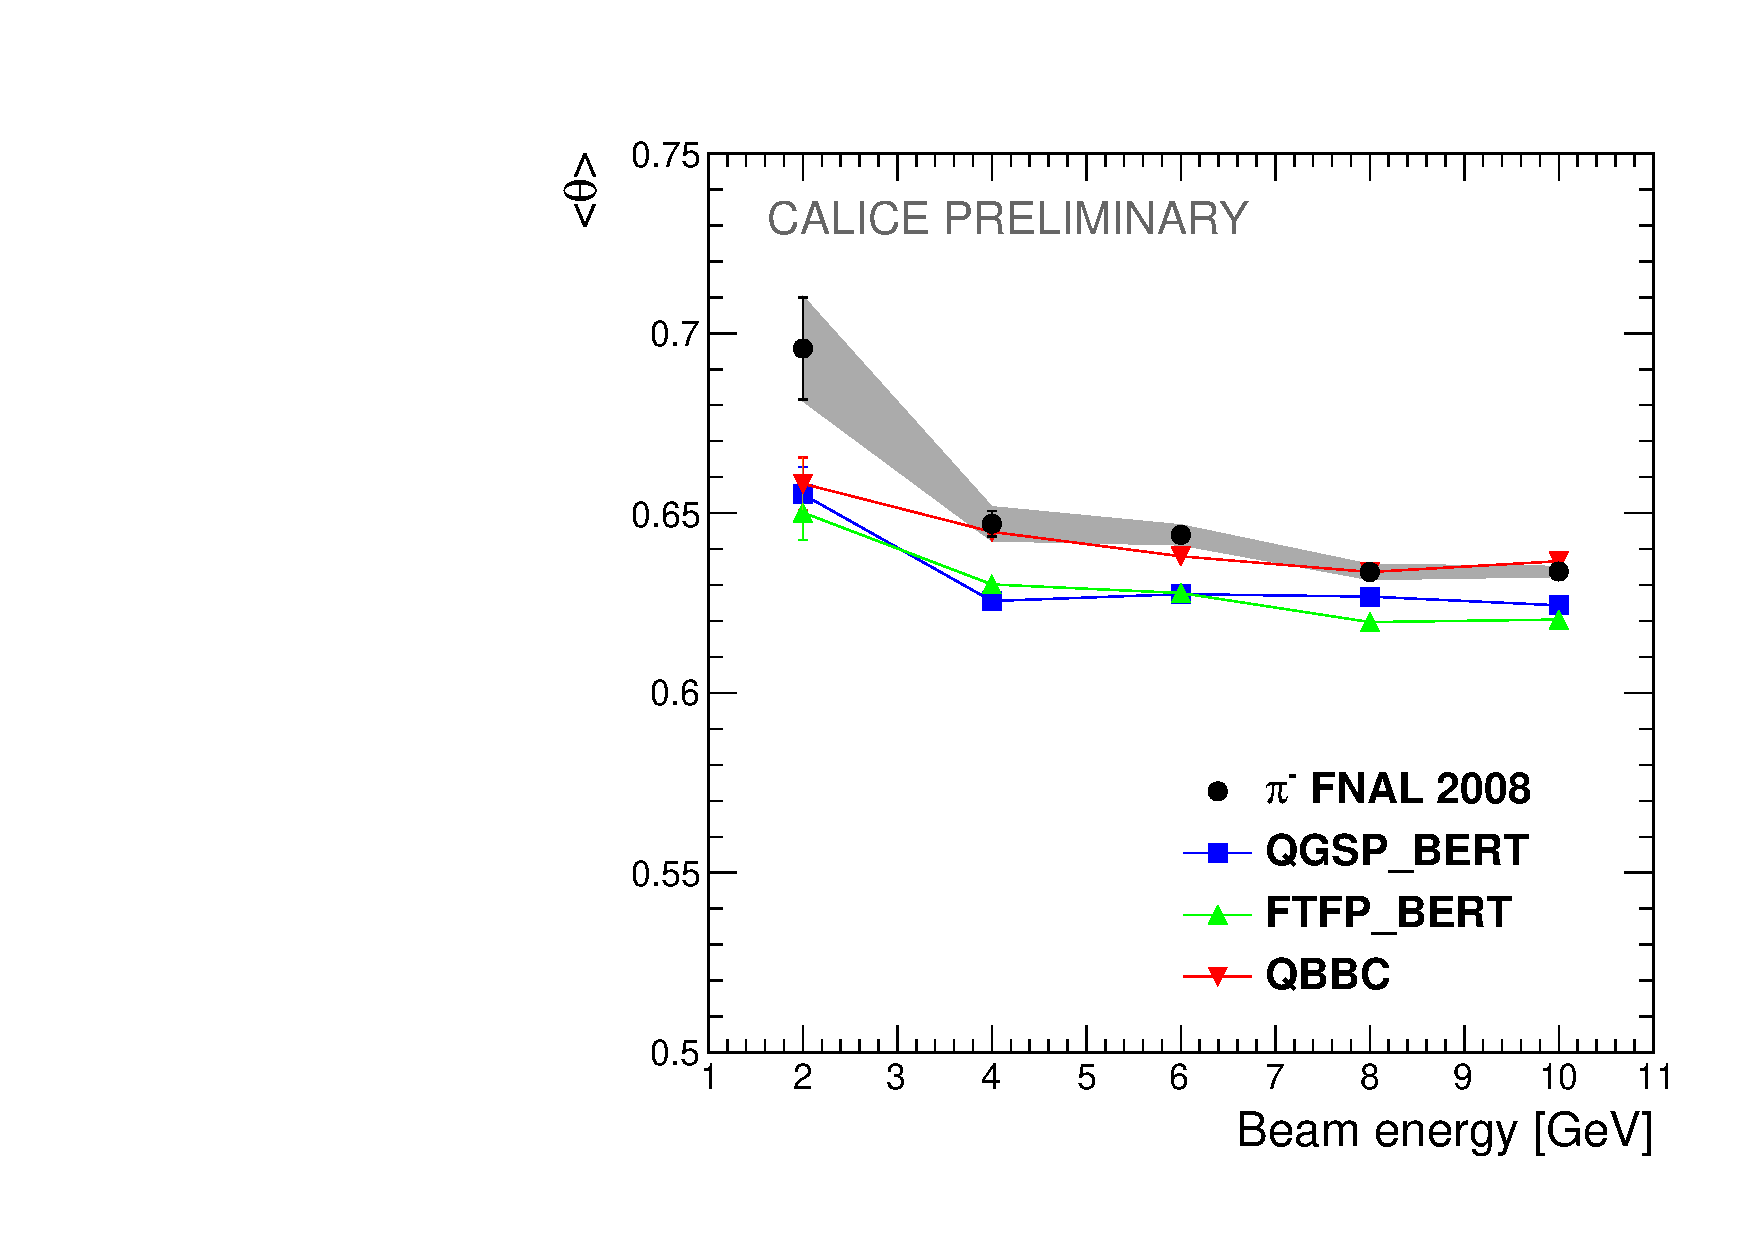
\includegraphics[width=.90\linewidth]{ECAL/plots/theta-graph.pdf}
		\caption{\label{fig:thetagraph}}
	\end{subfigure}% 
	\begin{subfigure}{0.5\textwidth}
		\centering
		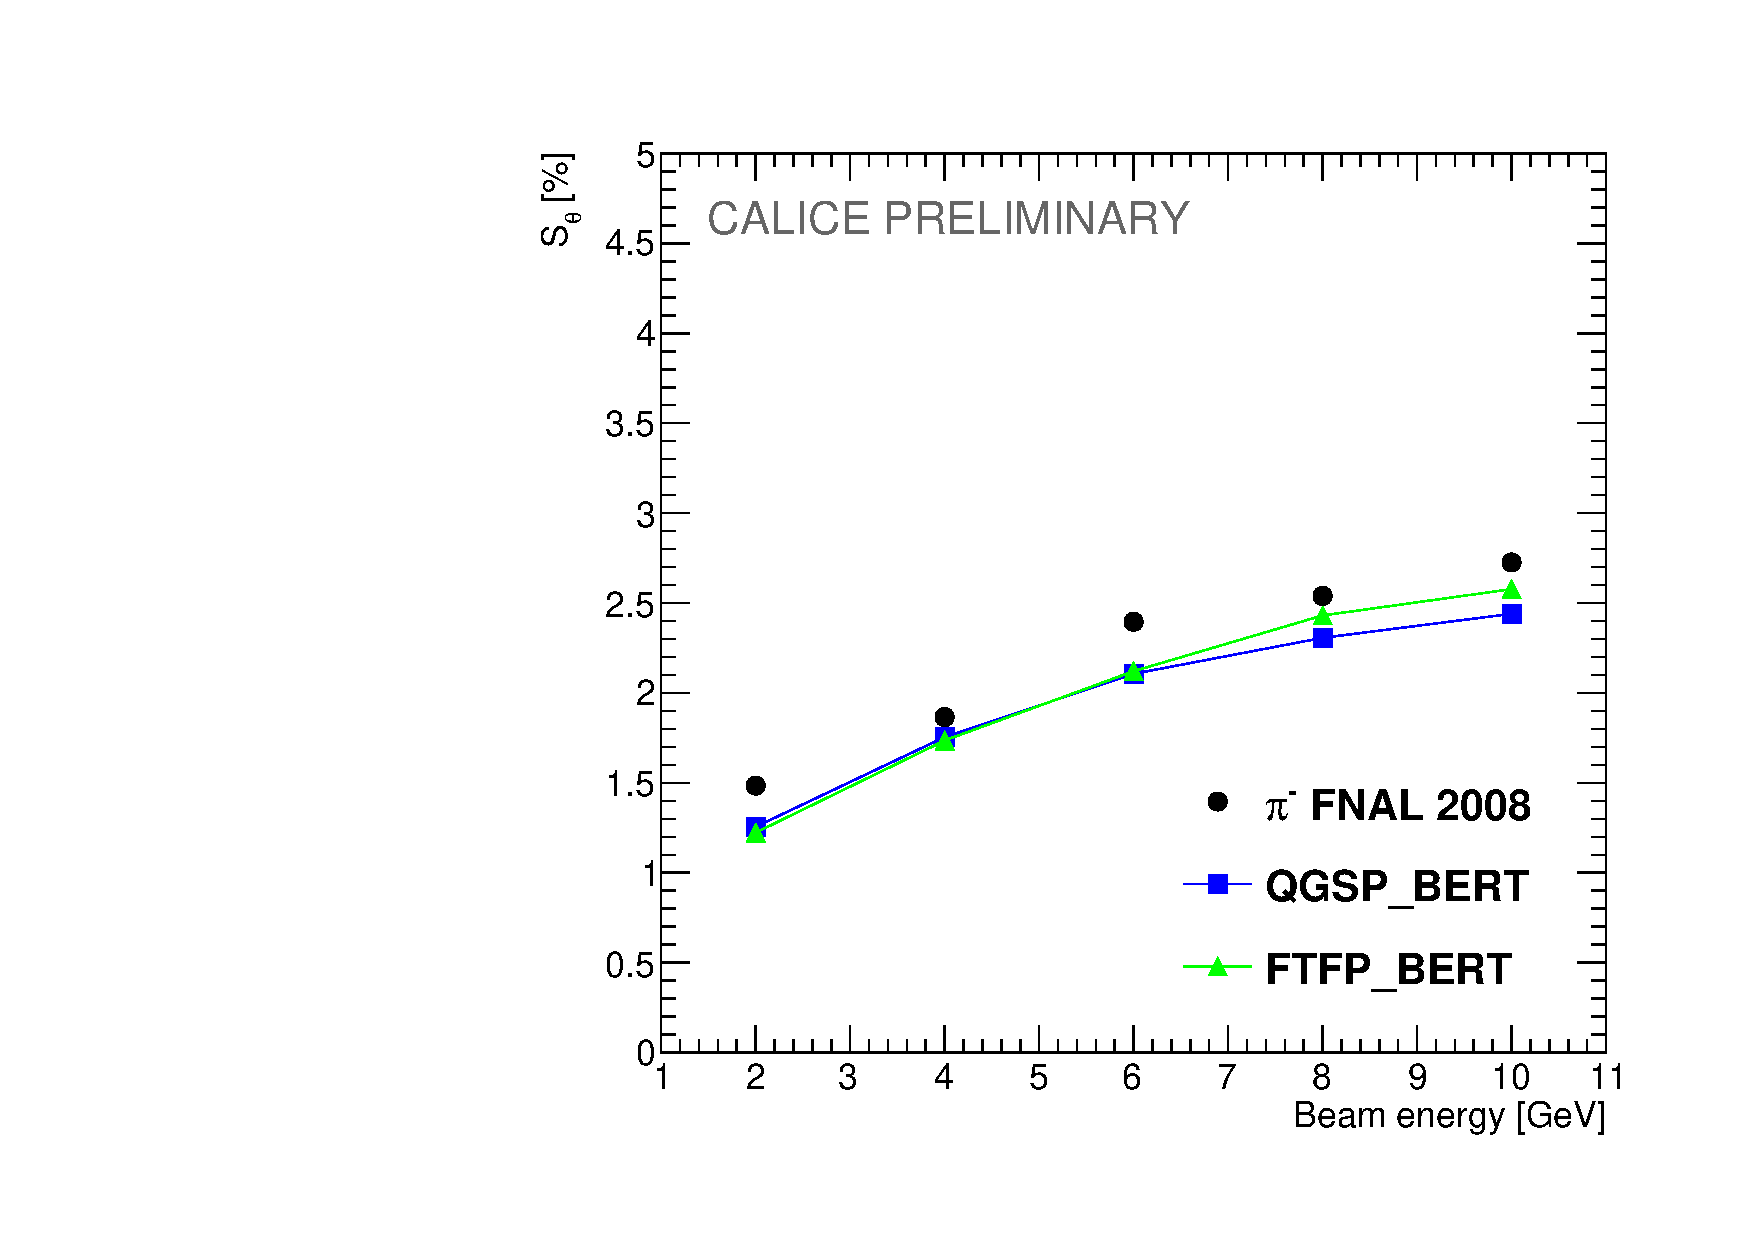
\includegraphics[width=.90\linewidth]{ECAL/plots/delta-theta-graph.pdf}
		\caption{\label{fig:dthetagraph} }
	\end{subfigure}
	\caption{\label{fig:fullthetagraph} \sl Mean polar angle $\left<\theta\right>$ of secondary tracks for $\varepsilon = 0.03$  (a) and the corresponding sensitivity according to Eq.~\ref{eq:sens} of $\left<\theta\right>$ on the \ep\,(b) for data and Monte Carlo simulations for two {\sc Geant}4 physics lists as a function of beam energy. The sensitivity, see Eq.~\ref{eq:sens}, is estimated by the mean difference in $\theta$ for $\varepsilon = 0.04$ and $\varepsilon_{nom} = 0.02$. Events without a detected interaction region according to Sec.~\ref{sec:iazone} are discarded. Error bars represent statistical errors and the error band the systematic error from the correction for double $\pi$ events.}
\end{figure}
A further discussion on the relationship between the \ep ,  the polar angle $\theta$ and the track length $l$ can be found in Appendix~\ref{app:b}.

%||||||||||||||||||||MPV energy deposition|||||||||||||||||||||
\subsection{Energy deposition by secondary tracks}

%The developed \tfa\ can select tracks from MIP-like particles in the \ecal\ that have no electron contamination.
%The secondary tracks in hadronic cascades should have the same mean energy deposition for any initial particle energy.
At energies relevant for this study, the secondaries that create sizeable tracks, cross the detector volume as minimal ionising particles. 
%This motivates to investigate whether the secondary tracks can be used for an in-situ MIP calibration of the \ecal. 
This fact may be exploited for an in-situ calibration of the detector or at least for a monitoring of the response of individual detector regions. For this purpose the following additional selection cuts are applied: 
\begin{itemize}
	\item The events are required to have more than one track and an interaction region to suppress soft inelastic scattering interaction for lower energies;
	\item The reconstructed tracks should have a length $l\geq 8$ and $l / N_{hits} > 0.9$ to select long pencil-like tracks;
	\item the reconstructed tracks should have an polar angle $\theta < 0.3$ to reduce the angular dependence of the energy depositions.
\end{itemize}

The energy deposition by secondary tracks $E_{dep}^t$ using data for 2 and 10\,GeV beam energy is displayed in Fig. \ref{fig:calib}. Both distributions peak at around 1\,MIP as expected for straight MIP like tracks. Overlaid is a fit of the convolution of a Landau and a Gaussian that approximates well the measured distribution. However, as can be already inferred from Fig.~\ref{fig:calib2}, the tighter selection criteria reduce considerably the statistics at 2\,GeV. As a consequence, the uncertainty on the fit is large for the 2\,GeV sample. The data at 2\,GeV are thus discarded in the following.

Figure \ref{fig:calibrationgraph} presents the dependence of the most probable value (MPV) of the energy deposition in secondary tracks on beam energy. 
It can be seen that the detector response is uniform within 1-2\% over the energy range of the primary particles in data and that also the energy deposition by the tracks is reproduced by the Monte Carlo simulations within 1-2\%.  

\begin{figure}
	\centering
	\begin{subfigure}{0.5\textwidth}
		\centering
		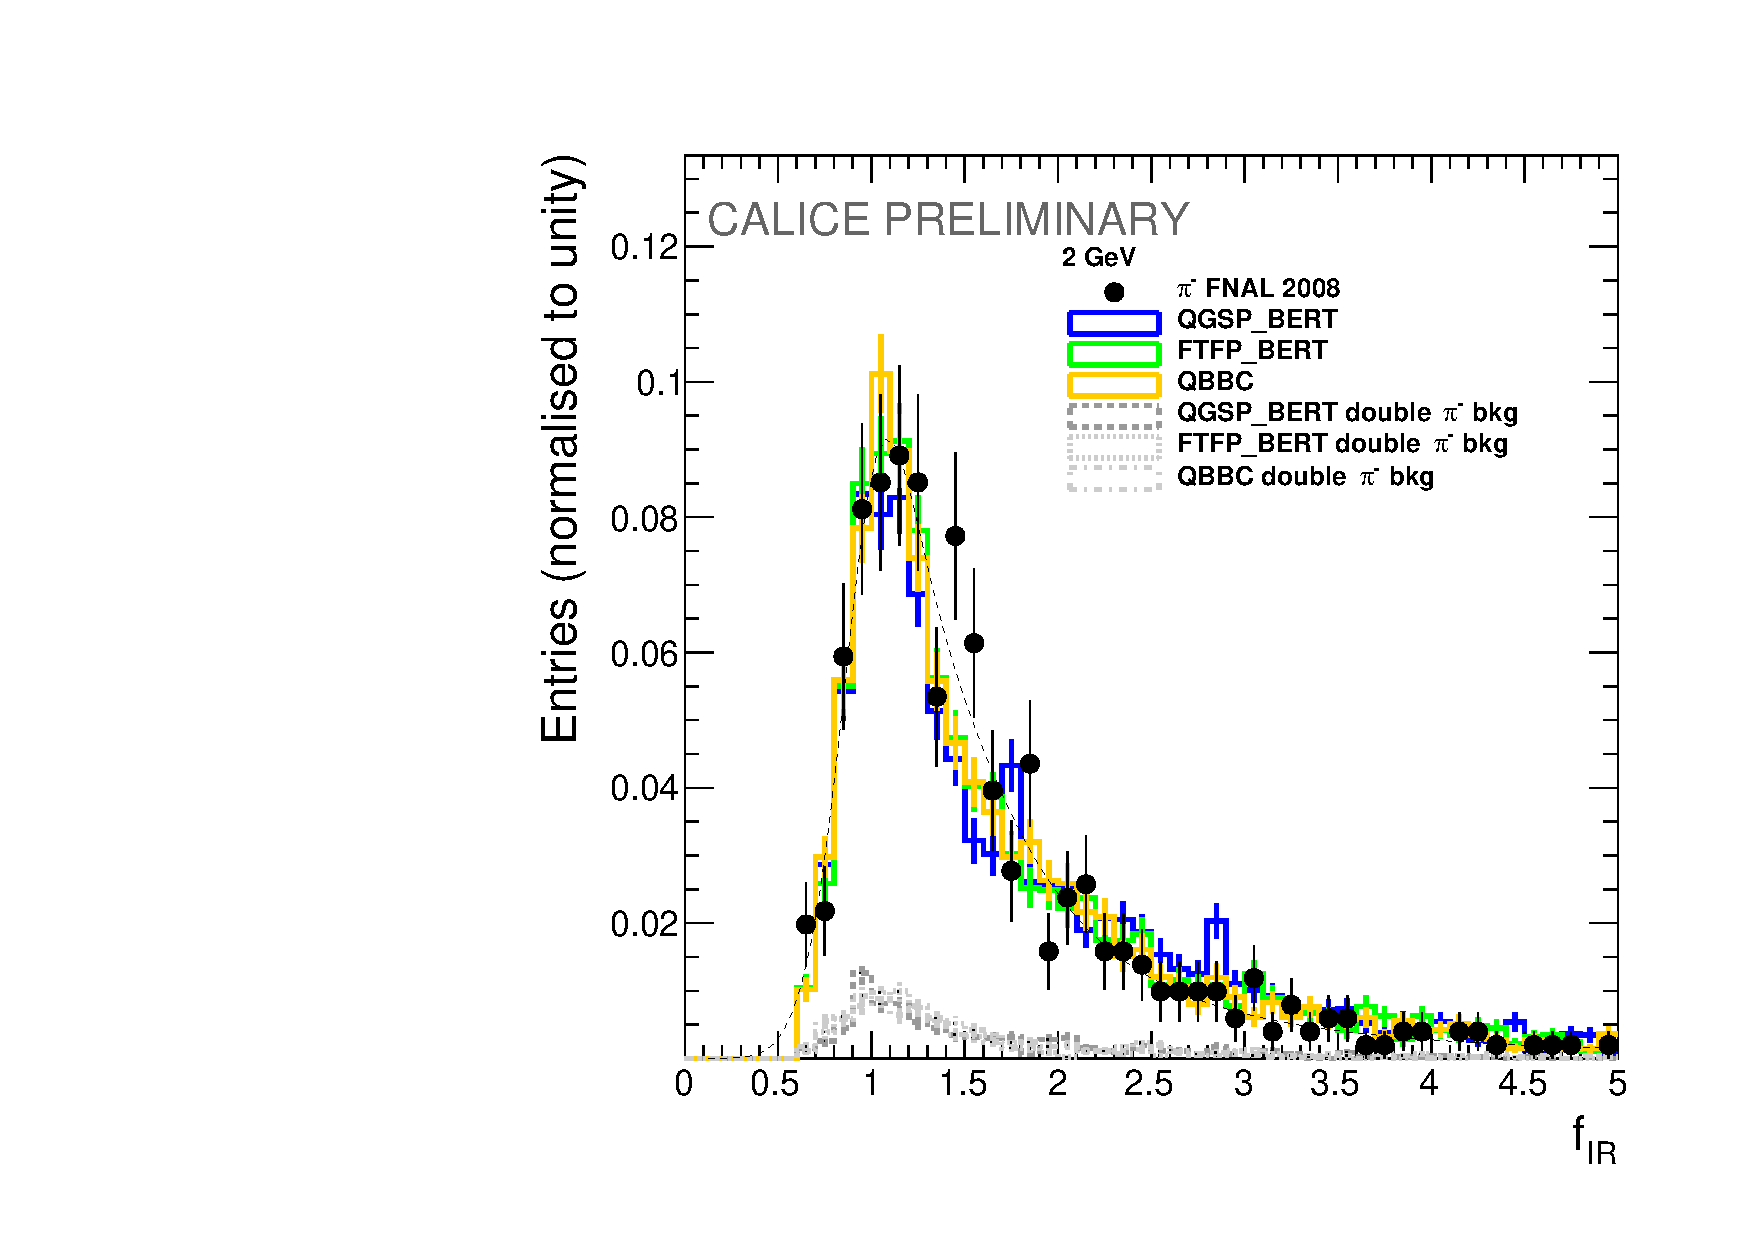
\includegraphics[width=.90\linewidth]{ECAL/plots/calibrationfit-2.pdf}
		\caption{\label{fig:calib2} }
	\end{subfigure}% 
	\begin{subfigure}{0.5\textwidth}
		\centering
		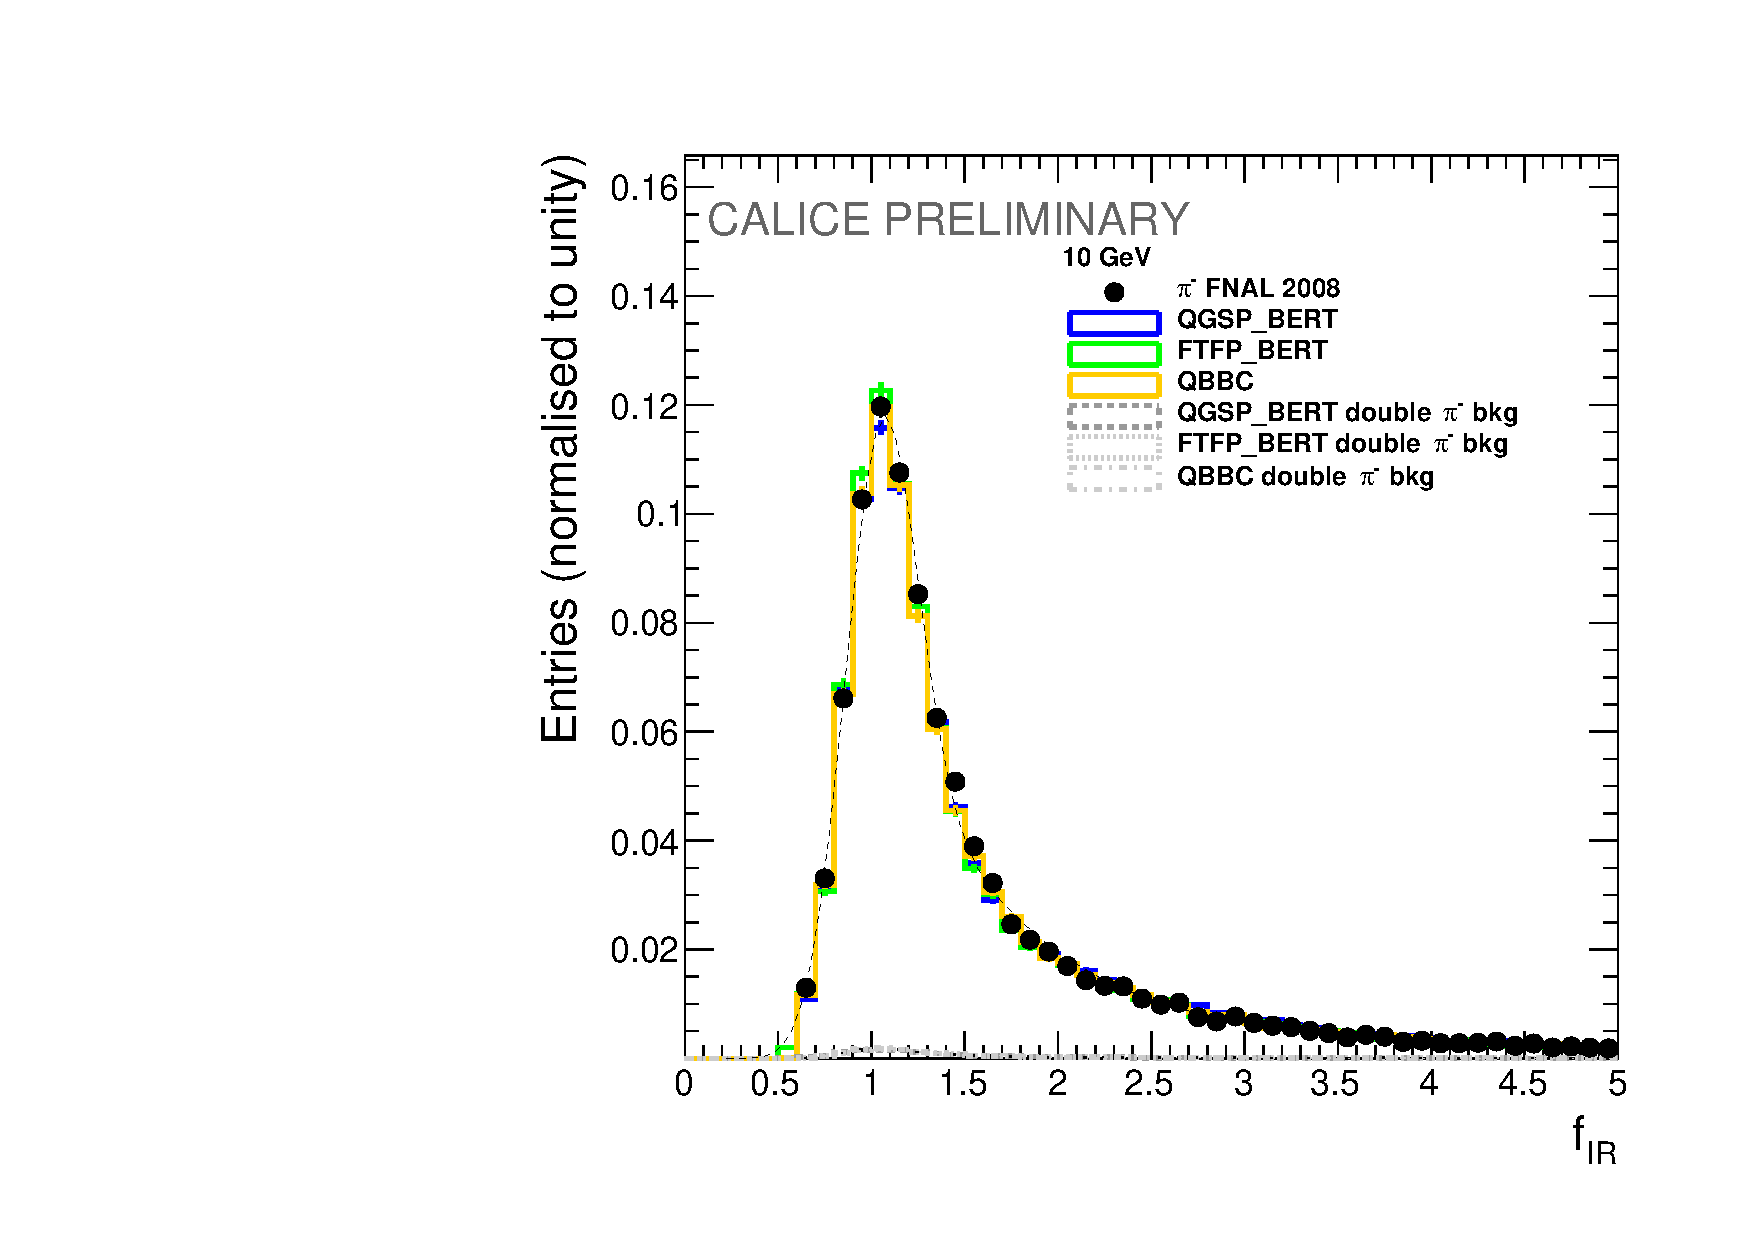
\includegraphics[width=.90\linewidth]{ECAL/plots/calibrationfit-10.pdf}
		\caption{\label{fig:calib10} }
	\end{subfigure}
	\caption{\label{fig:calib} \sl Histograms of the energy deposition in secondary tracks for the data with 2 (a) and 10 (b) GeV beam energies. The spectra are fitted by the convolution of a Landau and a Gaussian. Events without a detected interaction region according to Sec.~\ref{sec:iazone} are discarded. Error bars represent statistical uncertainties only.}
\end{figure}

\begin{figure}
	\centering
	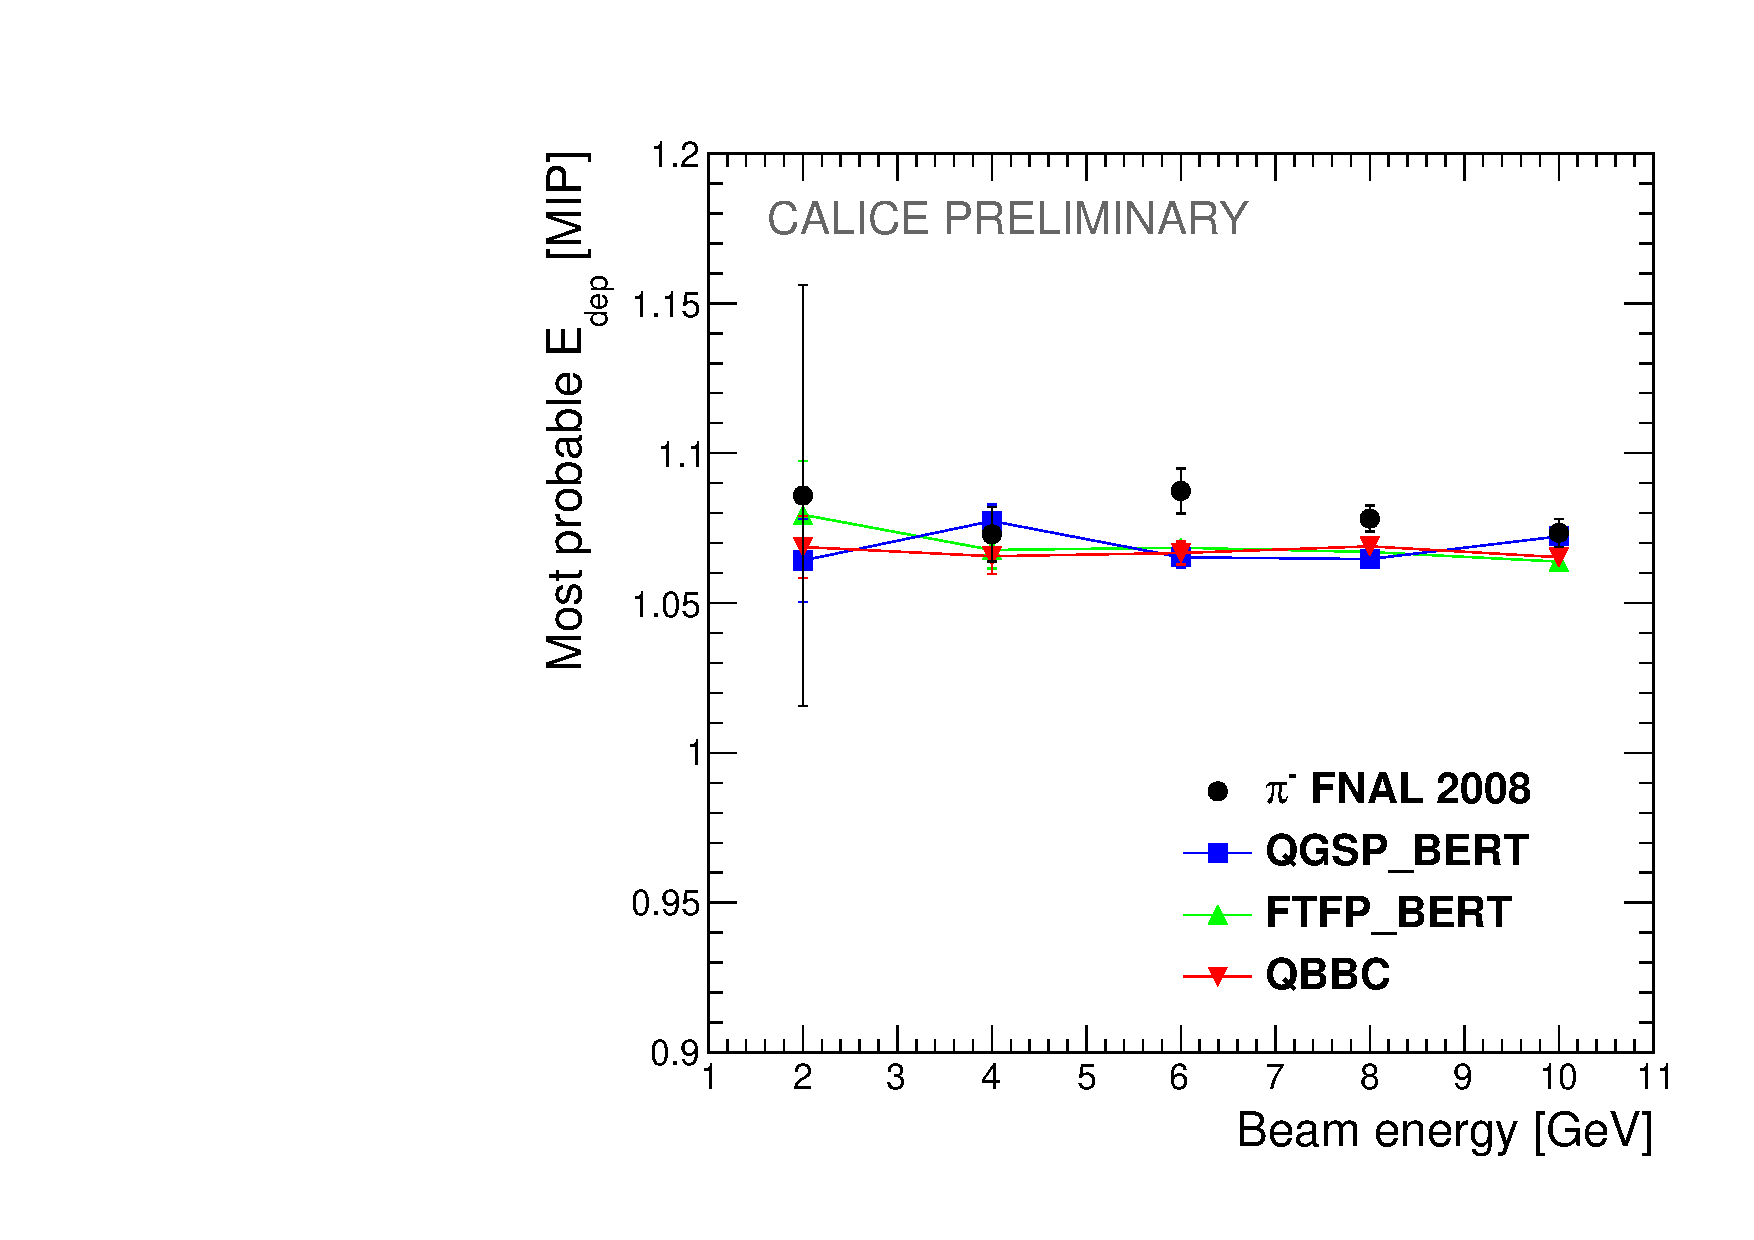
\includegraphics[width=0.5\textwidth]{ECAL/plots/calibrationfit-graph.pdf}
	\caption{\label{fig:calibrationgraph} \sl MPV of the Landau fit to the $E_{dep}^t$ distributions of the pencil-like secondary tracks as a function of the beam energy for $\pi^-$ data and three Monte Carlo samples. The MPV point the of 2\,GeV data sample is excluded because of the small statistics left after selection. Events without a detected interaction region  according to Sec.~\ref{sec:iazone} are discarded.  Error bars represent the statistical fit uncertainty.}
\end{figure}

This result is not trivial. It shows that the algorithm has indeed selected MIP-like secondary tracks since the MIP scale is expected to be independent of the underlying physics lists and the detector response should be largely independent of the energy of the primary particle. 

%-------------------------------------------------------------
%------------------------SUMMARY------------------------------
%-------------------------------------------------------------
\section{Summary and outlook}

This study reveals the outstanding potential of the CALICE \ecalp\ to obtain a detailed picture of the interactions of hadrons with matter. 
This note describes basic ideas and the application of a new simple \tfa\ for the \ecal. This algorithm allows for the reconstruction of tracks produced by secondary particles created in the interaction of hadrons with the absorber material, and hence to study the interaction region of hadronic showers in the \ecal. The \tfa\ produces a new set of differential observables, based on reconstructed tracks of secondary particles and the interaction region of the hadronic cascades. The results are stable w.r.t. small variations of the main parameter of the \tfa.

Data recorded in test beams at FNAL in 2008 with pions as primary particles with energies between 2 and 10\,GeV are compared with predictions by the physics lists \qgsp\, \ftfp\ and \qbbc as contained in {\sc Geant4} version 10.01. The accuracy with which the simulation describes the data varies with the beam energy and the chosen physics observable. In most of the cases data and Monte Carlo agree within 10\% without revealing a clear preference for one of the chosen physics lists. In this context it is worthwhile to remind that the interaction region is systematically 10\% wider than it is the case for the Monte Carlo simulation.

The largest source of discrepancy between data and Monte Carlo is the energy and radius of the interaction region. The measured energy deposition in the interaction region is up to 20\% higher than predicted by the Monte Carlo simulation.
The distributions of the number of secondary tracks and the number of hits per track for data are well described by the used physics lists. The polar angles of reconstructed tracks in the Monte Carlo simulation agree with data within 8\% on average and the distribution azimuthal angles is well reproduced by the Monte Carlo simulations even in view of the non trivial detector geometry.

%The new observables are sensitive to the different hadronic models implemented in the physics lists. 
%The mean polar angle of detected tracks as a function of the beam energy has a visible transition between Fritiof and Bertini cascades in the \ftfp\ physics list, as well as between Bertini and LEP models in the \qgsp\ physics list. The same effects can be seen for other observables. 

With respect to a more general outlook future work should aim at transferring the insights about the interaction region and the secondaries emerging from it to the optimisation of Particle Flow Algorithms.

A tighter track selection leads to clean MIP-like tracks. The detector response is stable to about 1-2\% over the tested energy range with an expected good agreement with Monte Carlo simulations. This observation can be exploited in the future as a starting point for a study on the possibility of an in-situ calibration or at least a regular monitoring of the detector by means of the selected tracks.  


%In conclusion, there is no preference for {\sc Geant4} physics lists as none of the two models, used in the analysis, describe the data in high detail. 
%-------------------------------------------------------------------
%-------------------------BIBLIOGRAPHY------------------------------
%-------------------------------------------------------------------
%\begin{thebibliography}{100} 
%\bibitem{bib:Calorimetry} J. C. Brient, H. Videau,\emph{ The calorimetry at the future $e^+e^-$ linear collider}, in: Proceedings of the APS / DPF / DPB Summer Study on the Future of Particle Physics (Snowmass 2001), 2001,arXiv:hep-ex/0202004v1.
%\bibitem{bib:ecal} The CALICE collaboration, \emph{Design and electronics commissioning of the physics prototype of a Si-W electromagnetic calorimeter for the International Linear Collider}, J. Instrum. 3 (2008) P08001, arXiv:0805.4833v1 [physics.ins-det]
%\bibitem{bib:Naomi} The CALICE Collaboration,  \emph{Testing Hadronic Interaction Models using a Highly Granular Silicon-Tungsten Calorimeter}, Nucl. Instrum. Meth. A Volume 794, Pages 240–254, arXiv:1411.7215v2 [physics.ins-det]
%\bibitem{bib:2010_CALICE_2} The CALICE Collaboration, C. Adloff, et al., \emph{Construction and Commissioning  of the CALICE Analog Hadron Calorimeter Prototype}, J. Instrum.~(5)  (2010) P05004, arXiv:1003.2662v1 [physics.ins-det].
%\bibitem{bib:2012_CALICE} The CALICE Collaboration, C. Adloff, et al., \emph{Construction and performance of a silicon photomultiplier/extruded scintillator tail-catcher and muon-tracker}, J. Instrum. (7) (2012) P04015, arXiv:1201.1653 [physics.ins-det].
%\bibitem{bib:G4pl} The {\sc Geant}4 Collaboration, \emph{Reference Physics Lists}, \url{http://Geant4.cern.ch/support/proc_mod_catalog/physics\_lists/referencePL.shtml}
%\bibitem{bib:HLi} \emph{Higgs Recoil Mass and Cross-Section Analysis at ILC And Calibration of the CALICE SiW ECAL Prototype}, Ph.D. thesis, Universit\'e Paris Sud   - Paris XI (2012).
%\bibitem{bib:2012_Doublet} P.Doublet, \emph{Hadrons dans un calorim\`etre \'electromagn\'etique   silicium-tungst\`ene hautement granulaire -- Production du quark top \'a   l'International Linear Collider}, Ph.D. thesis, Universit\'e Paris Sud   - Paris XI (2012).
%\end{thebibliography}
\bibliographystyle{utphys_mod}
%\begin{footnotesize}
\renewcommand\refname{References}
\bibliography{can055}
%\end{footnotesize}


\begin{appendices}
	
	\section{\ep - Number of tracks in data and Monte Carlo simulation}\label{app:a}
	
	\begin{figure}[H]
		\centering
		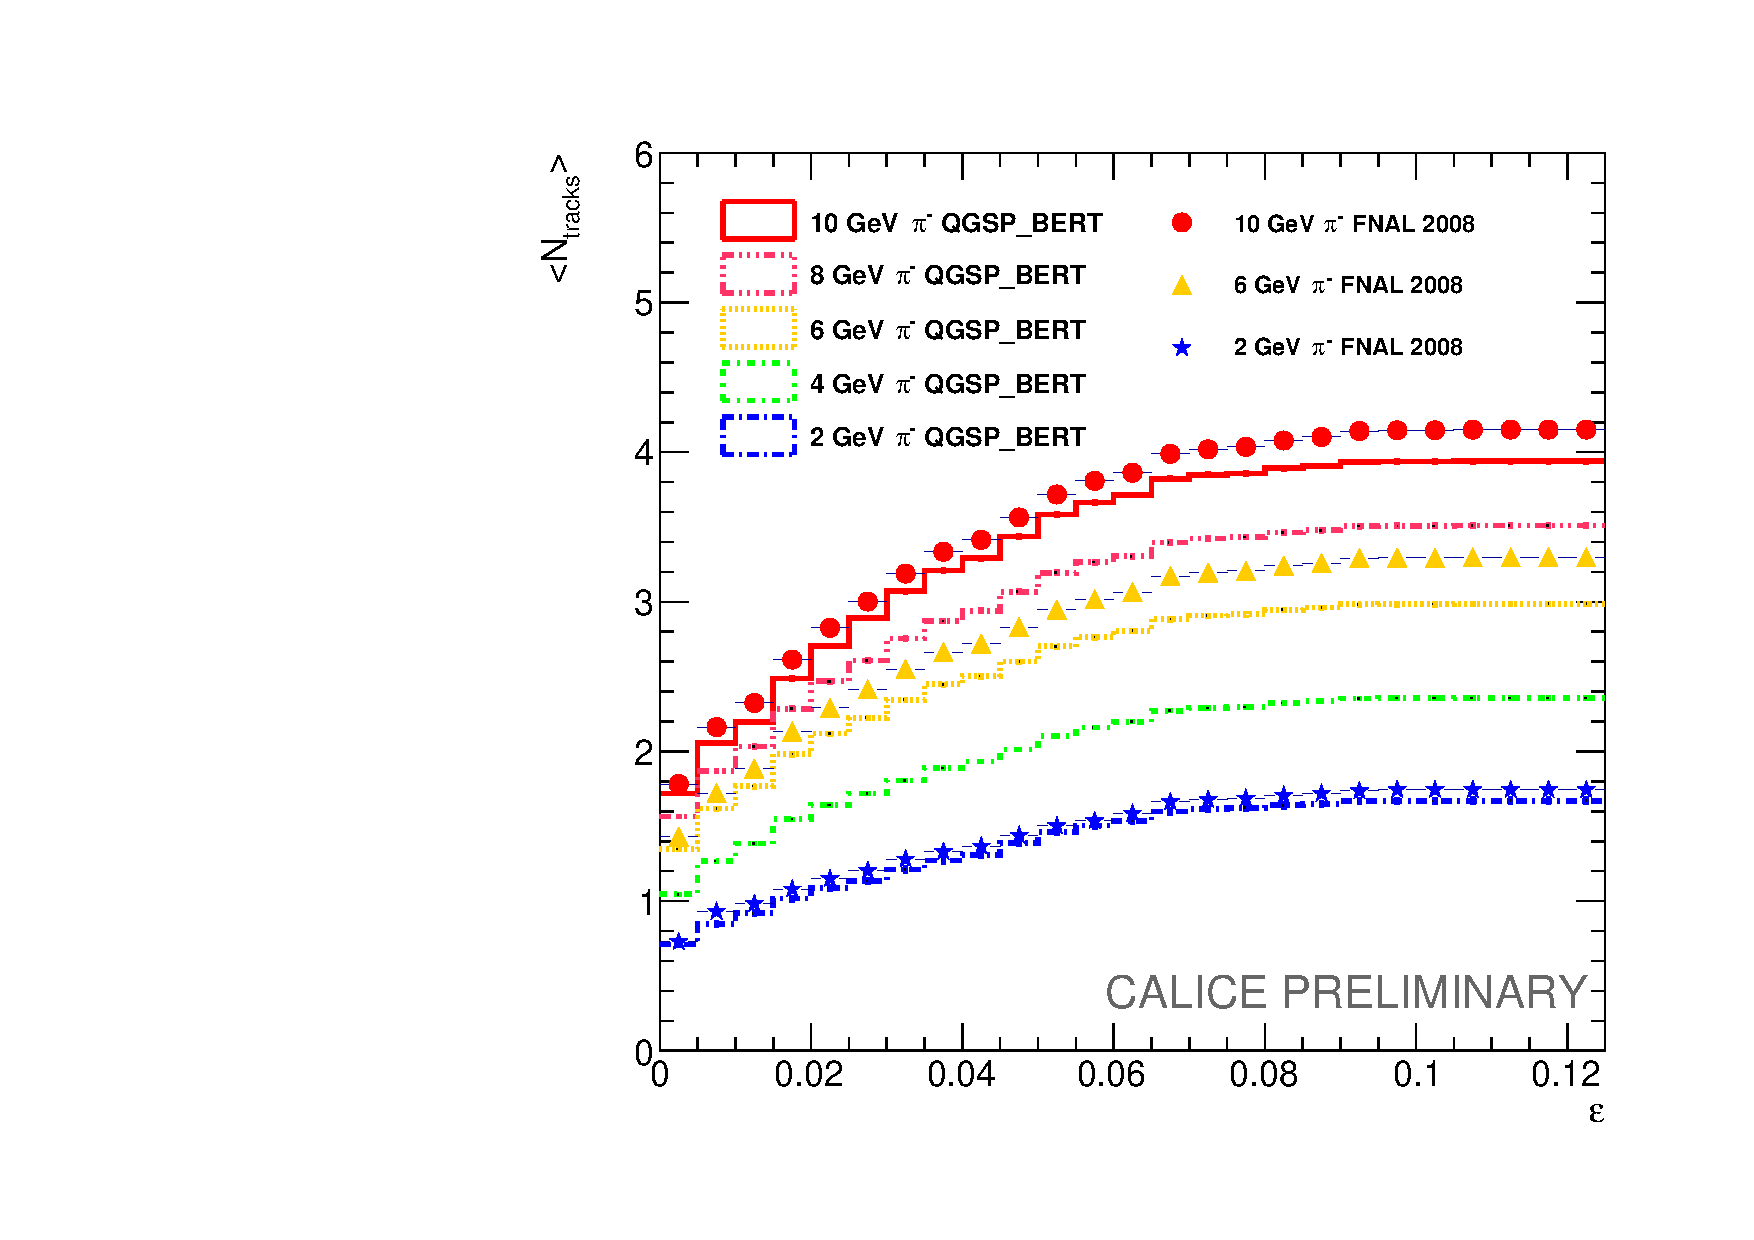
\includegraphics[width=0.5\textwidth]{ECAL/plots/combination.pdf}
		\caption{\label{fig:epsilonsysdata} \sl Mean number of tracks found by the \tfa\ as a function of $\varepsilon$ values for 2, 4, 6, 8 and 10\,GeV beam energy for data (bullets) and for \qgsp\ physics list simulation (lines). Events without a detected interaction region are excluded.}
	\end{figure}
	
	For future reference the Fig. \ref{fig:epsilonsysdata} shows a comparison between data and Monte Carlo for the studies presented in Sec.~\ref{sec:systematics}. 
	
	\section{Polar angle and track length as a function of the \ep}\label{app:b}
	
	Figure \ref{fig:thetaepsilonsys} presents the variation of $\left<\theta\right>$ in \qgsp\ simulation  for different beam energies as a function of the \ep\ value. 
	The mean polar angle saturates for large $\varepsilon$. The empirically chosen value of $\varepsilon=0.03$ is close to a local minimum of the function, therefore, the $<\theta>$ observable is stable against a small variation of the $\varepsilon$ value. 
	
	The mean track length $<l>$ as function of $\varepsilon$ for different beam energies is shown in Fig. \ref{fig:lepsilonsys}. 
	The function has a local maximum around $\varepsilon=0.03$ and it saturates for large $\varepsilon$. 
	These observations can be explained as follows:
	\begin{itemize}
		\item At $\varepsilon \to 0$ only small pencil-like clusters are considered as tracks. The small tracks can fit the \ecal\ pad volume for any direction. Therefore, $<\theta>$ is large; 
		\item If the $\varepsilon$ value is slightly above zero, the longer clusters, with some amount of adjacent hits become tracks. These tracks have smaller $<\theta>$ angle due to a fact that the \ecalp\ has 30 layers in depth and 18 $\times$ 18 lateral size.  
		\item With large $\varepsilon$ values also spherical shaped clusters are accepted as tracks. These clusters have a small amount of hits, since otherwise, they would be counted as an interaction region. The algorithm can assign any direction for these spherical clusters, resulting in an increase of $\left<\theta\right>$ and a decrease of the mean track length. 
	\end{itemize}
	
	
	
	\begin{figure}[H]
		\centering
		\begin{subfigure}{0.5\textwidth}
			\centering
			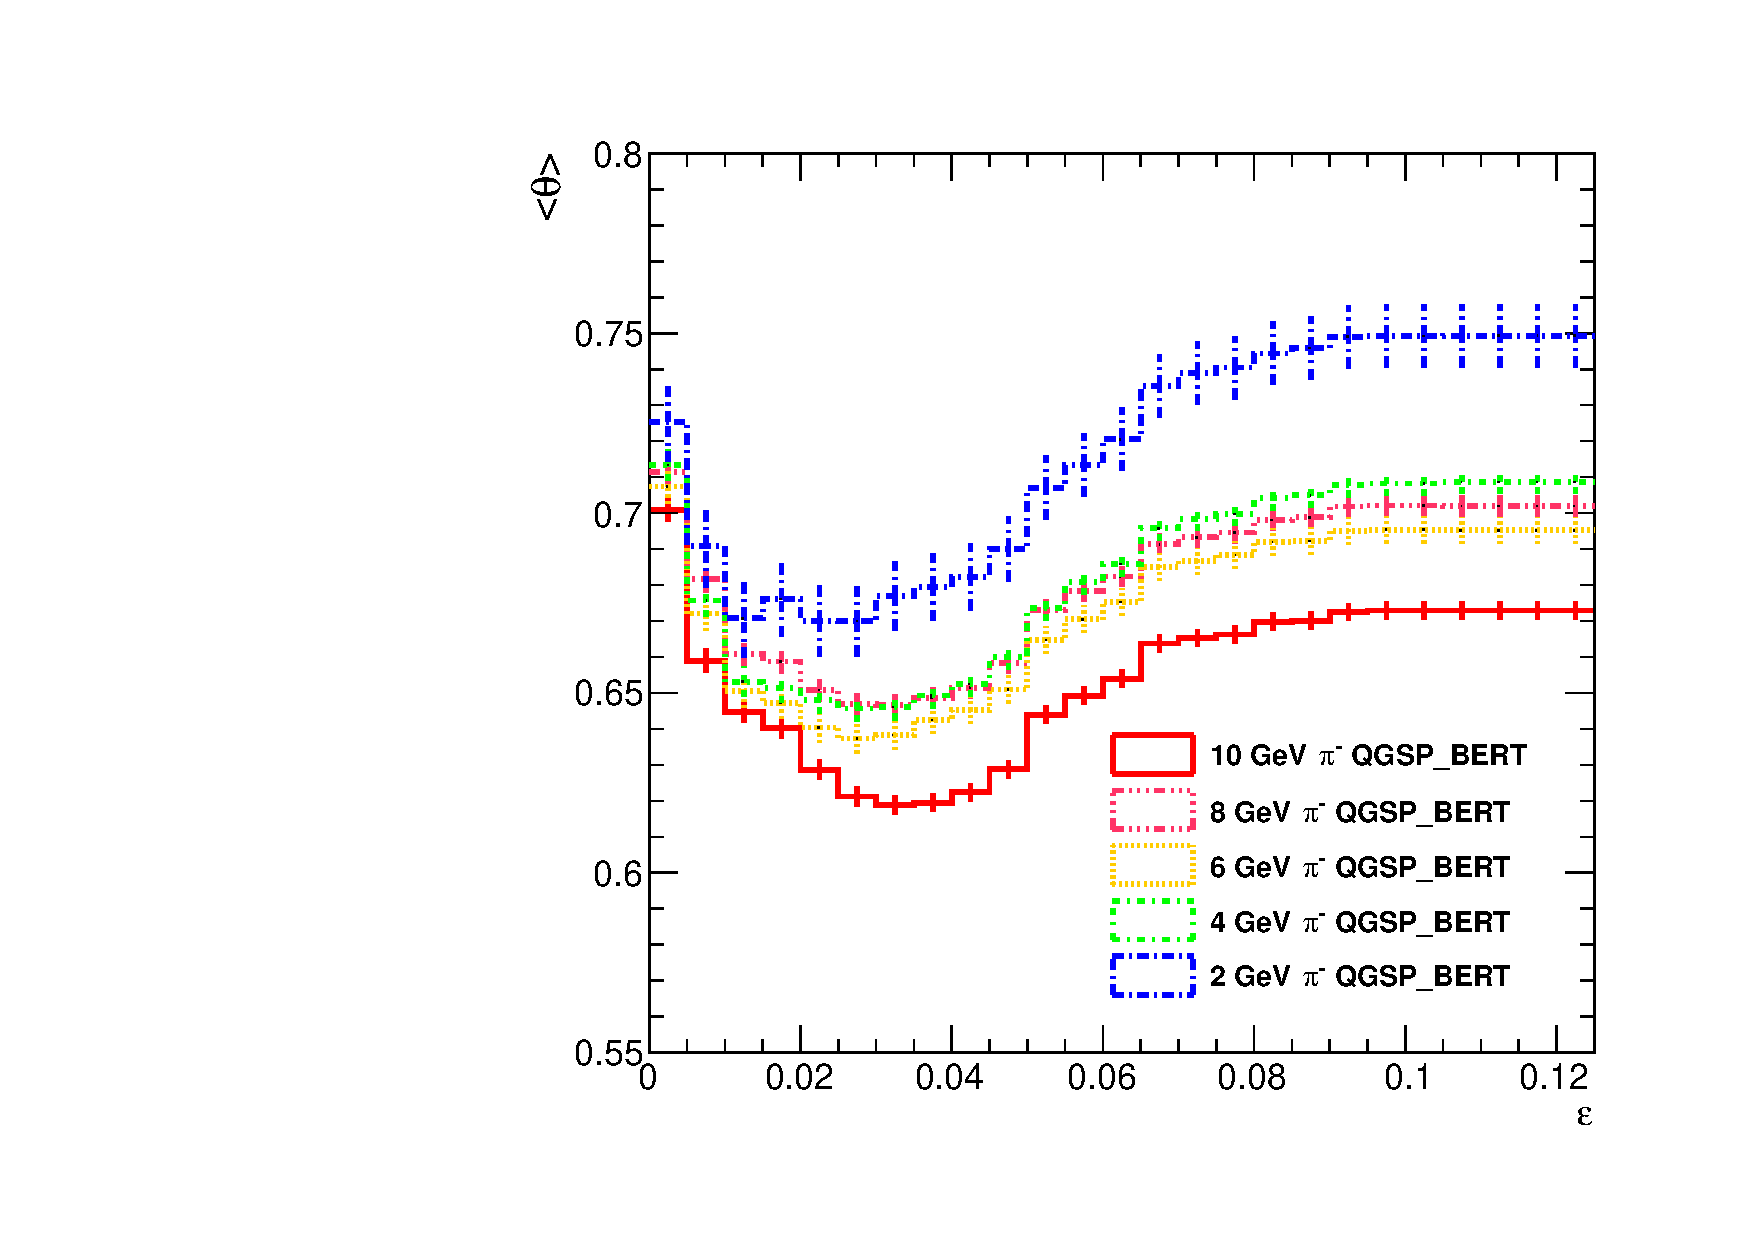
\includegraphics[width=.90\linewidth]{ECAL/plots/sys-theta.pdf}
			\caption{\label{fig:thetaepsilonsys} }
		\end{subfigure}% 
		\begin{subfigure}{0.5\textwidth}
			\centering
			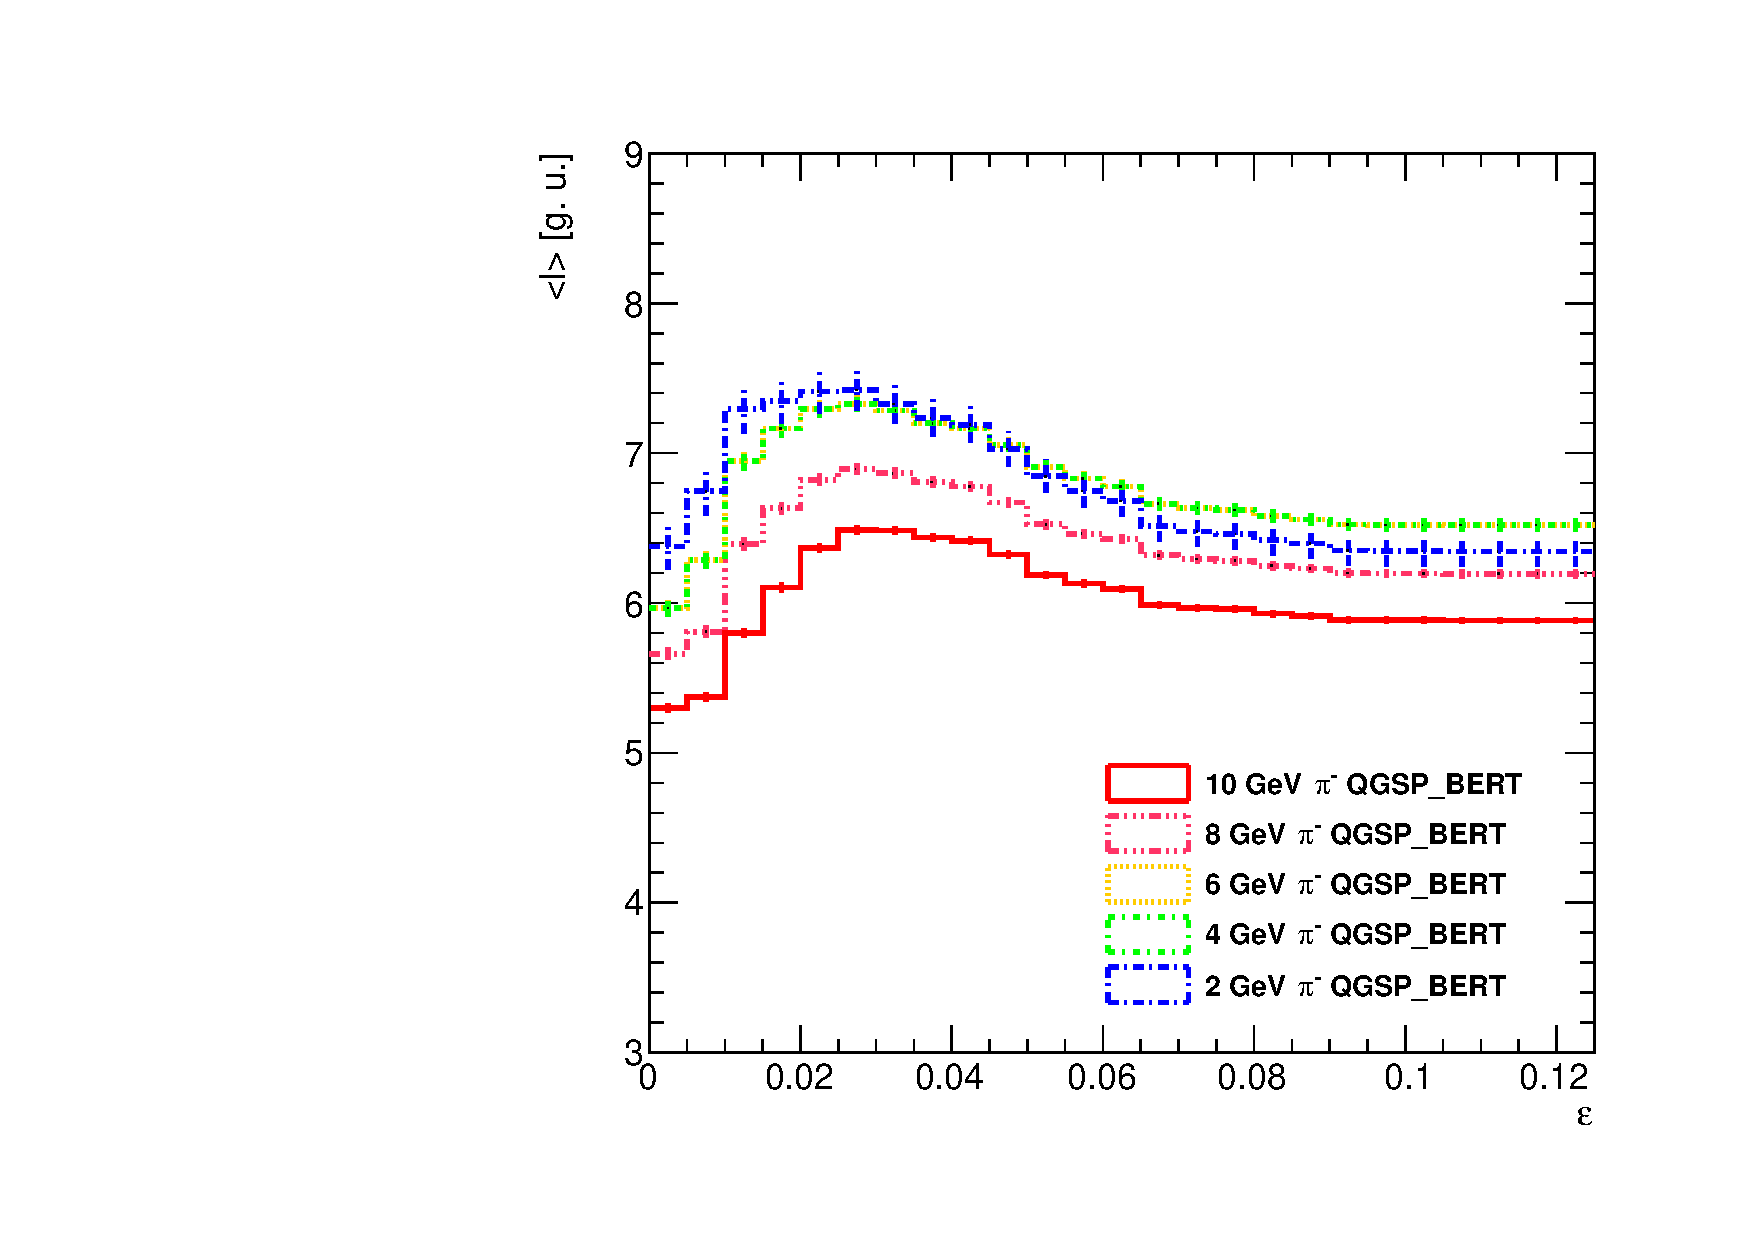
\includegraphics[width=.90\linewidth]{ECAL/plots/sys-l.pdf}
			\caption{\label{fig:lepsilonsys} }
		\end{subfigure}
		\caption{\label{fig:syslthetaexample} \sl Mean $\theta$ angle (a) and mean track length $l$ (b) of the tracks found by the \tfa\ with different \ep\ values for 2, 4, 6, 8 and 10\,GeV beam energy in \qgsp\ simulation. The minimum value of $\left<\theta\right>$ and the maximum value of the track length is around the empirically chosen value of $0.03$. }
	\end{figure}
	
\end{appendices}
%The following plots in Fig. \ref{fig:rtotexample} and \ref{fig:rtotalrgraph} allow to establish a connection between Ref. \cite{bib:Naomi} and the present study. Regarding the difference in units of measurement and different selection by interaction layer, the Fig. \ref{fig:rtotalrgraph} is similar to its analogue in Ref. \cite{bib:Naomi}.
%\begin{figure}[H]
%\centering
%\begin{subfigure}{0.5\textwidth}
%\centering
%\includegraphics[width=.90\linewidth]{ECAL/plots/r-total-2.pdf}
%\caption{\label{fig:rtot2} 2\,GeV primary particle.}
%\end{subfigure}% 
%\begin{subfigure}{0.5\textwidth}
%\centering
%\includegraphics[width=.90\linewidth]{ECAL/plots/r-total-10.pdf}
%\caption{\label{fig:rtot10} 10\,GeV primary particle.}
%\end{subfigure}
%\caption{\label{fig:rtotexample} A comparison of mean radius of event hits between Monte Carlo samples and data with 2 (left) and 10 (right) GeV beam energy. The histograms are normalized to unity in order to compare samples with different event number. Error bars on the plot represent statistical uncertainties only.}
%\end{figure}

%\begin{figure}[H]
%\centering
%\includegraphics[width=0.5\textwidth]{ECAL/plots/r-total-graph.pdf}
%\caption{\label{fig:rtotalrgraph} A mean radius of hits in the \ecal\ for data and various Monte Carlo physics lists as a function of beam energy (2\,GeV to 10\,GeV). Error regions on the graph represent statistical uncertainties only.}
%\end{figure}

%\begin{figure}[H]
%\centering
%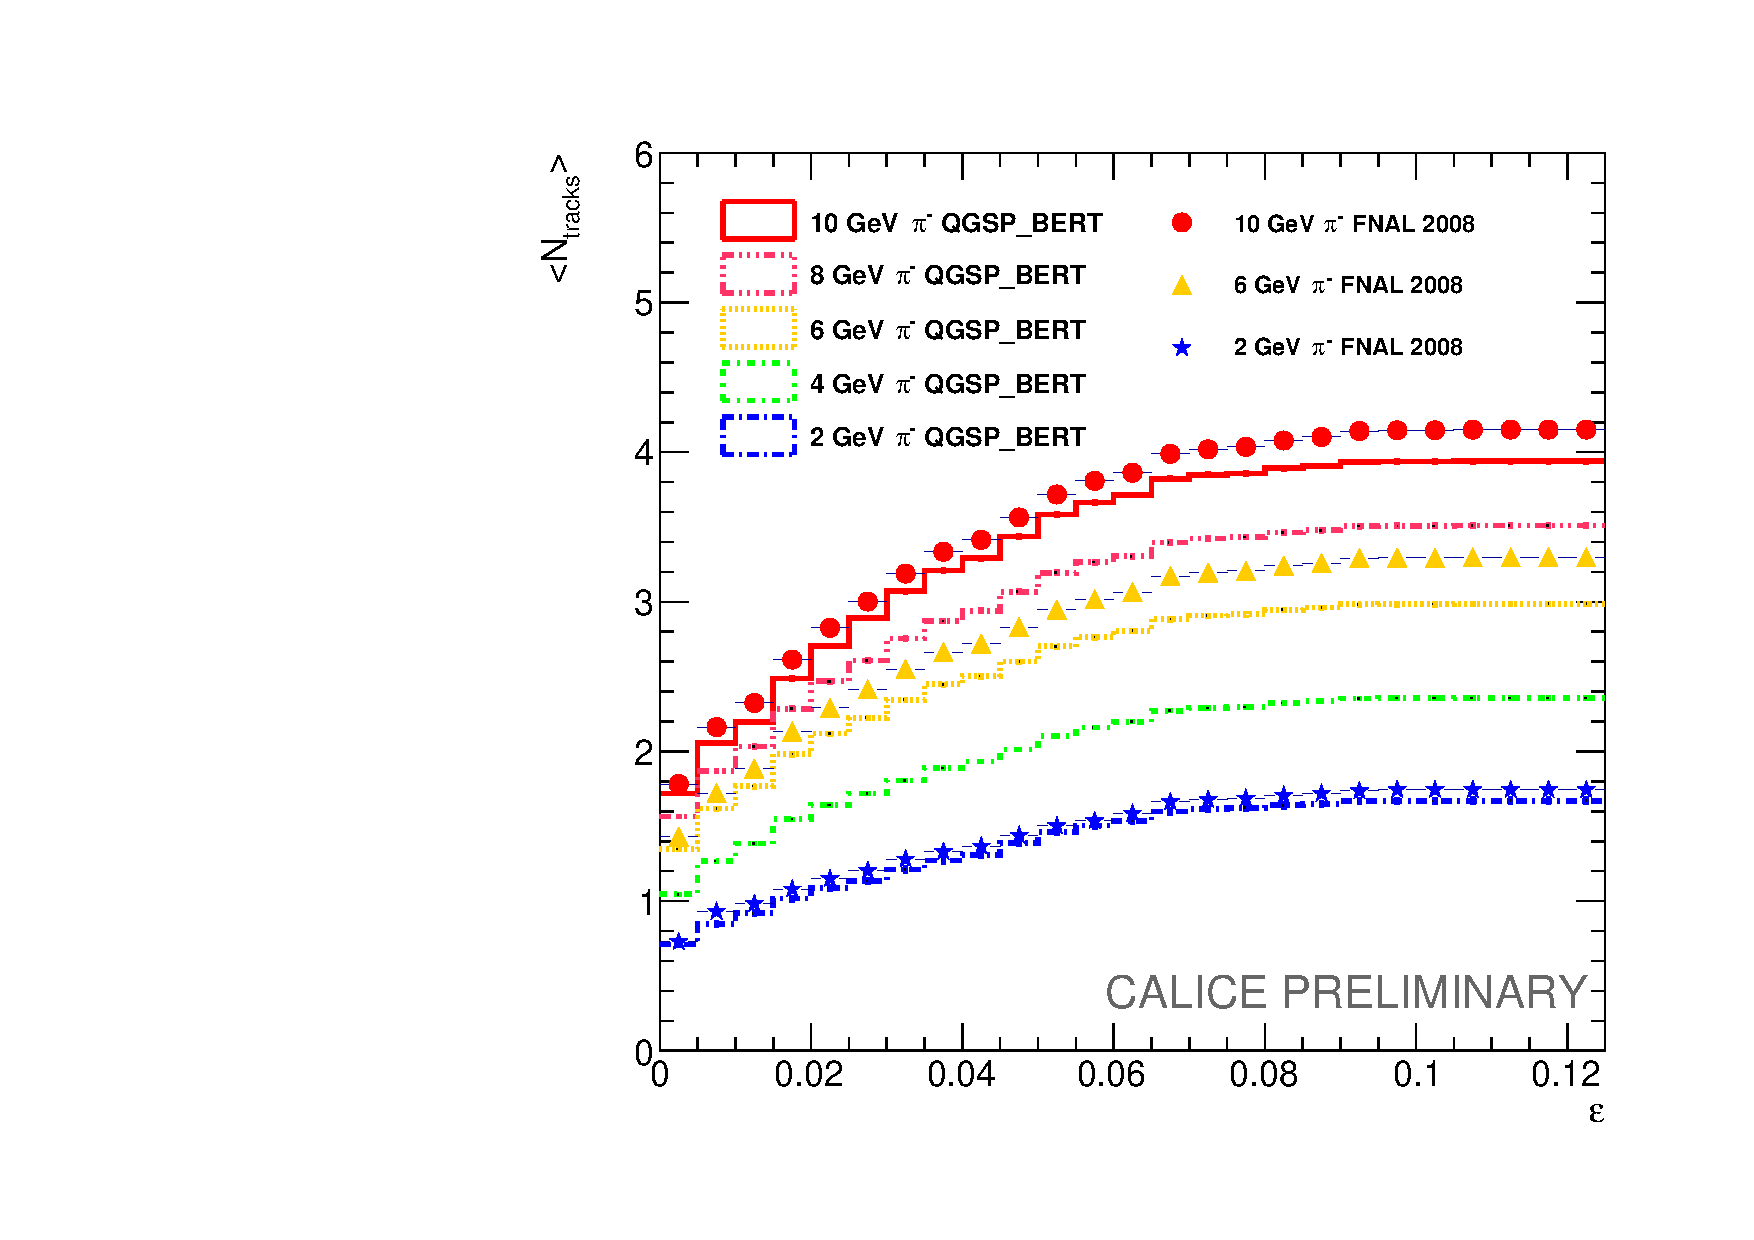
\includegraphics[width=0.5\textwidth]{ECAL/plots/combination.pdf}
%\caption{\label{fig:epsilondatasys} Mean number of tracks found by the \tfa\ with different \ep\ values for 2, 4, 6, 8 and 10\,GeV beam energy of the \qgsp\ simulation and data. The difference between data and corresponding simulation curves is caused by an underestimation of number of clusters by the physics list model. The saturation value of $<N_{tracks}>$ is gradually increasing with the beam energy. }
%\end{figure}

